% ==========================================================================
%  PFC 2026 (VF) - Versao Final, revisada apos a apresentacao
%  Planejamento de Trajetoria para Robo Terrestre Usando Grafos
%  Autores: Gabriel Dias Vilela e Tassandro Cavalcante Leitao
%  Instituto Militar de Engenharia
% ==========================================================================
\documentclass[
    12pt,
    openright,
    oneside,
    a4paper,
    english,
    brazil
]{abntex2}

% -- Pacotes --------------------------------------------------------------
\usepackage[utf8]{inputenc}
\usepackage[T1]{fontenc}
\usepackage{lmodern}
\usepackage{indentfirst}
\usepackage{graphicx}
\usepackage{microtype}
\usepackage{amsmath,amssymb}
\usepackage{booktabs}
\usepackage{multirow}
\usepackage{array}
\usepackage{hyperref}
\usepackage{float}
\usepackage{listings}
\usepackage{xcolor}
\usepackage{colortbl}
\usepackage{tikz}
\usetikzlibrary{positioning, arrows.meta, shapes.geometric, fit, backgrounds, calc}
\usepackage[brazilian,hyperpageref]{backref}
\usepackage[alf]{abntex2cite}

% -- Estilos TikZ globais para os diagramas do projeto ---------------------
\definecolor{boxBlue}{HTML}{2E86AB}
\definecolor{boxGreen}{HTML}{56B870}
\definecolor{boxOrange}{HTML}{E07B39}
\definecolor{boxPurple}{HTML}{8E5BB5}
\definecolor{boxGray}{HTML}{6C757D}
\definecolor{rosNavy}{HTML}{14284B}

\tikzset{
    pipelineBox/.style={
        rectangle, rounded corners=4pt, draw=#1, fill=#1!12, line width=0.9pt,
        minimum width=2.8cm, minimum height=1.5cm, align=center,
        inner sep=4pt, font=\small\sffamily, text=black
    },
    pipelineArrow/.style={
        -{Stealth[length=3mm, width=2mm]}, line width=0.9pt, draw=boxGray
    },
    compBox/.style={
        rectangle, rounded corners=3pt, draw=#1, fill=#1!10, line width=0.7pt,
        minimum width=5.6cm, minimum height=0.9cm, align=center,
        font=\footnotesize\sffamily, text=black
    },
    compTitle/.style={
        rectangle, rounded corners=3pt, fill=#1, line width=0.7pt,
        minimum width=5.6cm, minimum height=0.95cm, align=center,
        font=\small\bfseries\sffamily, text=white
    },
    compArrow/.style={
        -{Stealth[length=2.5mm, width=1.8mm]}, line width=0.7pt, draw=#1
    }
}

% -- Configuracao de listings ---------------------------------------------
\lstset{
    language=Python,
    basicstyle=\ttfamily\small,
    keywordstyle=\color{blue}\bfseries,
    stringstyle=\color{red},
    commentstyle=\color{gray}\itshape,
    numbers=left,
    numberstyle=\tiny\color{gray},
    breaklines=true,
    frame=single,
    captionpos=b,
}

% Estilo para comandos de terminal (Apendice A)
\lstdefinestyle{comandos}{
    language=bash,
    basicstyle=\ttfamily\footnotesize,
    keywordstyle=\color{black},
    stringstyle=\color{black},
    commentstyle=\color{gray}\itshape,
    numbers=none,
    breaklines=true,
    frame=single,
    backgroundcolor=\color{gray!6},
    rulecolor=\color{gray!50},
    columns=fullflexible,
    keepspaces=true,
    showstringspaces=false,
    xleftmargin=2pt,
    xrightmargin=2pt,
}

% -- Dados do documento ---------------------------------------------------
\titulo{Planejamento de Trajetória para Robô Terrestre Usando Grafos}
\autor{Gabriel Dias Vilela \and Tassandro Cavalcante Leitão}
\local{Rio de Janeiro}
\data{2026}
\orientador{Claudia Marcela Justel, D.Sc.}
\coorientador{Paulo Fernando Ferreira Rosa, Ph.D.}
\instituicao{%
    MINISTÉRIO DA DEFESA\\
    EXÉRCITO BRASILEIRO\\
    DEPARTAMENTO DE CIÊNCIA E TECNOLOGIA\\
    INSTITUTO MILITAR DE ENGENHARIA\\
    CURSO DE GRADUAÇÃO EM ENGENHARIA DA COMPUTAÇÃO
}
\tipotrabalho{Projeto de Final de Curso}
\preambulo{Projeto de Final de Curso apresentado ao Curso de Graduação em Engenharia da Computação do Instituto Militar de Engenharia, como requisito parcial para a obtenção do título de Bacharel em Engenharia da Computação.}

% ==========================================================================
\begin{document}

\selectlanguage{brazil}
\frenchspacing

% ==========================================================================
%  ELEMENTOS PRE-TEXTUAIS
% ==========================================================================
\pretextual

% -- Capa -----------------------------------------------------------------
\begin{capa}
    \center
    \ABNTEXchapterfont

    {\normalsize
    MINISTÉRIO DA DEFESA\\
    EXÉRCITO BRASILEIRO\\
    DEPARTAMENTO DE CIÊNCIA E TECNOLOGIA\\
    INSTITUTO MILITAR DE ENGENHARIA\\
    CURSO DE GRADUAÇÃO EM ENGENHARIA DA COMPUTAÇÃO}

    \vspace*{2cm}

    {\large GABRIEL DIAS VILELA}\\
    {\large TASSANDRO CAVALCANTE LEITÃO}

    \vspace*{3cm}

    {\Large\bfseries PLANEJAMENTO DE TRAJETÓRIA PARA ROBÔ TERRESTRE USANDO GRAFOS}

    \vfill

    {\large RIO DE JANEIRO}\\
    {\large 2026}
\end{capa}

% -- Folha de rosto -------------------------------------------------------
\begin{folhaderosto}
    \center
    {\large GABRIEL DIAS VILELA}\\
    {\large TASSANDRO CAVALCANTE LEITÃO}

    \vspace*{3cm}

    {\Large\bfseries PLANEJAMENTO DE TRAJETÓRIA PARA ROBÔ TERRESTRE USANDO GRAFOS}

    \vspace*{2cm}

    \hspace{.45\textwidth}
    \begin{minipage}{.5\textwidth}
        \imprimirpreambulo\\[1em]
        Orientador(es): Claudia Marcela Justel, D.Sc.\\
        Paulo Fernando Ferreira Rosa, Ph.D.
    \end{minipage}

    \vfill

    {\large Rio de Janeiro}\\
    {\large 2026}
\end{folhaderosto}

% -- Ficha catalografica --------------------------------------------------
\begin{fichacatalografica}
    \vspace*{\fill}
    \begin{center}
    {\normalsize \copyright 2026\\
    INSTITUTO MILITAR DE ENGENHARIA\\
    Praça General Tibúrcio, 80 -- Praia Vermelha\\
    Rio de Janeiro -- RJ CEP: 22290-270}
    \end{center}

    \vspace{1cm}

    \noindent Este exemplar é de propriedade do Instituto Militar de Engenharia, que poderá incluí-lo em base de dados, armazenar em computador, microfilmar ou adotar qualquer forma de arquivamento.

    É permitida a menção, reprodução parcial ou integral e a transmissão entre bibliotecas deste trabalho, sem modificação de seu texto, em qualquer meio que esteja ou venha a ser fixado, para pesquisa acadêmica, comentários e citações, desde que sem finalidade comercial e que seja feita a referência bibliográfica completa.

    Os conceitos expressos neste trabalho são de responsabilidade do(s) autor(es) e do(s) orientador(es).

    \vspace{1cm}

    \noindent
    Dias Vilela, Gabriel; Cavalcante Leitão, Tassandro.\\
    Planejamento de trajetória para robô terrestre usando grafos / Gabriel Dias Vilela e Tassandro Cavalcante Leitão. -- Rio de Janeiro, 2026.\\
    78 f.\\[0.5em]
    Orientador(es): Claudia Marcela Justel e Paulo Fernando Ferreira Rosa.\\[0.5em]
    Projeto de Final de Curso (graduação) -- Instituto Militar de Engenharia, Engenharia da Computação, 2026.\\[0.5em]
    1.~Veículos terrestres não tripulados. 2.~Segmentação semântica. 3.~Algoritmos baseados em grafos. 4.~Planejamento de trajetórias. 5.~Robot Operating System. i.~Justel, Claudia Marcela (orient.) ii.~Ferreira Rosa, Paulo Fernando (orient.) iii.~Título
    \vspace*{\fill}
\end{fichacatalografica}

% -- Folha de aprovacao ---------------------------------------------------
\begin{folhadeaprovacao}
    \center

    {\large GABRIEL DIAS VILELA}\\
    {\large TASSANDRO CAVALCANTE LEITÃO}

    \vspace{1cm}

    {\large\bfseries Planejamento de trajetória para robô terrestre usando grafos}

    \vspace{1cm}

    Projeto de Final de Curso apresentado ao Curso de Graduação em Engenharia da Computação do Instituto Militar de Engenharia, como requisito parcial para a obtenção do título de Bacharel em Engenharia da Computação.

    \vspace{0.5cm}

    Orientador(es): Claudia Marcela Justel e Paulo Fernando Ferreira Rosa.

    \vspace{0.5cm}

    Aprovada em \_\_\_ de \_\_\_\_\_\_\_\_\_\_\_ de 2026, pela seguinte banca examinadora:

    \vspace{1.5cm}

    \assinatura{Prof. Paulo Fernando Ferreira Rosa -- Professor do IME}
    \assinatura{Profa. Claudia Marcela Justel -- Professora do IME}
    \assinatura{Maj Diogo Pimentel Pinheiro -- Centro Tecnológico do Exército}
    \assinatura{Cel Anderson Fernandes Pereira dos Santos -- Coordenador do PFC -- IME}

    \vfill

    {\large Rio de Janeiro}\\
    {\large 2026}
\end{folhadeaprovacao}

% -- Dedicatoria ----------------------------------------------------------
\begin{dedicatoria}
    \vspace*{\fill}
    \centering
    \noindent
    \textit{Às nossas famílias.}
    \vspace*{\fill}
\end{dedicatoria}

% -- Agradecimentos -------------------------------------------------------
\begin{agradecimentos}
Os agradecimentos principais são direcionados aos nossos orientadores por todo acompanhamento e ensinamentos. Agradecemos também ao Major Fábio Luiz Junior, cujos modelos de segmentação e trabalho de referência sobre planejamento em mapas de navegabilidade fundamentam este projeto, e aos autores do projeto anterior, João Vitor Camelo de Almeida e Thiago Calheiros de Souza Barbosa, cujo trabalho serviu de base e inspiração para o presente projeto.
\end{agradecimentos}

% -- Epigrafe -------------------------------------------------------------
\begin{epigrafe}
    \vspace*{\fill}
    \begin{flushright}
        \textit{``Não vos amoldeis às estruturas deste mundo,\\
        mas transformai-vos pela renovação da mente,\\
        a fim de distinguir qual é a vontade de Deus:\\
        o que é bom, o que Lhe é agradável, o que é perfeito.''}\\
        (Bíblia Sagrada, Romanos 12, 2)
    \end{flushright}
\end{epigrafe}

% -- Resumo ---------------------------------------------------------------
\setlength{\absparsep}{18pt}
\begin{resumo}
Este trabalho trata do planejamento de trajetória para veículos terrestres não tripulados (UGV) a partir de imagens aéreas obtidas por veículos aéreos não tripulados (UAV), em continuidade ao Projeto de Final de Curso de mesmo tema desenvolvido em 2025. Foi projetada e implementada uma arquitetura de \textit{software} modular e orientada a objetos, organizada em cinco estágios encadeados: ingestão de dados, pré-processamento, construção de grafos, algoritmos e pós-processamento. As áreas transitáveis são identificadas por segmentação semântica, técnica de aprendizado de máquina na qual uma rede neural do tipo U-Net, pré-treinada sobre o \textit{Semantic Drone Dataset} \cite{drone_dataset} e disponibilizada em \cite{junior2024_models}, classifica cada pixel da imagem. O mapa de navegabilidade resultante é convertido em um grafo, sobre o qual são comparados os algoritmos de busca BFS, DFS, Dijkstra e A* e o planejador por amostragem \textit{Rapidly-exploring Random Tree} (RRT). O caminho calculado é enviado ao robô por meio do \textit{Robot Operating System} (ROS 2) \cite{quigley2009} e percorrido por um UGV simulado (Clearpath Jackal) no simulador Gazebo \cite{koenig2004}. Foi desenvolvida ainda a geração automática de mapas de ocupação a partir da descrição do mundo simulado, de modo que o caminho planejado e o mundo do simulador compartilhem o mesmo referencial métrico. Os ensaios em ambiente virtual foram concluídos com êxito: o robô simulado percorre integralmente as trajetórias planejadas, tanto sobre o mapa de ocupação do próprio mundo simulado quanto sobre uma imagem aérea real obtida por UAV no Outeiro da Glória, no Rio de Janeiro. A validação em ambiente real, prevista no planejamento inicial do projeto, não pôde ser realizada dentro do prazo do projeto por restrições de acesso a plataforma física, de espaço de ensaio e de tempo, e permanece como a etapa imediata de continuidade.

\textbf{Palavras-chave}: Veículos terrestres não tripulados; Segmentação semântica; Aprendizado de máquina; Algoritmos baseados em grafos; Planejamento de trajetórias; RRT; ROS; Simulador Gazebo.
\end{resumo}

% -- Abstract -------------------------------------------------------------
\begin{resumo}[Abstract]
\begin{otherlanguage*}{english}
This work addresses trajectory planning for unmanned ground vehicles (UGV) from aerial images acquired by unmanned aerial vehicles (UAV), as a continuation of the undergraduate final project on the same subject developed in 2025. A modular, object-oriented software architecture was designed and implemented, organized into five chained stages: data ingestion, preprocessing, graph construction, algorithms, and post-processing. Traversable areas are identified by semantic segmentation, a machine learning technique in which a U-Net neural network, pre-trained on the Semantic Drone Dataset \cite{drone_dataset} and released in \cite{junior2024_models}, classifies every pixel of the image. The resulting navigability map is converted into a graph, on which the BFS, DFS, Dijkstra, and A* search algorithms and the sampling-based Rapidly-exploring Random Tree (RRT) planner are compared. The computed path is published on the Robot Operating System (ROS 2) \cite{quigley2009} and driven by a simulated UGV (Clearpath Jackal) in the Gazebo simulator \cite{koenig2004}. The automatic generation of occupancy maps from the description of the simulated world was also developed, so that the planned path and the simulator world share the same metric frame. The virtual environment trials were completed successfully: the simulated robot drives the full planned trajectories, both over the occupancy map of the simulated world itself and over a real aerial image acquired by a UAV at Outeiro da Glória, in Rio de Janeiro. Validation in a real environment, foreseen in the initial project plan, could not be carried out within the project deadline due to restrictions on access to a physical platform, on test area, and on time, and remains the immediate continuation step.

\textbf{Keywords}: Unmanned ground vehicles; Semantic segmentation; Machine learning; Graph-based algorithms; Trajectory planning; RRT; ROS; Gazebo simulator.
\end{otherlanguage*}
\end{resumo}

% -- Listas ---------------------------------------------------------------
\pdfbookmark[0]{\listfigurename}{lof}
\listoffigures*
\cleardoublepage

\pdfbookmark[0]{\listtablename}{lot}
\listoftables*
\cleardoublepage

% -- Lista de abreviaturas e siglas ---------------------------------------
\begin{siglas}
    \item[BFS] Breadth-First Search
    \item[CNN] Convolutional Neural Network
    \item[CTEx] Centro Tecnológico do Exército
    \item[DDS] Data Distribution Service
    \item[DFS] Depth-First Search
    \item[EB] Exército Brasileiro
    \item[EKF] Extended Kalman Filter
    \item[GSD] Ground Sampling Distance
    \item[IA] Inteligência Artificial
    \item[IMU] Inertial Measurement Unit
    \item[LiDAR] Light Detection and Ranging
    \item[mIoU] Mean Intersection over Union
    \item[OOP] Object-Oriented Programming
    \item[PFC] Projeto de Final de Curso
    \item[QoS] Quality of Service
    \item[ROS] Robot Operating System
    \item[RRT] Rapidly-exploring Random Tree
    \item[SDD] Semantic Drone Dataset
    \item[SDF] Simulation Description Format
    \item[SVTRP] Sistemas de Veículos Terrestres Remotamente Pilotados
    \item[UAV] Unmanned Aerial Vehicle
    \item[UGV] Unmanned Ground Vehicle
    \item[WSL] Windows Subsystem for Linux
\end{siglas}

% -- Sumario --------------------------------------------------------------
\pdfbookmark[0]{\contentsname}{toc}
\tableofcontents*
\cleardoublepage

% ==========================================================================
%  ELEMENTOS TEXTUAIS
% ==========================================================================
\textual

% ======================================================================
\chapter{INTRODUÇÃO}
% ======================================================================

Os avanços tecnológicos envolvendo visão computacional, eletrônica e inteligência artificial, entre outras áreas correlatas, impulsionaram a tendência de desenvolvimento e uso de ferramentas que automatizam as disputas em ambientes de combate. Nesse sentido, com a possibilidade de aumentar a eficácia operacional e reduzir a participação e desgaste humano (física, cognitiva e psicologicamente) no campo de batalha, a integração de robôs autônomos nesses cenários de confronto é iminente e torna-se motivo de vantagem tática e estratégica. O mesmo raciocínio se aplica a tarefas de resgate em eventos extremos, como terremotos, chuvas intensas e acidentes com material radioativo, nas quais o emprego de robôs autônomos permite atuar em áreas perigosas reduzindo a exposição de pessoas.

Em relação à autonomia desses sistemas, o planejamento de trajetória de robôs terrestres é uma das tarefas essenciais a ser realizada e ela se encontra dentro de um escopo multidisciplinar que inclui conhecimentos em diversas áreas de grande complexidade, como a robótica e a teoria dos grafos. Essas disciplinas convergem na modelagem do cenário de combate como um grafo, no qual os vértices representam as posições transitáveis pelos robôs no mapa e as arestas definem os caminhos. Dessa maneira, algoritmos de busca e otimização são ferramentas que guiam o planejamento das possíveis rotas, auxiliando na coordenação entre pontos e adaptação aos obstáculos.

A pesquisa ``Cooperação Entre Plataformas Terrestres e Aéreas para Aquisição, Rastreamento e Perseguição de Alvos, Utilizando Visão Computacional e Inteligência Artificial'' \cite{junior2024}, que se encontra em fase de desenvolvimento no laboratório LIARC, iniciada em 2023 pelo Major Fábio Luiz Junior, aborda o emprego de plataformas robóticas aéreas (UAV) e terrestres (UGV) em ambientes de batalha e como essas duas estruturas podem trabalhar em conjunto para otimizar e ampliar o poder de ataque e estratégico militar.

% -- 1.1 -------------------------------------------------------------------
\section{Contribuições do PFC 2025}
\label{sec:pfc2025}

O presente projeto é uma continuação direta do trabalho ``Planejamento de Trajetória para Robô Terrestre, Utilizando Otimização em Grafos'', Projeto de Final de Curso defendido em 2025 por João Vitor Camelo de Almeida e Thiago Calheiros de Souza Barbosa \cite{camelo2025}, doravante chamado de PFC 2025. Naquele trabalho, os autores propuseram uma abordagem baseada em grafos para o planejamento de caminhos sobre imagens aéreas já segmentadas, implementando os algoritmos de Dijkstra e A* e comparando-os com o algoritmo estocástico RRT.

As principais conclusões do PFC 2025 foram:

\begin{itemize}
    \item Os algoritmos baseados em grafos (Dijkstra e A*) apresentaram desempenho mais consistente, confiável e previsível em relação ao RRT, destacando-se pelo determinismo e pela garantia de otimalidade das soluções;
    \item O algoritmo A* mostrou-se ligeiramente mais rápido que o Dijkstra, explorando um menor número de vértices, sendo considerado mais adequado ao problema proposto;
    \item A inserção de pesos nas arestas do grafo, com base na proximidade a obstáculos, produziu caminhos mais realistas que se distanciam de regiões de risco, sem impacto significativo no tempo de execução;
    \item O RRT apresentou dificuldades em imagens com áreas transitáveis estreitas, excedendo o tempo limite em dois dos cinco cenários testados;
    \item A abordagem proposta, ao integrar segmentação semântica de imagens e planejamento baseado em grafos, constitui uma alternativa promissora para aplicações em veículos autônomos.
\end{itemize}

O PFC 2025 apontou três frentes de continuidade: o tratamento de ambientes dinâmicos, a avaliação do uso de grafos em composição de imagens em tempo real e a extensão da segmentação semântica para uma variedade maior de terrenos. Este projeto concentrou-se na terceira frente e acrescentou uma quarta, não prevista naquele trabalho: a execução efetiva do caminho planejado por um veículo, ainda que simulado.

% -- 1.2 -------------------------------------------------------------------
\section{Etapas do Projeto}
\label{sec:evolucao}

O desenvolvimento deste projeto foi organizado em três etapas sucessivas, cada uma construída sobre a anterior.

Na \textbf{primeira etapa}, de planejamento e estruturação, foram definidos o escopo do trabalho e a arquitetura de \textit{software}, modular e orientada a objetos, com cinco módulos encadeados, interfaces abstratas e padrões de fábrica. Foram também implementados os algoritmos de busca em grafos BFS, DFS, Dijkstra e A*, tomando como entrada um mapa de navegabilidade com cores fixas.

Na \textbf{segunda etapa}, a arquitetura recebeu três acréscimos, que a completaram desde a imagem aérea até o veículo:

\begin{enumerate}
    \item \textbf{Inclusão do algoritmo RRT.} O planejador baseado em amostragem \textit{Rapidly-exploring Random Tree} \cite{lavalle1998} foi adicionado ao módulo de algoritmos, junto aos algoritmos de busca em grafos BFS, DFS, Dijkstra e A*, sob a mesma interface. Isso permite contrastar diretamente, sobre os mesmos mapas, o comportamento de um planejador estocástico com o dos algoritmos determinísticos, dando continuidade à comparação feita no PFC 2025.

    \item \textbf{Implementação da segmentação semântica.} A identificação das áreas transitáveis, antes dependente de mapas previamente segmentados, passou a ser realizada dentro do próprio \textit{pipeline} por meio dos modelos de redes neurais U-Net pré-treinados disponibilizados em \cite{junior2024_models}, treinados sobre o \emph{Semantic Drone Dataset} \cite{drone_dataset}. O módulo de pré-processamento executa a rede sobre a imagem RGB do UAV e produz um mapa de navegabilidade pronto para a conversão em grafo.

    \item \textbf{Integração com ROS 2 e simulação do movimento no Gazebo.} O módulo de pós-processamento foi estendido com uma ponte para o ROS 2 \cite{quigley2009}, que envia a imagem anotada e a trajetória calculada ao robô; um conjunto de programas executados junto ao robô faz um UGV simulado (Clearpath Jackal) percorrer efetivamente essa trajetória no Gazebo \cite{koenig2004}.
\end{enumerate}

Na \textbf{terceira etapa}, o trabalho concentrou-se em três objetivos:

\begin{enumerate}
    \item \textbf{Avaliar quantitativamente os percursos simulados.} Além de verificar que o robô chega ao destino, foram registrados a extensão, a duração e a velocidade média dos percursos, e foi medida a aderência entre a trajetória planejada e a percorrida, conforme a Seção~\ref{sec:res_gazebo}.

    \item \textbf{Alinhar o referencial do planejamento ao do mundo simulado.} Foi acrescentada uma ferramenta que converte a descrição do mundo do Gazebo, no formato SDF, em um mapa de ocupação bidimensional no mesmo padrão de cores consumido pelo \textit{pipeline}. Com isso, o caminho é planejado sobre a geometria real do mundo em que o robô vai andar, e não sobre uma imagem sem relação métrica com ele. Esse acréscimo é descrito na Seção~\ref{sec:mapa_ocupacao}.

    \item \textbf{Validar o sistema em ambiente real.} O planejamento inicial do projeto previa, para o encerramento, uma validação com um veículo físico. Essa etapa não foi realizada. As razões, de ordem material e de prazo, e a discussão de como retomá-la estão na Seção~\ref{sec:limitacoes} e no Capítulo~\ref{cap:conclusao}.
\end{enumerate}

% -- 1.4 -------------------------------------------------------------------
\section{Motivação e Justificativa}

O presente projeto busca dar continuidade e aprofundar o estudo de planejamento de rotas abordado em \cite{camelo2025} e \cite{junior2024} e que, por sua vez, poderá ser aproveitado e aplicado no projeto estratégico ``Sistemas de Veículos Terrestres Remotamente Pilotados'' (SVTRP), conduzido pelo Centro Tecnológico do Exército (CTEx), visando a uma potencialização de seu funcionamento.

O PFC 2025 demonstrou a viabilidade da abordagem baseada em grafos, porém dependia de imagens previamente segmentadas e não contemplava a execução dos caminhos em um robô. A necessidade de integrar o processo de segmentação diretamente no \textit{pipeline}, utilizando modelos especializados em imagens de drones, e de validar os caminhos em um veículo simulado constitui a principal motivação deste trabalho. A adoção dos modelos pré-treinados disponibilizados em \cite{junior2024_models} permite reutilizar diretamente o conhecimento já validado em pesquisa anterior do laboratório \cite{junior2024}, evitando o retreinamento e mantendo coerência com a linha de trabalho do CTEx.

Adicionalmente, a inclusão do RRT ao catálogo dá base experimental para discutir, sobre os mesmos cenários, os compromissos entre planejadores determinísticos e estocásticos. Por fim, a integração com o Gazebo permite verificar se o caminho planejado pode de fato ser percorrido por um UGV antes de qualquer teste em campo. Um caminho ótimo sobre uma imagem não garante que um veículo real consiga segui-lo, e a simulação permite fazer essa verificação sem risco e sem a necessidade de uma plataforma física.

% -- 1.5 -------------------------------------------------------------------
\section{Objetivos}

O objetivo principal deste Projeto de Final de Curso consiste em construir um sistema modular capaz de, a partir de uma imagem aérea real, identificar as áreas transitáveis, planejar uma trajetória por diferentes algoritmos e executar essa trajetória em um veículo terrestre, validando-a previamente em ambiente simulado.

Para atingir o objetivo principal, foram definidos os seguintes objetivos específicos:

\begin{itemize}
    \item Projetar e implementar uma arquitetura orientada a objetos composta por cinco módulos encadeados: ingestão de dados, pré-processamento, construção de grafos, algoritmos e pós-processamento;
    \item Incorporar o algoritmo RRT ao módulo de algoritmos, sob a mesma interface dos demais planejadores, e compará-lo com BFS, DFS, Dijkstra e A* sobre os mesmos mapas;
    \item Implementar o módulo de segmentação semântica com os modelos pré-treinados de \cite{junior2024_models}, gerando mapas de navegabilidade no formato adotado em \cite{junior2025_rrt} a partir de imagens RGB reais de drone;
    \item Estender o pós-processamento com uma ponte ROS 2 e integrar um UGV simulado (Clearpath Jackal) no Gazebo;
    \item Caracterizar, em simulação, os percursos executados pelo veículo e tratar a correspondência métrica entre a imagem de planejamento e o mundo simulado;
    \item Validar o sistema em ambiente real, com um veículo físico (não realizado, conforme a Seção~\ref{sec:limitacoes}).
\end{itemize}

% -- 1.6 -------------------------------------------------------------------
\section{Metodologia}

Visando alcançar os objetivos propostos, a metodologia adotada consistiu nas seguintes etapas. Inicialmente, foi conduzida uma revisão do PFC 2025 \cite{camelo2025} e da literatura relacionada a segmentação semântica de imagens aéreas, planejamento de trajetórias e simulação robótica. Em seguida, foi definida a arquitetura modular e implementados os algoritmos de busca em grafos (BFS, DFS, Dijkstra e A*). Sobre essa arquitetura, foram implementados três acréscimos: o algoritmo RRT foi adicionado ao módulo \texttt{algorithm}; o módulo \texttt{preprocessing} passou a executar os modelos de segmentação de \cite{junior2024_models}; e o módulo \texttt{post\_\allowbreak{}processing} foi acoplado a uma ponte ROS 2 que alimenta a simulação no Gazebo.

Os testes foram organizados em três frentes. A primeira compara os modelos de segmentação sobre as mesmas imagens aéreas, medindo a fração de área classificada como transitável e o tempo de inferência. A segunda compara os cinco planejadores sobre um mesmo grafo, com os mesmos pontos de origem e destino, registrando número de vértices do caminho, custo, vértices explorados, tempo e distância percorrida. A terceira executa a trajetória planejada em um UGV simulado, tanto sobre o mapa de ocupação extraído do próprio mundo do simulador quanto sobre uma imagem aérea real, e compara o percurso realizado com o planejado.

% -- 1.7 -------------------------------------------------------------------
\section{Estrutura}

Este documento está organizado da seguinte forma. No Capítulo~2, são apresentados os conceitos preliminares que fundamentam o projeto, incluindo grafos, algoritmos de caminhos mínimos (BFS, DFS, Dijkstra e A*), o planejamento por amostragem (RRT), a segmentação semântica como técnica de aprendizado de máquina, a odometria e a simulação robótica com ROS e Gazebo. No Capítulo~3, descreve-se a arquitetura do sistema e o detalhamento das implementações. O Capítulo~4 é dedicado à apresentação e discussão dos resultados experimentais, incluindo as limitações encontradas. No Capítulo~5, são apresentadas as conclusões e as perspectivas futuras. Em seguida, é apresentada a declaração sobre o uso de ferramentas de inteligência artificial na elaboração deste trabalho. Por fim, após as referências, o Apêndice~\ref{ap:instalacao} reúne as instruções de instalação, execução e extensão do sistema, destinadas a grupos que venham a dar continuidade ao trabalho.

% ======================================================================
\chapter{CONCEITOS PRELIMINARES}
% ======================================================================

Neste capítulo, apresentamos os conceitos fundamentais necessários para a compreensão do projeto. Além dos tópicos já abordados no PFC 2025 \cite{camelo2025}, que são veículos terrestres autônomos, planejamento de caminhos, grafos e algoritmos clássicos, introduzimos os conceitos relacionados ao que foi acrescentado ao longo deste projeto: o planejamento por amostragem (RRT), a segmentação semântica, que é uma técnica de aprendizado de máquina, a odometria e a simulação robótica com ROS e Gazebo.

% -- 2.1 -------------------------------------------------------------------
\section{Veículos Terrestres Autônomos}

Segundo \cite{finn2010}, um veículo terrestre autônomo (UGV) é um sistema robótico complexo e multidisciplinar, com participação ostensiva das engenharias mecânica, da computação e eletrônica. Este sistema tem como objetivo navegar pelo terreno de forma autônoma, sem a necessidade de intervenção por um operador externo, e executar determinada tarefa. Nos últimos anos, evidencia-se grande crescimento nas aplicações de UGVs, desde aplicações civis até aplicações militares.

O veículo adotado como plataforma de demonstração neste trabalho, o Clearpath Jackal, é um UGV de pequeno porte com tração diferencial. Nesse tipo de tração, as rodas de cada lado do veículo são acionadas de forma independente, de modo que o robô controla apenas duas grandezas: a velocidade linear $v$, ao longo do próprio eixo longitudinal, e a velocidade angular $\omega$, em torno do eixo vertical. O veículo não consegue transladar lateralmente. Essa restrição é relevante para o planejamento, porque um caminho geometricamente curto mas com mudanças bruscas de direção obriga o veículo a parar, girar e retomar o movimento, o que aumenta o tempo de percurso mesmo sem aumentar a distância. Essa restrição foi observada nos experimentos, na comparação entre os caminhos do RRT e dos algoritmos de busca discutida na Seção~\ref{subsec:res_warehouse}.

% -- 2.2 -------------------------------------------------------------------
\section{Planejamento de Caminhos}

O planejamento de caminhos é considerado um desafio crítico em Inteligência Artificial e essencial para o movimento autônomo de todos os sistemas inteligentes, como veículos terrestres \cite{madridano2021}. O planejamento pode ser categorizado como global (estático), quando toda a informação sobre o ambiente é conhecida, ou local (dinâmico), quando o ambiente é parcialmente desconhecido \cite{chen2020}. Neste trabalho, abordamos o planejamento de caminhos globais: supõe-se que a imagem aérea, capturada previamente por um UAV, descreve por completo o ambiente em que o UGV vai operar.

% -- 2.3 -------------------------------------------------------------------
\section{Grafos}

Um grafo $G = (V, E)$ consiste em um conjunto finito de vértices $V = \{v_1, v_2, \ldots, v_n\}$ e um conjunto finito de arestas $E = \{e_1, e_2, \ldots, e_m\}$, com $m, n \in \mathbb{N}$, tal que cada aresta é identificada com um par de vértices $(v_i, v_j)$ \cite{chen1997}. Quando esse par é ordenado, isto é, quando a aresta $(v_i, v_j)$ vai de $v_i$ para $v_j$ e é distinta de $(v_j, v_i)$, o grafo é dito \emph{direcionado}; quando o par é não ordenado, e $(v_i, v_j)$ e $(v_j, v_i)$ representam a mesma aresta, o grafo é dito \emph{não direcionado}. Podemos também classificar os grafos como ponderados, caso suas arestas e/ou vértices possuam pesos associados, ou não ponderados, caso contrário.

Neste projeto, o grafo não é fornecido: ele é construído a partir de uma imagem. Cada pixel classificado como transitável vira um vértice, e dois vértices são ligados por uma aresta quando os pixels correspondentes são vizinhos na imagem. A noção de vizinhança usada é um parâmetro do sistema, chamado de \emph{conectividade}:

\begin{itemize}
    \item \textbf{Conectividade 4}: cada pixel é ligado apenas aos vizinhos acima, abaixo, à esquerda e à direita. Os caminhos resultantes só têm segmentos horizontais e verticais, o que produz trajetórias em forma de escada;
    \item \textbf{Conectividade 8}: acrescentam-se as quatro diagonais. Os caminhos ficam mais próximos de retas, ao custo de aproximadamente o dobro de arestas.
\end{itemize}

Neste trabalho utiliza-se conectividade 8, por produzir caminhos mais próximos do que um veículo real percorreria. A ordem de grandeza dos grafos envolvidos é relevante: uma imagem de $1000 \times 750$ pixels com a maior parte da área transitável gera algumas centenas de milhares de vértices e alguns milhões de arestas. É por isso que a eficiência da construção do grafo, discutida na Seção~\ref{sec:construcao_grafos}, importa tanto quanto a eficiência do algoritmo de busca.

Quanto à orientação, o grafo construído é direcionado. Para cada par de pixels vizinhos $u$ e $v$, são criadas duas arestas, $(u, v)$ e $(v, u)$, porque o robô pode se deslocar nos dois sentidos. As duas são mantidas separadamente porque o seu peso depende do vértice de chegada (Seção~\ref{sec:construcao_grafos}): ir de uma região livre para uma região próxima a um obstáculo custa mais do que o movimento inverso. Por esse motivo, o número de arestas reportado nos resultados conta as duas orientações de cada ligação.

A representação enriquecida de grafo adotada neste projeto, com pesos associados a vértices e arestas, é detalhada na Seção~\ref{sec:construcao_grafos}, junto à construção do grafo.

% -- 2.4 -------------------------------------------------------------------
\section{Algoritmos de Caminhos Mínimos em Grafos}
\label{sec:caminhos_minimos}

A definição de caminho mínimo entre dois vértices apoia-se em duas noções básicas da teoria dos grafos \cite{deo2016, chen1997}. Um \emph{caminho} de um vértice $u$ para um vértice $v$ em um grafo $G = (V, E)$ é uma sequência alternada de vértices e arestas
\[
P = (v_0, e_1, v_1, e_2, v_2, \ldots, e_k, v_k),
\]
com $v_0 = u$, $v_k = v$ e $e_i = (v_{i-1}, v_i) \in E$ para todo $i$, onde os vértices não são repetidos. O número $k$ de arestas é o \emph{comprimento} do caminho, e o caminho tem $k+1$ vértices. Em um grafo ponderado, o \emph{custo} do caminho $P$ é a soma dos pesos das suas arestas:
\[
\ell(P) = \sum_{i=1}^{k} w(e_i),
\]
onde $w : E \to \mathbb{R}_{\geq 0}$ é a função de pesos do grafo. No caso não ponderado, define-se $w(e_i) = 1$ para toda aresta, de modo que o custo coincide com o comprimento $k$ do caminho.

O \emph{problema do caminho mínimo} entre $u$ e $v$ consiste, então, em determinar um caminho $P^\ast$, chamado de caminho mínimo, tal que
\[
\ell(P^\ast) = \min \{\, \ell(P) : P \text{ é caminho de } u \text{ a } v \,\}.
\]

Duas observações são importantes para a leitura dos resultados do Capítulo~\ref{cap:resultados}. A primeira é que o caminho mínimo não é necessariamente único: em um grafo em grade, é comum existirem muitos caminhos distintos com exatamente o mesmo custo. Assim, dois algoritmos corretos podem devolver caminhos diferentes, ambos ótimos. A segunda é que, neste projeto, o custo $\ell(P^\ast)$ do caminho mínimo não é uma distância: os pesos das arestas representam, além do comprimento de cada passo, uma penalização por proximidade a obstáculos (Seção~\ref{sec:construcao_grafos}). Por isso, as tabelas de resultados reportam separadamente três grandezas de cada caminho: o custo $\ell(P)$; o número de vértices, $k+1$, que dá o comprimento $k$ segundo a definição acima; e a distância percorrida, em pixels, que é a soma dos comprimentos geométricos dos passos. Quando se conhece a correspondência entre pixels e metros (Seção~\ref{sec:gsd}), essa distância pode ser convertida exatamente em metros.

No contexto deste projeto, o grafo é construído a partir do mapa de navegabilidade de uma imagem dada, gerado pela segmentação semântica, e o caminho mínimo $P^\ast$ corresponde à trajetória de menor custo nesse mapa entre o ponto inicial e o ponto final escolhidos pelo operador.

A seguir, são apresentados os quatro algoritmos clássicos de busca em grafos implementados neste projeto. Em todos eles, chama-se \emph{vértice explorado} (ou expandido) aquele que foi retirado da estrutura de busca e teve os seus vizinhos examinados. Esse número é uma medida do trabalho realizado pelo algoritmo que não depende da máquina em que ele é executado, ao contrário do tempo de execução medido em segundos.

\subsection{Breadth-First Search (BFS)}

A BFS é um algoritmo que permite percorrer vértices e arestas em grafos \cite{cormen2009, moore1959}. Iniciando o percurso em um vértice denominado fonte, a busca se expande visitando os vértices em uma mesma profundidade antes de avançar. Sua particularidade, buscar em largura, permite determinar caminhos mínimos em grafos não ponderados de maneira eficiente, com complexidade $O(|V| + |E|)$.

No contexto deste projeto, a BFS minimiza o número de arestas do caminho, e não o custo, quando consideramos o grafo ponderado. Como cada aresta corresponde a um passo de um pixel, o caminho da BFS é o que usa menos passos e, por isso, tende a ser o geometricamente mais curto. Por outro lado, ele ignora a penalização por proximidade a obstáculos, e por isso costuma passar rente às bordas das regiões não transitáveis do mapa de navegabilidade. Esse comportamento é observado nos experimentos da Seção~\ref{sec:res_algoritmos}.

\subsection{Depth-First Search (DFS)}

Diferentemente da BFS, a DFS \cite{cormen2009} explora o grafo percorrendo cada ramo o mais profundamente possível antes de retroceder. Embora não garanta encontrar o caminho mínimo, é útil em diversas aplicações em que a existência de qualquer caminho é mais relevante que sua otimalidade, por exemplo, determinar a conexidade do grafo. Por essas razões, a DFS é incluída neste trabalho como base de comparação para os demais algoritmos, e não como candidata a planejador: em um grafo em grade, ela tende a produzir caminhos que percorrem quase toda a região transitável antes de chegar ao destino.

\subsection{Algoritmo de Dijkstra}

O algoritmo de Dijkstra \cite{dijkstra1959} encontra o caminho mínimo em grafos com pesos não negativos, construindo os caminhos mínimos de forma iterativa, a partir da fonte e na ordem crescente de distância. A cada iteração, seleciona-se o vértice ainda não processado com menor distância acumulada para ser expandido, atualizando-se as estimativas de seus vizinhos. Com uma fila de prioridade baseada em \textit{heap} binário, sua complexidade é $O((|V| + |E|) \log |V|)$.

Como a expansão ocorre em ordem crescente de custo acumulado a partir da origem, o Dijkstra examina todos os vértices cujo custo até a origem é menor que o custo do destino, independentemente da direção em que o destino se encontra. O A* foi proposto justamente para reduzir essa exploração desnecessária.

\subsection{Algoritmo A*}

O algoritmo A* \cite{hart1968} é um algoritmo de busca informada que utiliza uma função de avaliação $f(n) = g(n) + h(n)$, onde $g(n)$ é o custo do caminho da fonte até $n$ e $h(n)$ é uma estimativa heurística do custo restante até o destino. Por se basear em uma estimativa heurística do custo até o objetivo, a qualidade da solução do A* depende da heurística utilizada e, no caso geral, não há garantia de que o caminho encontrado seja mínimo. Para uma heurística admissível $h$, isto é, que nunca superestime o custo real até o objetivo, o A* garante otimalidade e, em geral, explora menos vértices que o Dijkstra. Neste projeto, utiliza-se a distância euclidiana como heurística. Ela é admissível porque o peso de cada aresta é, no mínimo, o comprimento geométrico do passo correspondente (Seção~\ref{sec:construcao_grafos}), de modo que o custo restante nunca é menor que a distância em linha reta até o destino.

O A* explora menos vértices que o Dijkstra, mas isso não significa, necessariamente, que ele seja executado em menos tempo. Cada expansão do A* exige o cálculo da heurística, que envolve uma raiz quadrada por vizinho, e a fila de prioridade passa a ser ordenada por $f$ em vez de $g$, o que altera o padrão de acesso à memória. Em grafos densos e regulares como os deste trabalho, esse custo adicional por vértice pode anular, ou até superar, o ganho obtido com a redução do número de vértices expandidos. Os dois efeitos são medidos separadamente nas tabelas do Capítulo~\ref{cap:resultados}.

Além disso, quando existem vários caminhos de custo mínimo, o A* e o Dijkstra podem devolver caminhos diferentes, porque expandem os vértices em ordens distintas e, com isso, registram predecessores distintos. Ambos os caminhos têm o mesmo custo e ambos são ótimos.

% -- 2.5 -------------------------------------------------------------------
\section{Árvore de Exploração Rápida Aleatória (RRT)}
\label{sec:rrt}

Diferentemente dos algoritmos de busca em grafos apresentados na Seção~\ref{sec:caminhos_minimos}, que operam sobre uma estrutura discreta e, nos casos de Dijkstra e A*, garantem otimalidade, o \textit{Rapidly-exploring Random Tree} (RRT) \cite{lavalle1998, xu2024} é um planejador baseado em amostragem, que constrói incrementalmente uma árvore explorando aleatoriamente o espaço livre. A partir de um vértice raiz (posição inicial), a cada iteração o algoritmo:

\begin{enumerate}
    \item amostra um ponto aleatório no espaço;
    \item identifica o vértice da árvore mais próximo desse ponto;
    \item avança uma distância fixa (\textit{step size}) na direção do ponto amostrado, gerando um novo vértice candidato;
    \item adiciona o novo vértice à árvore caso o segmento que o conecta ao vértice mais próximo esteja livre de colisões.
\end{enumerate}

O processo termina quando um novo vértice possui linha de visada desobstruída até o objetivo. É comum introduzir um viés para o objetivo (\textit{goal biasing}): com uma probabilidade fixa, em vez de amostrar um ponto aleatório, o algoritmo amostra o próprio destino, o que acelera a convergência em ambientes abertos.

O RRT é probabilisticamente completo, ou seja, a probabilidade de encontrar uma solução, se ela existir, tende a um à medida que o número de amostras cresce, mas não é ótimo: o caminho encontrado depende da sequência de amostras e tende a ser irregular, não correspondendo, em geral, ao caminho de menor comprimento. A sequência de amostras é produzida por um gerador de números pseudoaleatórios, que parte de um valor inicial chamado \emph{semente}. Duas execuções com sementes distintas produzem, em geral, caminhos distintos sobre o mesmo mapa; duas execuções com a mesma semente produzem exatamente o mesmo caminho, o que permite reproduzir um resultado.

Essa natureza estocástica tem duas consequências práticas que aparecem claramente nos resultados. A primeira é geométrica: como cada vértice da árvore é gerado a partir de um ponto amostrado ao acaso, e não a partir de uma noção de progresso em direção ao destino, o caminho resultante é uma cadeia de segmentos retos com mudanças de direção que não têm relação com a geometria dos obstáculos. Em geral, o caminho tem poucos vértices, ligados por segmentos retos, mas apresenta desvios e mudanças de direção que os algoritmos determinísticos não apresentam. Em regiões abertas e com viés para o objetivo, o caminho pode ficar quase reto; em regiões com obstáculos, os desvios ficam bem mais acentuados. A segunda é de comparabilidade: como o RRT não percorre as arestas do grafo, o seu custo não é o custo ponderado dos demais algoritmos, e sim o comprimento geométrico do caminho. Os dois valores não podem ser comparados diretamente.

Por essa natureza, o RRT não se enquadra na formulação de caminho mínimo da Seção~\ref{sec:caminhos_minimos}, sendo aqui utilizado como uma abordagem alternativa e como base de comparação, em linha com a avaliação já realizada no PFC 2025 \cite{camelo2025}. Sua principal vantagem é o baixo custo por iteração, o que costuma resultar em tempos de planejamento reduzidos; sua principal limitação, já observada no PFC 2025, é a dificuldade em regiões transitáveis estreitas, nas quais a probabilidade de um segmento aleatório caber inteiramente no espaço livre é pequena.

Essas mesmas características tornam o RRT mais adequado que os algoritmos de busca em grafos para o caso dinâmico, no qual obstáculos surgem, desaparecem ou se movem durante a execução e o caminho precisa ser recalculado com frequência. Nesse cenário, a otimalidade de cada caminho importa menos que a rapidez do replanejamento, e o RRT tem duas vantagens: é rápido e não exige reconstruir o grafo do mapa inteiro a cada mudança do ambiente, bastando verificar colisões com o mapa atualizado. Há, inclusive, diversas variantes do RRT voltadas a ambientes dinâmicos \cite{xu2024}. Como este trabalho trata do planejamento global sobre um mapa estático (Seção~2.2), o caso dinâmico fica como perspectiva futura (Seção~\ref{sec:perspectivas}).

% -- 2.6 -------------------------------------------------------------------
\section{Segmentação Semântica e Identificação de Áreas Transitáveis}
\label{sec:segmentacao}

A segmentação semântica consiste em atribuir uma classe (rótulo) a cada pixel de uma imagem. Diferentemente da classificação de imagens, que atribui um rótulo único à imagem inteira, a segmentação semântica produz um mapa denso de classes com a mesma resolução da imagem de entrada. No contexto deste projeto, ela é utilizada para identificar automaticamente as regiões transitáveis do terreno a partir de imagens aéreas reais, em substituição às abordagens baseadas em segmentação por cor.

Diferentemente do PFC 2025 \cite{camelo2025}, no qual eram exploradas estratégias de segmentação por limiarização no espaço HSV, optou-se neste trabalho por uma abordagem baseada nos modelos pré-treinados disponibilizados em \cite{junior2024_models}. A limiarização por cor funciona bem quando o terreno transitável tem uma cor uniforme e distinta, mas falha em imagens reais, nas quais sombras, variação de iluminação, pavimentos de tonalidades diferentes e telhados de cor semelhante ao piso confundem o limiar. Os modelos adotados foram desenvolvidos no âmbito da pesquisa de Junior \cite{junior2024} e são treinados especificamente sobre o \emph{Semantic Drone Dataset} \cite{drone_dataset}, conjunto composto por imagens aéreas anotadas pixel a pixel.

\subsection{Inteligência Artificial e Aprendizado de Máquina}
\label{sec:ia}

A segmentação semântica utilizada neste trabalho é uma técnica de Inteligência Artificial (IA), mais especificamente de Aprendizado de Máquina. A IA é a área da computação que estuda sistemas capazes de executar tarefas que, em geral, exigiriam inteligência humana, como perceber o ambiente, reconhecer padrões e tomar decisões \cite{russell2020}. O Aprendizado de Máquina é o ramo da IA no qual, em vez de se programarem explicitamente as regras da tarefa, o sistema as aprende a partir de exemplos \cite{mitchell1997}. Na forma supervisionada, que é a usada aqui, cada exemplo de treinamento é formado por uma entrada e pela saída correta correspondente, e o modelo é ajustado para reproduzir essas saídas.

Os modelos de segmentação deste trabalho são redes neurais artificiais: modelos compostos por camadas sucessivas de unidades simples, cujos parâmetros numéricos (pesos) são ajustados durante o treinamento para reduzir o erro entre a saída prevista e a saída correta. Redes com muitas camadas caracterizam o chamado aprendizado profundo \cite{goodfellow2016, lecun2015}, e, para imagens, o tipo mais usado é a rede neural convolucional (CNN), cujas camadas aplicam filtros que percorrem a imagem e detectam padrões locais, como bordas e texturas, combinando-os em padrões cada vez mais complexos.

Na segmentação semântica, a tarefa de aprendizado é uma classificação feita pixel a pixel: a rede recebe a imagem e devolve, para cada pixel, a probabilidade de ele pertencer a cada uma das classes previstas, como grama, pavimento, árvore, edificação ou veículo \cite{long2015}. O processo tem duas fases. No \emph{treinamento}, a rede é ajustada sobre um conjunto de imagens anotadas manualmente, pixel a pixel. Na \emph{inferência}, a rede já treinada é aplicada a imagens novas, que não fizeram parte do treinamento. Neste trabalho, a fase de treinamento não foi realizada: foram usados os modelos já treinados em \cite{junior2024_models}, e o \textit{pipeline} executa apenas a inferência. A IA não é o objeto principal deste trabalho, que se concentra no planejamento sobre grafos, mas é ela que fornece, na etapa de pré-processamento, o mapa de navegabilidade a partir do qual o grafo é construído.

\subsection{Conjunto de Dados de Treinamento}
\label{sec:sdd}

O \emph{Semantic Drone Dataset} \cite{drone_dataset}, do Instituto de Computação Gráfica e Visão da Universidade Técnica de Graz, reúne imagens aéreas de ambientes externos urbanos, com mais de vinte casas, capturadas com a câmera apontada para baixo (vista nadiral), a altitudes entre 5 e 30 metros acima do solo, em resolução de $6000 \times 4000$ pixels. O conjunto de treinamento público tem 400 imagens anotadas pixel a pixel em classes como pavimento, terra, grama, cascalho, vegetação, árvore, água, telhado, parede, cerca, pessoa, carro e bicicleta.

Duas características desse conjunto são importantes para este trabalho. A primeira é que se trata de cenas externas vistas de cima. Os modelos são, portanto, apropriados para cenários externos como o deste trabalho, em que um UAV sobrevoa a área de operação; ambientes internos, como o galpão do mundo simulado, não são cobertos por eles, e, nesse caso, o mapa de navegabilidade é obtido de outra forma (Seção~\ref{sec:mapa_ocupacao}). A segunda é que o treinamento considera alturas diferentes, mas dentro da faixa de 5 a 30 metros. Como o tamanho aparente dos objetos na imagem depende da altura de voo, imagens capturadas fora dessa faixa, como a imagem usada no percurso simulado deste trabalho, obtida a cerca de 41 m de altura (Seção~\ref{sec:ambiente}), estão fora das condições de treinamento, o que é discutido na Seção~\ref{sec:limitacoes}.

\subsection{Arquitetura U-Net}

Os modelos utilizados seguem a arquitetura U-Net \cite{ronneberger2015}, originalmente proposta para segmentação de imagens biomédicas e hoje de uso geral. Ela é composta por duas metades. A primeira, chamada de codificador, é uma CNN que reduz progressivamente a resolução espacial da imagem e aumenta o número de canais, extraindo informação cada vez mais abstrata sobre o conteúdo, mas perdendo precisão de localização. A segunda, o decodificador, faz o caminho inverso, aumentando a resolução até voltar ao tamanho original da entrada. O elemento característico da U-Net são as conexões de atalho (\textit{skip connections}), que ligam diretamente cada nível do codificador ao nível correspondente do decodificador. Elas reintroduzem a informação de localização precisa que havia sido perdida na redução, o que permite que as bordas entre as classes fiquem bem definidas.

O codificador pode ser substituído por redes convolucionais já treinadas em grandes bases de imagens, prática conhecida como uso de \textit{backbone} pré-treinado. É isso que distingue os quatro modelos avaliados neste trabalho: todos são U-Net, e diferem no \textit{backbone} (ResNet 50, ResNet 101, EfficientNet-B4 e EfficientNet-B5). As ResNet são redes residuais clássicas, e as EfficientNet usam escalonamento composto, isto é, ampliam profundidade, largura e resolução de entrada de forma coordenada, o que costuma resultar em melhor precisão para um mesmo custo de processamento.

\subsection{Modelos Pré-treinados Adotados}

O repositório \cite{junior2024_models} disponibiliza modelos de segmentação semântica avaliados sobre imagens de teste do \emph{Semantic Drone Dataset} em termos de \emph{Mean Intersection over Union} (mIoU) e acurácia por pixel, conforme a Tabela~\ref{tab:modelos_segmentacao}. A escolha do modelo em tempo de execução é um hiperparâmetro do \textit{pipeline}, permitindo equilibrar acurácia e tempo de inferência.

\begin{table}[H]
    \centering
    \caption{Modelos de segmentação semântica disponibilizados em \cite{junior2024_models}.}
    \label{tab:modelos_segmentacao}
    \begin{tabular}{lcc}
        \toprule
        \textbf{Modelo} & \textbf{mIoU} & \textbf{Acurácia} \\
        \midrule
        ResNet~50        & 0,3933 & 0,8244 \\
        ResNet~101       & 0,4032 & 0,8720 \\
        EfficientNet-B4  & 0,5012 & 0,9120 \\
        EfficientNet-B5  & 0,4819 & 0,9025 \\
        \bottomrule
    \end{tabular}
    \\[0.3em]
    \footnotesize Fonte: \cite{junior2024_models}.
\end{table}

\subsection{Métrica mIoU}
\label{sec:miou}

Para uma dada classe, comparam-se a região prevista pelo modelo e a região anotada manualmente. Os pixels se dividem em três grupos: os verdadeiros positivos (TP), previstos como sendo daquela classe e realmente daquela classe; os falsos positivos (FP), previstos como sendo daquela classe mas que não são; e os falsos negativos (FN), que são daquela classe mas não foram previstos como tal. A \emph{Intersection over Union} (IoU) da classe é
\[
\mathrm{IoU} = \frac{|A \cap B|}{|A \cup B|} = \frac{\mathrm{TP}}{\mathrm{TP} + \mathrm{FP} + \mathrm{FN}},
\]
onde $A$ é a região prevista e $B$ a região anotada. A mIoU é a média das IoUs sobre todas as classes.

A mIoU é preferível à acurácia por pixel porque esta última é aumentada artificialmente pelas classes dominantes. Uma imagem aérea majoritariamente coberta por grama pode atingir acurácia alta simplesmente rotulando tudo como grama, ao passo que a IoU das demais classes seria próxima de zero e a média cairia. Isso explica por que, na Tabela~\ref{tab:modelos_segmentacao}, valores de acurácia acima de 0,80 convivem com mIoU em torno de 0,40. Sobre o \emph{Semantic Drone Dataset}, que possui múltiplas classes, valores de mIoU em torno de 0,5 são considerados um resultado razoável.

\subsection{Geração do Mapa de Navegabilidade}
\label{sec:mapa_navegabilidade}

A saída da segmentação é processada para gerar um \emph{mapa de navegabilidade} no formato consolidado em \cite{junior2025_rrt}: uma imagem na qual as regiões transitáveis recebem cores específicas, enquanto as não transitáveis (vegetação densa, edificações, obstáculos) recebem cores distintas. Esse mapa serve como entrada direta para o módulo de construção de grafos. Em particular, adota-se o mesmo critério de \cite{junior2025_rrt}: as áreas transitáveis são representadas pelas cores BGR $(84, 1, 68)$ e $(0, 0, 255)$, e a verificação de colisão entre dois pontos é feita inspecionando as cores ao longo da reta que os conecta.

A vantagem de fixar esse formato intermediário é o desacoplamento: qualquer produtor de mapas, seja uma rede neural, uma limiarização por cor ou um conversor de descrição de mundo simulado, pode alimentar o restante do \textit{pipeline} desde que respeite a convenção de cores. Essa propriedade é usada na Seção~\ref{sec:mapa_ocupacao}.

% -- 2.7 -------------------------------------------------------------------
\section{ROS e Simulação Robótica}

\subsection{Robot Operating System (ROS 2)}
\label{sec:ros2}

O \emph{Robot Operating System} (ROS) \cite{quigley2009} é um \textit{framework} de código aberto amplamente utilizado no desenvolvimento de \textit{software} robótico. Apesar do nome, não é um sistema operacional, e sim um conjunto de bibliotecas e convenções que organiza o \textit{software} do robô em \emph{nós}. No ROS, um nó é um processo independente, isto é, um programa em execução com uma função específica, como ler um sensor, planejar um caminho ou comandar os motores. Esse uso da palavra ``nó'' não tem relação com os vértices de um grafo; para evitar confusão, neste texto o termo ``nó'' é usado apenas nesse sentido do ROS, e os elementos dos grafos são sempre chamados de vértices.

Os nós se comunicam segundo o modelo \emph{publicador--assinante} (em inglês, \textit{publish--subscribe}), por meio de \emph{tópicos}. Um tópico é um canal de comunicação identificado por um nome, como \texttt{/\allowbreak{}path\_\allowbreak{}planning/\allowbreak{}path}, e associado a um tipo de mensagem. \emph{Publicar} em um tópico significa enviar mensagens para esse canal. \emph{Assinar} um tópico (tradução do termo \textit{subscribe}, também traduzido como ``inscrever-se'' no tópico) significa declarar interesse nele e, a partir daí, receber todas as mensagens publicadas ali. O funcionamento é análogo ao da assinatura de um jornal: o jornal é publicado sem que a redação precise saber quem são os assinantes, e cada assinante recebe as edições publicadas enquanto durar a assinatura. Um tópico pode ter vários publicadores e vários assinantes ao mesmo tempo. Neste trabalho, por exemplo, a ponte ROS 2 do \textit{pipeline} de planejamento publica o caminho calculado no tópico \texttt{/\allowbreak{}path\_\allowbreak{}planning/\allowbreak{}path}, e o nó que controla o robô assina esse tópico para recebê-lo. Esse nó, por sua vez, publica os comandos de velocidade no tópico de comando do robô (\texttt{cmd\_\allowbreak{}vel}), que é assinado pelo controlador das rodas. Esse fluxo está representado na Figura~\ref{fig:ros_fluxo}, na Seção~\ref{sec:ros_integracao}. Ao longo do texto, os termos ``publicar'' e ``assinar'' são usados sempre nesse sentido.

Quando um nó publica uma mensagem, não tem informação sobre quem, nem quantos, estão consumindo essa mensagem. Isso permite substituir facilmente um componente por outro, sem alterar os demais, desde que o novo componente publique e assine os mesmos tópicos. Essa propriedade permite trocar o robô simulado por um robô físico sem modificar o processo de planejamento.

O ROS distribui um amplo conjunto de mensagens padronizadas, organizadas em pacotes por domínio, como \texttt{std\_\allowbreak{}msgs} (tipos básicos), \texttt{sensor\_\allowbreak{}msgs} (leituras de sensores, como imagens e nuvens de pontos), \texttt{geometry\_\allowbreak{}msgs} (poses, vetores e velocidades) e \texttt{nav\_\allowbreak{}msgs} (dados de navegação, como mapas e trajetórias), entre muitos outros. Neste projeto, são utilizados quatro desses tipos de mensagem: \texttt{sensor\_\allowbreak{}msgs/\allowbreak{}Image}, para a imagem aérea anotada com a trajetória; \texttt{nav\_\allowbreak{}msgs/\allowbreak{}Path}, para a sequência de poses (\textit{waypoints}) que descreve o caminho; \texttt{geometry\_\allowbreak{}msgs/\allowbreak{}Twist}, para os comandos de velocidade enviados ao veículo; e \texttt{nav\_\allowbreak{}msgs/\allowbreak{}Odometry}, para a estimativa de posição e orientação do veículo obtida por odometria (Seção~\ref{sec:odometria}).

O ROS 2 realiza a comunicação sobre o \emph{Data Distribution Service} (DDS), cujas políticas de \emph{Quality of Service} (QoS) definem o comportamento da entrega das mensagens. Duas delas importam aqui. A confiabilidade determina se uma mensagem perdida é retransmitida. A durabilidade determina se uma mensagem publicada fica retida para assinantes que se conectem depois. Com a política padrão (\textit{volatile}), a mensagem é entregue apenas a quem já assinava o tópico no instante da publicação. Com a política \textit{transient local}, o publicador guarda a última mensagem enviada e a reenvia a cada novo assinante que se conectar, enquanto o publicador continuar em execução.

Essa política é importante neste projeto por causa da forma como o caminho é enviado. O processo de planejamento tem duração curta: ele calcula a rota, publica o caminho uma única vez e encerra. Já os nós do robô ficam em execução continuamente, e a descoberta mútua entre publicador e assinantes na rede leva algum tempo. Se o caminho fosse publicado com a política \textit{volatile} antes de essa descoberta terminar, a mensagem seria perdida. Com \textit{transient local}, a mensagem fica retida pelo publicador, e o robô a recebe assim que a conexão se completar. Como a retenção só existe enquanto o processo publicador está ativo, a ponte ROS 2 deste projeto aguarda alguns segundos pela conexão dos assinantes antes de publicar e permanece ativa por um breve intervalo depois da publicação (Seção~\ref{sec:ros_integracao}).

\subsection{Simulador Gazebo}
\label{sec:gazebo}

O Gazebo \cite{koenig2004} é um simulador robótico de código aberto amplamente utilizado pela comunidade de robótica móvel, com integração nativa ao ROS. Ele permite modelar com elevado grau de fidelidade a dinâmica de veículos, sensores embarcados e o ambiente de operação, incluindo terrenos, obstáculos e fontes de luz, antes de qualquer implantação em campo. Em sistemas de UGVs, o Gazebo é tipicamente empregado para validar pilhas de navegação completas, expondo as mesmas interfaces que seriam utilizadas em um robô real.

Os mundos e os robôs do Gazebo são descritos em SDF (\textit{Simulation Description Format}), um formato XML específico para descrever objetos e ambientes em simulações de robótica, que declara, para cada modelo, a sua pose no mundo e a geometria dos seus elementos de colisão, que podem ser primitivas (caixas, cilindros, planos) ou malhas triangulares importadas de arquivos externos. Essa descrição é aproveitada na Seção~\ref{sec:mapa_ocupacao} para gerar automaticamente um mapa de ocupação do mundo.

No \textit{pipeline} deste trabalho, o Gazebo ocupa o último estágio: a trajetória calculada é entregue, via ROS 2, a um UGV simulado, o modelo Clearpath Jackal utilizado neste projeto, que a percorre efetivamente no ambiente simulado adotado (o mundo \textit{warehouse}, um galpão com prateleiras, descrito na Seção~\ref{sec:mapa_ocupacao}), oferecendo uma camada adicional de validação antes da execução em campo.

\subsection{Odometria}
\label{sec:odometria}

Odometria é a estimativa da posição e da orientação de um robô, a sua \emph{pose} $(x, y, \theta)$, obtida pela integração, ao longo do tempo, das medidas dos seus próprios sensores de movimento. Na odometria de rodas, sensores acoplados aos eixos (\textit{encoders}) medem quanto cada roda girou. Para um veículo de tração diferencial com raio de roda $r$ e distância entre as rodas $b$, as velocidades angulares das rodas direita e esquerda, $\omega_d$ e $\omega_e$, determinam as velocidades linear e angular do veículo,
\[
v = \frac{r\,(\omega_d + \omega_e)}{2}, \qquad \omega = \frac{r\,(\omega_d - \omega_e)}{b},
\]
e a pose é obtida integrando $\dot{x} = v \cos\theta$, $\dot{y} = v \sin\theta$ e $\dot{\theta} = \omega$.

Como cada passo de integração parte da estimativa anterior, os erros se acumulam: escorregamento das rodas, imprecisão no valor do raio e irregularidades do terreno fazem a estimativa se afastar lentamente da pose real, fenômeno chamado de deriva. A odometria é, portanto, precisa em intervalos curtos, mas perde precisão em percursos longos. Para reduzir esse efeito, é comum combiná-la com outros sensores, como a unidade de medição inercial (IMU, \textit{Inertial Measurement Unit}), que mede acelerações e velocidades angulares, por meio de um filtro de Kalman estendido (EKF), que pondera cada fonte de acordo com a sua incerteza. No Jackal, a odometria publicada em \texttt{nav\_\allowbreak{}msgs/\allowbreak{}Odometry} é o resultado dessa fusão entre as rodas e a IMU, e é ela que o seguidor de caminho usa para saber onde o robô está a cada instante (Seção~\ref{sec:ros_integracao}). Neste trabalho, a odometria também é a fonte usada para registrar os percursos e medir a aderência entre a trajetória planejada e a executada (Seção~\ref{sec:res_gazebo}).

\subsection{Correspondência entre Pixels e Metros}
\label{sec:gsd}

O planejamento proposto é representado em coordenadas de pixel; o robô, simulado ou real, se move em metros. A grandeza que liga os dois mundos é a distância amostral no terreno (\emph{Ground Sampling Distance}, GSD), que é o tamanho, em metros, do lado do quadrado de terreno coberto por um pixel da imagem. Para uma câmera apontada para baixo, com o eixo óptico na vertical, ela é dada por
\[
\mathrm{GSD} = \frac{H \cdot s_p}{f},
\]
onde $H$ é a altura de voo, $s_p$ o tamanho físico do pixel no sensor e $f$ a distância focal. Na prática, é mais comum obtê-la por referência, medindo na imagem um objeto de dimensão conhecida.

Com o GSD, um \textit{waypoint} em coordenadas de imagem $(x_{px}, y_{px})$ é convertido para o referencial do mundo por
\[
x_m = x_{px} \cdot \mathrm{GSD} + x_0, \qquad
y_m = -\,y_{px} \cdot \mathrm{GSD} + y_0,
\]
onde $(x_0, y_0)$ é a posição, em metros, do pixel de origem da imagem no referencial do mundo. O sinal negativo em $y$ se deve à diferença de convenção entre os dois sistemas: em imagens, o eixo vertical cresce para baixo a partir do canto superior esquerdo; no ROS, os referenciais seguem a regra da mão direita, com o eixo $y$ crescendo para a esquerda do veículo.

Os três parâmetros, GSD, $x_0$ e $y_0$, são informados pelo operador ao \textit{pipeline} de planejamento, na chamada que publica o caminho, e são usados pela ponte ROS 2 para converter os \textit{waypoints} de pixels para metros antes de enviá-los ao robô (Seção~\ref{sec:ros_integracao}). O simulador não recebe esses parâmetros: ele recebe apenas os comandos de velocidade gerados pelo seguidor de caminho. Como toda a conversão entre pixels e metros é feita na ponte, esses parâmetros precisam ser informados corretamente nela. Um erro no GSD faz o robô percorrer uma trajetória com a forma certa e a escala errada; um erro em $(x_0, y_0)$ faz o robô percorrer a trajetória certa no lugar errado do mundo. As consequências práticas desses dois erros são discutidas na Seção~\ref{subsec:alinhamento}.

% ======================================================================
\chapter{METODOLOGIA}
\label{cap:metodologia}
% ======================================================================

Neste capítulo, apresentamos a arquitetura do sistema e detalhamos as implementações que o compõem.

% -- 3.1 -------------------------------------------------------------------
\section{Arquitetura do Sistema}
\label{sec:arquitetura}

O sistema foi projetado seguindo princípios de orientação a objetos, com cinco módulos independentes e encadeados, cada um definido por interfaces abstratas e instanciado por fábricas (\textit{Factory Pattern}):

\begin{enumerate}
    \item \texttt{data\_\allowbreak{}ingestion}: responsável pela ingestão e estruturação dos dados brutos. Define uma interface genérica (\texttt{IngestedData}) com especialização para imagens (\texttt{Image\allowbreak Ingested\allowbreak Data}) capturadas pelo UAV;
    \item \texttt{preprocessing}: aplica a segmentação semântica sobre a imagem ingerida, identificando os pixels transitáveis e produzindo um \texttt{SegmentedImageData} enriquecido com a máscara de navegabilidade;
    \item \texttt{graph\_\allowbreak{}parsing}: converte o mapa de navegabilidade em uma estrutura de grafo genérica (\texttt{Graph}), com \textit{node embeddings}, \textit{edge index} e \textit{edge embeddings};
    \item \texttt{algorithm}: executa algoritmos de planejamento sobre o grafo (BFS, DFS, Dijkstra, A* e RRT), retornando um \texttt{PathResult} padronizado com a sequência de vértices, custo total e metadados;
    \item \texttt{post\_\allowbreak{}processing}: converte o resultado em \textit{waypoints} para o robô (\texttt{RobotPath}) e em visualizações anotadas, além de publicar a imagem e a trajetória em tópicos do ROS 2, isto é, enviá-las aos nós do robô (Seções~\ref{sec:ros2} e \ref{sec:ros_integracao}).
\end{enumerate}

Cada módulo possui um arquivo \texttt{interfaces.py} com classes abstratas, \texttt{entities.py} com \textit{dataclasses}, \texttt{index.py} com a fábrica de registro, e um \texttt{\_\allowbreak{}\_\allowbreak{}init\_\allowbreak{}\_\allowbreak{}.py} com as exportações públicas. Com essa separação, trocar o modelo de segmentação, o algoritmo de planejamento ou o formato de saída exige apenas registrar uma nova classe na fábrica correspondente, sem tocar nos demais módulos. A Figura~\ref{fig:pipeline} ilustra o \textit{pipeline} completo.

\begin{figure}[H]
    \centering
    \resizebox{\textwidth}{!}{%
    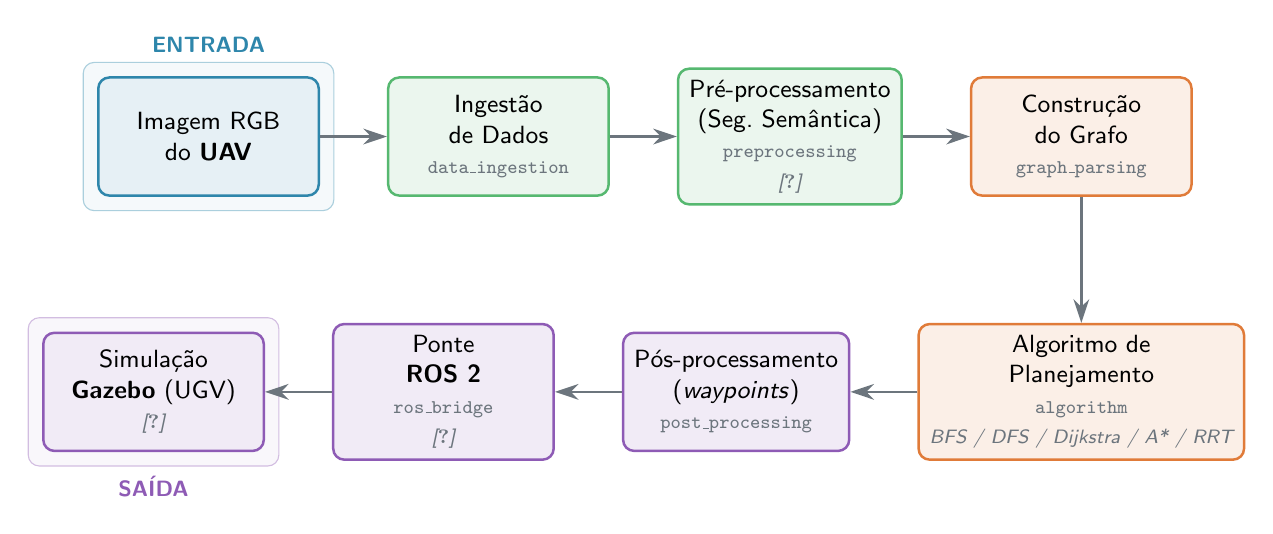
\begin{tikzpicture}[
        node distance=0.85cm and 0.85cm,
        every node/.append style={font=\small\sffamily}
    ]

        \node[pipelineBox=boxBlue]                    (img)
            {Imagem RGB \\ do \textbf{UAV}};
        \node[pipelineBox=boxGreen,  right=of img]    (ingest)
            {Ingestão \\ de Dados \\
             {\scriptsize\color{boxGray}\texttt{data\_\allowbreak{}ingestion}}};
        \node[pipelineBox=boxGreen,  right=of ingest] (pre)
            {Pré-processamento \\ (Seg.\ Semântica) \\
             {\scriptsize\color{boxGray}\texttt{preprocessing}} \\
             {\scriptsize\itshape\color{boxGray}\cite{junior2024_models}}};
        \node[pipelineBox=boxOrange, right=of pre]    (graph)
            {Construção \\ do Grafo \\
             {\scriptsize\color{boxGray}\texttt{graph\_\allowbreak{}parsing}}};

        \node[pipelineBox=boxOrange, below=1.6cm of graph] (algo)
            {Algoritmo de \\ Planejamento \\
             {\scriptsize\color{boxGray}\texttt{algorithm}} \\
             {\scriptsize\itshape\color{boxGray}BFS / DFS / Dijkstra / A* / RRT}};
        \node[pipelineBox=boxPurple, left=of algo]    (post)
            {Pós-processamento \\ (\textit{waypoints}) \\
             {\scriptsize\color{boxGray}\texttt{post\_\allowbreak{}processing}}};
        \node[pipelineBox=boxPurple, left=of post]    (bridge)
            {Ponte \\ \textbf{ROS 2} \\
             {\scriptsize\color{boxGray}\texttt{ros\_\allowbreak{}bridge}} \\
             {\scriptsize\itshape\color{boxGray}\cite{quigley2009}}};
        \node[pipelineBox=boxPurple, left=of bridge]  (gz)
            {Simulação \\ \textbf{Gazebo} (UGV) \\
             {\scriptsize\itshape\color{boxGray}\cite{koenig2004}}};

        \draw[pipelineArrow] (img)    -- (ingest);
        \draw[pipelineArrow] (ingest) -- (pre);
        \draw[pipelineArrow] (pre)    -- (graph);
        \draw[pipelineArrow] (graph.south) -- (algo.north);
        \draw[pipelineArrow] (algo)   -- (post);
        \draw[pipelineArrow] (post)   -- (bridge);
        \draw[pipelineArrow] (bridge) -- (gz);

        \node[font=\footnotesize\sffamily\bfseries, text=boxBlue,
              anchor=south, above=0.18cm of img.north]
            {ENTRADA};
        \node[font=\footnotesize\sffamily\bfseries, text=boxPurple,
              anchor=north, below=0.18cm of gz.south]
            {SAÍDA};

        \begin{scope}[on background layer]
            \node[draw=boxBlue!40, fill=boxBlue!5, rounded corners=4pt,
                  fit=(img), inner sep=5pt] {};
            \node[draw=boxPurple!40, fill=boxPurple!5, rounded corners=4pt,
                  fit=(gz), inner sep=5pt] {};
        \end{scope}

    \end{tikzpicture}}
    \caption{\textit{Pipeline} completo do sistema, da imagem RGB capturada pelo UAV até a simulação do movimento do UGV no Gazebo.}
    \label{fig:pipeline}
\end{figure}

\subsection{Diferenças em Relação ao PFC 2025}
\label{subsec:diferencas}

Em relação ao PFC 2025 \cite{camelo2025}, a arquitetura difere principalmente quanto à organização do código e ao acoplamento entre etapas: naquele trabalho, leitura de imagem, segmentação por cor, construção do grafo e execução dos algoritmos eram fortemente acopladas em \textit{scripts} sequenciais, o que tornava trabalhosa a substituição de qualquer uma das etapas. A Figura~\ref{fig:comparacao_arquitetura} resume as diferenças.

\begin{figure}[H]
    \centering
    \resizebox{0.95\textwidth}{!}{%
    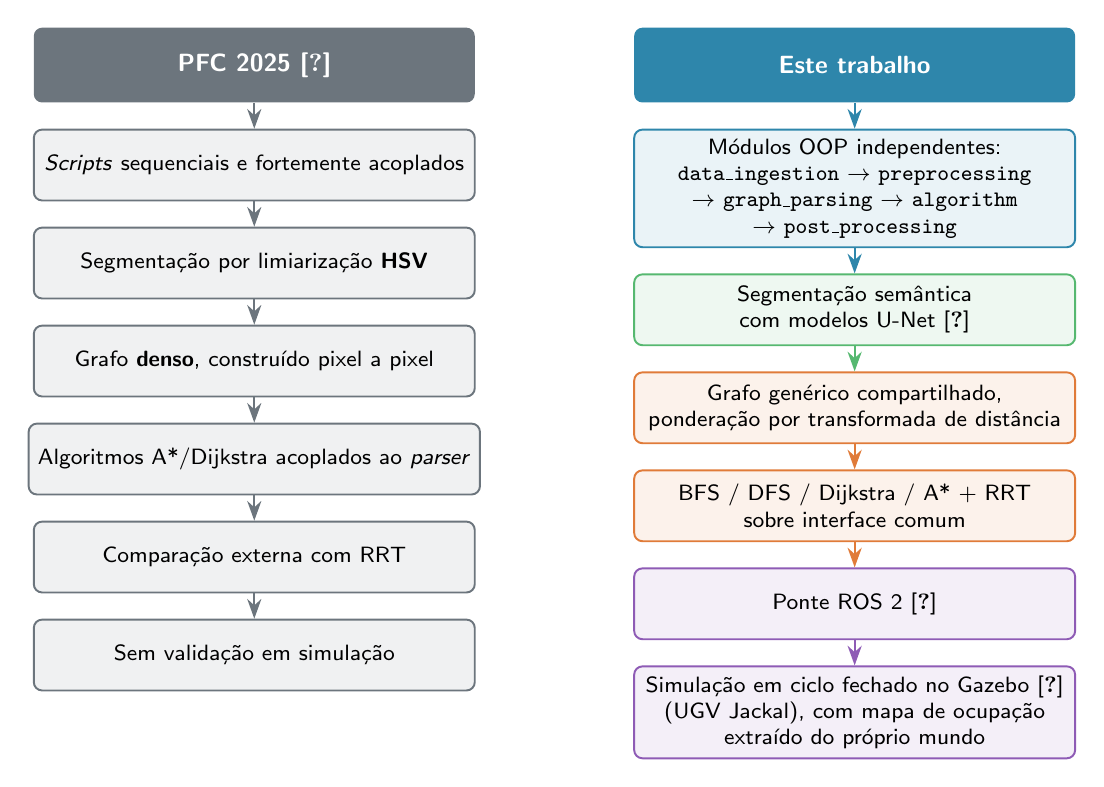
\begin{tikzpicture}[node distance=0.32cm]

        \node[compTitle=boxGray] (tA) {PFC 2025 \cite{camelo2025}};
        \node[compBox=boxGray, below=of tA] (a1)
            {\textit{Scripts} sequenciais e fortemente acoplados};
        \node[compBox=boxGray, below=of a1] (a2)
            {Segmentação por limiarização \textbf{HSV}};
        \node[compBox=boxGray, below=of a2] (a3)
            {Grafo \textbf{denso}, construído pixel a pixel};
        \node[compBox=boxGray, below=of a3] (a4)
            {Algoritmos A*/Dijkstra acoplados ao \textit{parser}};
        \node[compBox=boxGray, below=of a4] (a5)
            {Comparação externa com RRT};
        \node[compBox=boxGray, below=of a5] (a6)
            {Sem validação em simulação};

        \foreach \src/\dst in {tA/a1, a1/a2, a2/a3, a3/a4, a4/a5, a5/a6}{
            \draw[compArrow=boxGray] (\src) -- (\dst);
        }

        \node[compTitle=boxBlue, right=2.0cm of tA] (tB) {Este trabalho};
        \node[compBox=boxBlue, below=of tB] (b1)
            {Módulos OOP independentes:\\
             \texttt{data\_\allowbreak{}ingestion} $\to$ \texttt{preprocessing}\\
             $\to$ \texttt{graph\_\allowbreak{}parsing} $\to$ \texttt{algorithm}\\
             $\to$ \texttt{post\_\allowbreak{}processing}};
        \node[compBox=boxGreen, below=of b1] (b2)
            {Segmentação semântica\\ com modelos U-Net \cite{junior2024_models}};
        \node[compBox=boxOrange, below=of b2] (b3)
            {Grafo genérico compartilhado,\\ ponderação por transformada de distância};
        \node[compBox=boxOrange, below=of b3] (b4)
            {BFS / DFS / Dijkstra / A* + RRT\\ sobre interface comum};
        \node[compBox=boxPurple, below=of b4] (b5)
            {Ponte ROS 2 \cite{quigley2009}};
        \node[compBox=boxPurple, below=of b5] (b6)
            {Simulação em ciclo fechado no Gazebo \cite{koenig2004}\\ (UGV Jackal), com mapa de ocupação\\ extraído do próprio mundo};

        \draw[compArrow=boxBlue]   (tB) -- (b1);
        \draw[compArrow=boxBlue]   (b1) -- (b2);
        \draw[compArrow=boxGreen]  (b2) -- (b3);
        \draw[compArrow=boxOrange] (b3) -- (b4);
        \draw[compArrow=boxOrange] (b4) -- (b5);
        \draw[compArrow=boxPurple] (b5) -- (b6);

    \end{tikzpicture}}
    \caption{Comparativo da estrutura entre o PFC 2025 \cite{camelo2025} e este trabalho. Em destaque, na coluna da direita, os componentes desenvolvidos neste projeto: segmentação semântica, inclusão do RRT e simulação em ciclo fechado.}
    \label{fig:comparacao_arquitetura}
\end{figure}

% -- 3.2 -------------------------------------------------------------------
\section{Construção dos Grafos}
\label{sec:construcao_grafos}

A construção dos grafos toma como entrada o mapa de navegabilidade gerado pela segmentação (Seção~\ref{sec:mapa_navegabilidade}). O \textit{parser} identifica como vértices os pixels marcados como transitáveis e estabelece arestas entre vizinhos imediatos, conforme a conectividade escolhida.

Sobre a definição de grafo $G = (V, E)$ da Seção~2.3, adota-se neste projeto uma representação enriquecida, composta por:

\begin{itemize}
    \item \textbf{\textit{Node embeddings}} (atributos dos vértices): vetor $(x, y, p)$ para cada vértice, com as coordenadas espaciais $(x, y)$ do pixel e a penalidade de proximidade $p$, definida a seguir;
    \item \textbf{\textit{Edge index}} (lista de arestas): tensor de dimensão $(2, |E|)$ com os pares (origem, destino) de cada aresta, seguindo a convenção do PyTorch Geometric;
    \item \textbf{\textit{Edge embeddings}} (atributos das arestas): vetor $(w, \delta)$ para cada aresta, com o peso $w$ e o comprimento geométrico $\delta$ do passo, definidos a seguir.
\end{itemize}

Essa representação também tem uma vantagem prática: como os atributos dos vértices, a lista de arestas e os atributos das arestas ficam em três estruturas numéricas separadas, o grafo pode ser usado diretamente por bibliotecas de aprendizado em grafos, sem conversão adicional, o que deixa aberta a possibilidade de, em trabalhos futuros, aprender a função de custo em vez de defini-la manualmente.

\subsection{Função de Peso e Custo das Arestas}

Esta seção define a função de pesos $w : E \to \mathbb{R}_{\geq 0}$ introduzida na Seção~\ref{sec:caminhos_minimos}, que penaliza trajetórias próximas a obstáculos. Ela é construída em duas partes: uma penalidade associada a cada vértice e, a partir dela, o peso de cada aresta. Seja $d(v)$ a distância euclidiana, em pixels, de um vértice $v$ ao obstáculo mais próximo, obtida pela transformada de distância (\texttt{scipy.\allowbreak ndimage.\allowbreak distance\_\allowbreak{}\allowbreak transform\_\allowbreak{}\allowbreak edt}); sejam $r$ (\texttt{robot\_\allowbreak{}size}) a folga mínima exigida e $L$ (\texttt{weight\_\allowbreak{}limit}) o raio do campo de proximidade. A penalidade de um vértice é dada por

\[
p(v) =
\begin{cases}
\infty, & \text{se } d(v) \leq r \quad \text{(vértice bloqueado)},\\[0.3em]
L - d(v), & \text{se } r < d(v) < L,\\[0.3em]
0, & \text{se } d(v) \geq L.
\end{cases}
\]

Vértices a menos de $r$ pixels de um obstáculo são descartados, porque o veículo não caberia ali: $r$ representa, em pixels, o raio do robô mais uma margem de segurança. Entre $r$ e $L$, a penalidade cresce linearmente à medida que o vértice se aproxima do obstáculo, o que torna os caminhos rentes às bordas mais caros sem proibi-los. A partir de $L$ pixels de distância, considera-se que não há mais influência do obstáculo e a penalidade é nula. O parâmetro $L$ controla, portanto, o quanto o planejador prefere andar pelo meio dos corredores livres.

Para uma aresta $e = (u, v)$, que vai do vértice $u$ para o vértice $v$, seja $\delta(e) \in \{1, \sqrt{2}\}$ o comprimento geométrico do passo, em pixels, sendo $1$ para vizinhos ortogonais e $\sqrt{2}$ para diagonais. O peso da aresta soma a esse comprimento a penalidade do vértice de chegada:

\[
w(e) = \delta(e) + p(v).
\]

Os dois valores, $w(e)$ e $\delta(e)$, são armazenados no \textit{edge embedding}. O peso $w(e)$ é o utilizado na busca ponderada (Dijkstra e A*) e é com ele que se calcula o custo $\ell(P)$ de um caminho, segundo a definição apresentada na Seção~\ref{sec:caminhos_minimos}. Esse peso penaliza a proximidade de obstáculos e faz com que os caminhos se afastem das regiões de risco. Como a penalidade depende apenas do vértice de chegada, $w(u, v)$ e $w(v, u)$ podem ser diferentes, o que explica por que o grafo é direcionado (Seção~2.3).

Como consequência dessa definição, o custo total $\ell(P)$ reportado para um caminho ponderado não tem unidade de comprimento: ele mistura pixels percorridos com penalizações de proximidade. Por isso, as tabelas de resultados reportam também a distância percorrida pelo caminho, em pixels, que é a soma dos comprimentos geométricos $\delta(e_i)$ das suas arestas. Havendo correspondência conhecida entre o tamanho do pixel e os metros que ele representa (o GSD, Seção~\ref{sec:gsd}), essa distância pode ser convertida exatamente no comprimento do caminho em metros, multiplicando-a pelo GSD.

\subsection{Eficiência da Construção}

Os principais aprimoramentos em relação ao PFC 2025 \cite{camelo2025} na etapa de construção são:

\begin{itemize}
    \item \textbf{Ponderação por transformada de distância}: a penalidade de cada vértice é obtida em uma única passagem pela imagem com \texttt{scipy.\allowbreak ndimage.\allowbreak distance\_\allowbreak{}\allowbreak transform\_\allowbreak{}\allowbreak edt}, substituindo a verificação iterativa pixel a pixel do projeto anterior, na qual, para cada pixel, percorria-se a sua vizinhança em busca de obstáculos;
    \item \textbf{Construção vetorizada}: as arestas são construídas com operações NumPy sobre a matriz inteira, evitando laços Python sobre cada pixel. Em um grafo de alguns milhões de arestas, o tempo de construção com operações vetorizadas é da ordem de cem vezes menor que o obtido com laços sobre cada pixel.
\end{itemize}

A função \texttt{build\_\allowbreak{}grid\_\allowbreak{}graph()}, em \texttt{graph\_\allowbreak{}parsing/\allowbreak{}\_\allowbreak{}grid\_\allowbreak{}utils.py}, é compartilhada entre o \texttt{GridImageGraphParser}, usado para imagens com cores fixas como o mapa de navegabilidade adotado em \cite{junior2025_rrt}, e o \texttt{SegmentedImageGraphParser}, usado para imagens segmentadas semanticamente.

% -- 3.3 -------------------------------------------------------------------
\section{Inclusão do Algoritmo RRT}
\label{sec:impl_rrt}

O RRT (Seção~\ref{sec:rrt}) foi adicionado ao módulo \texttt{algorithm} sob a mesma interface \texttt{PathAlgorithm} dos demais planejadores, sendo registrado na fábrica junto com BFS, DFS, Dijkstra e A*. A implementação segue de perto a referência de Junior \cite{junior2025_rrt}, porém integrada à arquitetura do projeto:

\begin{itemize}
    \item \textbf{Espaço contínuo sobre o mapa.} Ao contrário dos algoritmos de busca em grafos, que operam sobre a estrutura discreta, o RRT opera em coordenadas contínuas de pixel. O espaço livre, as coordenadas de origem e destino e a folga aos obstáculos são obtidos a partir do próprio \texttt{Graph}: um pixel é livre quando é um vértice transitável e está suficientemente afastado de obstáculos, ou seja, quando a sua penalidade é finita segundo a transformada de distância. Assim, o RRT respeita a mesma folga (\texttt{robot\_\allowbreak{}size}) dos demais algoritmos, o que coloca todos os planejadores nas mesmas condições;
    \item \textbf{Verificação de colisão.} Segue a convenção de \cite{junior2025_rrt}: amostram-se cerca de 100 pontos ao longo do segmento entre duas posições, exigindo-se que todos recaiam sobre o espaço livre. A amostragem é feita de forma paramétrica, o que evita a divisão por zero da implementação de referência em segmentos verticais;
    \item \textbf{Compatibilidade com o pós-processamento.} Cada \textit{waypoint} da árvore é associado ao vértice do grafo mais próximo, de modo que os pós-processadores existentes, de geração de \textit{waypoints} e de desenho sobre a imagem, funcionem sem alteração. O custo reportado é o comprimento geométrico do caminho, e não o custo ponderado dos algoritmos de busca;
    \item \textbf{Parâmetros.} \textit{Step size} (padrão 20 px), número máximo de iterações, taxa de amostragem do objetivo e semente do gerador de números pseudoaleatórios, esta última para permitir reprodutibilidade. São expostos tanto na linha de comando quanto na interface gráfica de teste.
\end{itemize}

% -- 3.4 -------------------------------------------------------------------
\section{Implementação da Segmentação Semântica}
\label{sec:impl_segmentacao}

O módulo \texttt{preprocessing} executa a inferência dos modelos de \cite{junior2024_models} (Seção~\ref{sec:ia}). Cada modelo é uma rede U-Net \cite{ronneberger2015} com um \textit{backbone} convolucional (ResNet 50/101, EfficientNet-B4/B5 ou MobileNet V2), que produz, para cada pixel, uma distribuição sobre as 23 classes do \emph{Semantic Drone Dataset}. O processamento compreende:

\begin{enumerate}
    \item \textbf{Pré-processamento da imagem.} Conversão para RGB, normalização estatística com a média e o desvio-padrão da ImageNet, coerentes com o treinamento, e, como o codificador reduz a resolução por um fator de 32, preenchimento (\textit{padding}) das bordas até o múltiplo de 32 mais próximo, recortado após a inferência. Sem esse preenchimento, as dimensões da saída do decodificador não coincidem com as da entrada e a rede falha;
    \item \textbf{Inferência e agrupamento de classes.} A classe de cada pixel é obtida pelo índice de maior probabilidade (\textit{argmax}); as classes são então agrupadas em transitável e não transitável, considerando-se transitáveis as classes de solo (\textit{paved-area}, \textit{dirt}, \textit{grass}, \textit{gravel}), segundo critérios herdados de \cite{junior2024};
    \item \textbf{Pós-processamento opcional da máscara.} Filtragem por confiança da predição, redimensionamento e limpeza morfológica, que consiste em fechamento e abertura seguidos da remoção de componentes conexos pequenos. O fechamento preenche buracos internos da máscara, a abertura elimina ruído isolado e a remoção de componentes descarta ilhas transitáveis desconectadas da região principal. Estas etapas são configuráveis e vêm desativadas, de modo que a configuração de origem entregue a máscara bruta do modelo;
    \item \textbf{Geração do mapa de navegabilidade.} Aplicação da paleta de cores de \cite{junior2025_rrt}, produzindo o mapa consumido pelo \texttt{graph\_\allowbreak{}parsing}.
\end{enumerate}

A seleção do modelo em tempo de execução é um hiperparâmetro do \textit{pipeline}, o que permite trocar o \textit{backbone} sem alterar os demais módulos.

% -- 3.5 -------------------------------------------------------------------
\section{Integração com ROS 2 e Simulação no Gazebo}
\label{sec:ros_integracao}

Esta etapa liga o planejamento à execução do movimento e é composta por duas atividades: a publicação do caminho pelo \textit{pipeline} de planejamento e o seu recebimento pelo robô simulado. A Figura~\ref{fig:ros_fluxo} mostra os nós ROS 2 envolvidos e os tópicos pelos quais eles se comunicam. Como o emissor de cada tópico não precisa conhecer o receptor (Seção~\ref{sec:ros2}), o UGV simulado pode ser substituído por um veículo real sem alterar o planejamento, desde que este publique e assine os mesmos tópicos.

\begin{figure}[H]
    \centering
    \resizebox{\textwidth}{!}{%
    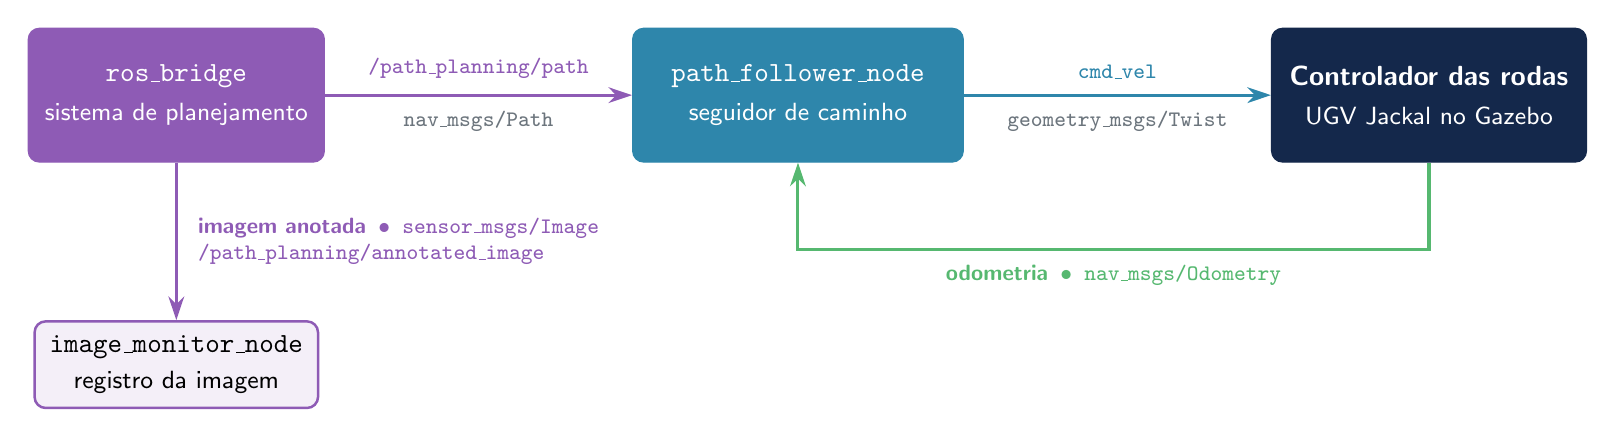
\begin{tikzpicture}[
        rosNode/.style={
            rectangle, rounded corners=4pt, fill=#1, draw=#1,
            minimum height=1.7cm, align=center, inner sep=6pt,
            font=\sffamily, text=white
        },
        rosArrow/.style={
            -{Stealth[length=3mm, width=2mm]}, line width=1.1pt, draw=#1
        },
        topicName/.style={font=\footnotesize\ttfamily\bfseries, text=#1},
        msgType/.style={font=\footnotesize\ttfamily, text=boxGray}
    ]

        \node[rosNode=boxPurple, minimum width=3.6cm] (bridge)
            {\textbf{\texttt{ros\_bridge}}\\[2pt] {\small sistema de planejamento}};
        \node[rosNode=boxBlue, minimum width=4.2cm, right=3.9cm of bridge] (follower)
            {\textbf{\texttt{path\_follower\_node}}\\[2pt] {\small seguidor de caminho}};
        \node[rosNode=rosNavy, minimum width=4.0cm, right=3.9cm of follower] (ctrl)
            {\textbf{Controlador das rodas}\\[2pt] {\small UGV Jackal no Gazebo}};
        \node[rectangle, rounded corners=4pt, draw=boxPurple, fill=boxPurple!10,
              line width=0.9pt, minimum width=3.6cm, minimum height=1.1cm,
              align=center, font=\sffamily, below=2.0cm of bridge] (monitor)
            {\textbf{\texttt{image\_monitor\_node}}\\[1pt] {\small registro da imagem}};

        % caminho planejado
        \draw[rosArrow=boxPurple] (bridge.east) -- (follower.west)
            node[midway, above=2pt, topicName=boxPurple] {/path\_planning/path}
            node[midway, below=2pt, msgType] {nav\_msgs/Path};

        % comandos de velocidade
        \draw[rosArrow=boxBlue] (follower.east) -- (ctrl.west)
            node[midway, above=2pt, topicName=boxBlue] {cmd\_vel}
            node[midway, below=2pt, msgType] {geometry\_msgs/Twist};

        % realimentacao por odometria
        \draw[rosArrow=boxGreen] (ctrl.south) -- ++(0,-1.1)
            -| (follower.south)
            node[pos=0.25, below=2pt, font=\footnotesize\sffamily\bfseries, text=boxGreen]
            {odometria \,$\bullet$\, \texttt{nav\_msgs/Odometry}};

        % imagem anotada
        \draw[rosArrow=boxPurple] (bridge.south) -- (monitor.north)
            node[midway, right=4pt, align=left, font=\footnotesize\sffamily\bfseries, text=boxPurple]
            {imagem anotada \,$\bullet$\, \texttt{sensor\_msgs/Image}\\
             {\mdseries\ttfamily /path\_planning/annotated\_image}};

    \end{tikzpicture}}
    \caption{Nós ROS 2 e tópicos envolvidos na execução da trajetória no Gazebo. A ponte \texttt{ros\_\allowbreak{}bridge} publica o caminho, que o \texttt{path\_\allowbreak{}follower\_\allowbreak{}node} converte em comandos de velocidade para o controlador das rodas do Jackal; a odometria fecha a malha de controle. A imagem anotada é registrada pelo \texttt{image\_\allowbreak{}monitor\_\allowbreak{}node}. No Jackal simulado, os tópicos de comando e de odometria recebem o prefixo do robô (\texttt{j100\_\allowbreak{}0000/\allowbreak{}cmd\_\allowbreak{}vel} e \texttt{j100\_\allowbreak{}0000/\allowbreak{}platform/\allowbreak{}odom/\allowbreak{}filtered}).}
    \label{fig:ros_fluxo}
\end{figure}

\subsection{Publicação: a ponte \texttt{ros\_\allowbreak{}bridge}}

O módulo \texttt{post\_\allowbreak{}processing} foi estendido com uma ponte ROS 2 (\texttt{ros\_\allowbreak{}bridge}) que publica mensagens em dois tópicos: um com a imagem aérea anotada com a trajetória (\texttt{sensor\_\allowbreak{}msgs/\allowbreak{}Image}) e outro com o caminho, na forma de uma sequência de poses (\texttt{nav\_\allowbreak{}msgs/\allowbreak{}Path}). Como os \textit{waypoints} são expressos em coordenadas de pixel, a ponte os converte para metros pelas expressões da Seção~\ref{sec:gsd}, aplicando o fator de escala e a inversão do eixo vertical. Utiliza-se a política de QoS \textit{transient local} discutida na Seção~\ref{sec:ros2}. Antes de publicar, a ponte aguarda até 3 s que os assinantes do robô sejam descobertos e, depois de publicar, permanece ativa por um breve intervalo, para que a mensagem retida seja efetivamente entregue antes do encerramento do processo.

\subsection{Consumo: o pacote \texttt{ugv\_\allowbreak{}bridge} e o UGV simulado}

No robô, um pacote ROS 2 (\texttt{ugv\_\allowbreak{}bridge}) reúne os nós que fazem o UGV simulado percorrer a trajetória:

\begin{itemize}
    \item \texttt{path\_\allowbreak{}follower\_\allowbreak{}node}: seguidor de \textit{waypoints} para um robô de tração diferencial, detalhado a seguir;
    \item \texttt{tf\_\allowbreak{}odom\_\allowbreak{}bridge\_\allowbreak{}node}: quando necessário, recebe a transformação de pose (TF) do robô e a publica novamente, convertida em uma mensagem de odometria (\texttt{nav\_\allowbreak{}msgs/\allowbreak{}Odometry}), que é o formato esperado pelo seguidor. Esse nó é desnecessário quando o veículo já publica odometria própria, como é o caso do Jackal, e por isso pode ser desativado por parâmetro;
    \item \texttt{image\_\allowbreak{}monitor\_\allowbreak{}node}: registra a imagem anotada publicada pela ponte, servindo como verificação de que a informação visual também chegou ao lado do robô.
\end{itemize}

O \texttt{path\_\allowbreak{}follower\_\allowbreak{}node} implementa um seguidor de \textit{waypoints} simples. A cada ciclo de controle, ele lê a pose atual $(x, y, \theta)$ da odometria, toma o \textit{waypoint} corrente $(x_t, y_t)$ e calcula o erro de proa
\[
e_\theta = \mathrm{atan2}\big(\sin(\theta_d - \theta),\ \cos(\theta_d - \theta)\big),
\qquad
\theta_d = \mathrm{atan2}(y_t - y,\ x_t - x),
\]
onde a forma com seno e cosseno garante que o erro fique no intervalo $(-\pi, \pi]$, evitando que o robô gire pelo lado mais longo. Os comandos de velocidade, publicados no tópico de comando do robô como mensagens do tipo \texttt{geometry\_\allowbreak{}msgs/\allowbreak{}Twist}, são
\[
\omega = \mathrm{sat}\big(2\,e_\theta,\ \omega_{\max}\big),
\qquad
v = v_{\text{cruzeiro}} \cdot \max\left(0,\ 1 - \frac{|e_\theta|}{\pi/2}\right),
\]
isto é, a velocidade angular é proporcional ao erro de proa, limitada a um valor máximo, e a velocidade linear é reduzida proporcionalmente ao desalinhamento, anulando-se quando o robô precisa girar mais de noventa graus. Esse acoplamento evita que o veículo avance na direção errada enquanto ainda está se alinhando. Um \textit{waypoint} é considerado alcançado quando a distância até ele fica abaixo de uma tolerância, de 0,12 m para os pontos intermediários e de 0,15 m para o ponto final. A velocidade angular máxima é $\omega_{\max} = 1{,}0$ rad/s, e a velocidade de cruzeiro é $v_{\text{cruzeiro}} = 0{,}4$ m/s.

Como plataforma de demonstração, adotou-se o UGV Clearpath Jackal simulado no Gazebo, iniciado por um \textit{launch file} de integração que sobe a simulação e os nós do \texttt{ugv\_\allowbreak{}bridge}. Nessa configuração, a odometria filtrada é fornecida por um filtro de Kalman estendido (EKF) que funde a odometria das rodas e a IMU (Seção~\ref{sec:odometria}). O fluxo completo é, portanto: o \textit{pipeline} planeja e publica o caminho, o \texttt{path\_\allowbreak{}follower\_\allowbreak{}node} converte o caminho em comandos de velocidade, e o Jackal percorre a trajetória no Gazebo até o destino.

A Figura~\ref{fig:gazebo_jackal} mostra o veículo simulado no mundo \textit{warehouse}, com o painel de teleoperação publicando no mesmo tópico de comando de velocidade usado pela integração. Essa imagem foi obtida com a interface gráfica tridimensional do Gazebo aberta manualmente, com renderização por \textit{software}, em uma sessão interativa usada para inspecionar o mundo e testar a teleoperação. Como explicado na Seção~\ref{sec:lim_sim}, essa interface não funcionou de forma confiável no ambiente utilizado, e por isso os ensaios de percurso do Capítulo~\ref{cap:resultados} foram executados sem ela, com o simulador em modo \textit{headless}.

\begin{figure}[H]
    \centering
    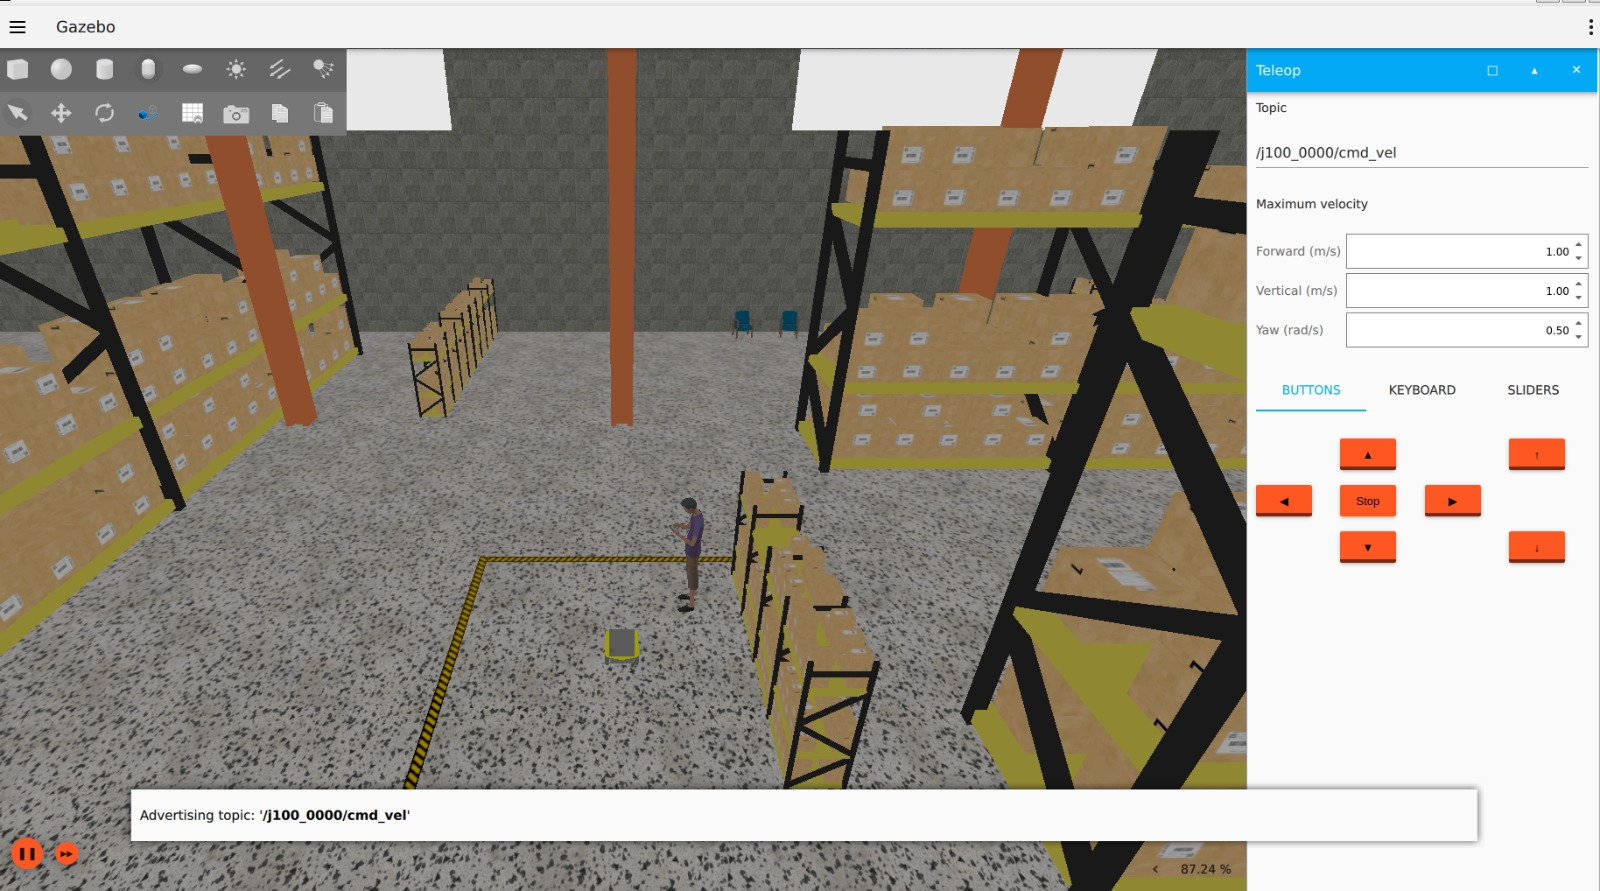
\includegraphics[width=0.95\textwidth]{figuras/gazebo_jackal.jpg}
    \caption{UGV Clearpath Jackal simulado no mundo \textit{warehouse} do Gazebo. À direita, o painel de teleoperação publicando comandos de velocidade (\texttt{geometry\_\allowbreak{}msgs/\allowbreak{}Twist}) no tópico \texttt{cmd\_\allowbreak{}vel} consumido pela integração.}
    \label{fig:gazebo_jackal}
\end{figure}

% -- 3.6 -------------------------------------------------------------------
\section{Geração do Mapa de Ocupação a partir do Mundo Simulado}
\label{sec:mapa_ocupacao}

Nos primeiros ensaios de simulação, o caminho era planejado sobre uma imagem (sintética ou aérea) e depois publicado para o robô no Gazebo. Isso deixava em aberto uma questão de referencial: a imagem e o mundo simulado são cenários distintos, de modo que a correspondência entre eles dependia inteiramente do ajuste manual do fator de escala e da origem. Quando esses valores não eram exatos, o robô percorria uma trajetória com a forma correta, mas deslocada ou fora de escala em relação aos obstáculos do mundo, conforme discutido na Seção~\ref{subsec:alinhamento}.

Para eliminar essa fonte de erro, foi desenvolvido um conversor (\texttt{scripts/\allowbreak{}\allowbreak gazebo\_\allowbreak{}\allowbreak world\_\allowbreak{}\allowbreak to\_\allowbreak{}\allowbreak occupancy.py}) que lê o arquivo SDF do mundo do Gazebo e produz uma vista superior bidimensional dele, no mesmo formato de mapa de navegabilidade consumido pelo \texttt{graph\_\allowbreak{}parsing} (Seção~\ref{sec:mapa_navegabilidade}). O procedimento é:

\begin{enumerate}
    \item \textbf{Percurso da árvore do mundo.} São visitados todos os modelos definidos diretamente no arquivo e todos os modelos incluídos por referência, resolvidos tanto em diretórios locais quanto no cache de modelos baixados do repositório de modelos do simulador;
    \item \textbf{Composição de poses.} Cada elemento de colisão tem a sua pose composta com as poses do elo (\textit{link}) e do modelo que o contêm, resultando em uma transformação homogênea que leva a geometria local para o referencial do mundo;
    \item \textbf{Rasterização da geometria.} Caixas e cilindros são projetados diretamente no plano horizontal. Malhas trianguladas no formato STL têm seus triângulos transformados e projetados; triângulos quase horizontais, que correspondem a pisos e tetos, são descartados por um critério de inclinação, de modo que apenas geometria de parede se torne obstáculo. Elementos que não podem ser resolvidos, como planos infinitos ou malhas em formatos não suportados, são ignorados com aviso, e não viram obstáculo;
    \item \textbf{Escrita do mapa.} A área livre recebe a cor transitável convencionada e os obstáculos recebem preto. O programa imprime os valores exatos de resolução em metros por pixel e de origem em metros a serem passados ao \textit{pipeline}, de forma que o caminho planejado caia exatamente sobre o referencial do mundo.
\end{enumerate}

O mundo \textit{warehouse}, fornecido com o simulador do Jackal, representa um galpão fechado de cerca de $30 \times 50$ m, com prateleiras longas e paralelas, paredes internas e corredores. O mapa de ocupação gerado para ele é mostrado na Figura~\ref{fig:mapa_ocupacao}. A consequência prática é que o planejamento passa a ocorrer sobre a geometria real do ambiente em que o veículo vai se mover, com correspondência métrica exata, o que separa claramente dois tipos de erro que antes se confundiam: erros do planejador e erros de alinhamento entre referenciais.

\begin{figure}[H]
    \centering
    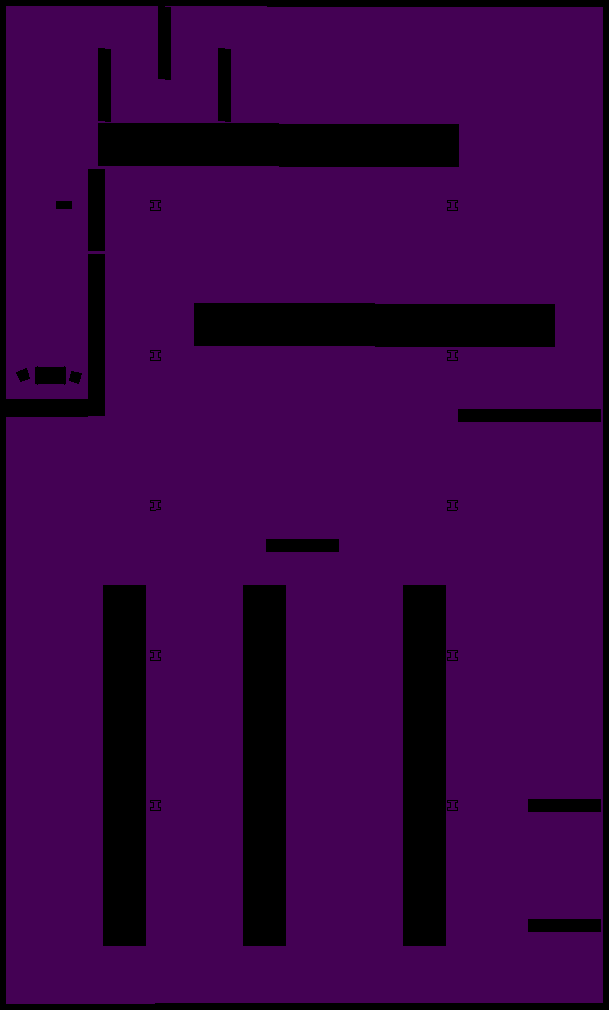
\includegraphics[width=0.52\textwidth]{figuras/mapa_ocupacao.png}
    \caption{Mapa de ocupação gerado automaticamente a partir da descrição SDF do mundo \textit{warehouse} do Gazebo. Em roxo, a área livre, na cor convencionada para regiões transitáveis; em preto, a geometria de colisão projetada no plano horizontal. Resolução de 0,05 m por pixel.}
    \label{fig:mapa_ocupacao}
\end{figure}

% -- 3.7 -------------------------------------------------------------------
\section{Pós-processamento e Formato de Saída}

Além da ponte ROS 2, o módulo \texttt{post\_\allowbreak{}processing} mantém dois processadores. O \texttt{SimpleWaypointProcessor} converte a sequência de vértices em \textit{waypoints} com coordenadas $(x, y)$, ângulo de proa $\theta$ e tipo de movimento, encapsulados na \textit{dataclass} \texttt{RobotPath}. O ângulo de proa de cada ponto é o da direção para o ponto seguinte, o que dá ao seguidor uma referência de orientação além da posição. O \texttt{ImageDrawingPostProcessor} desenha os caminhos sobre a imagem original, com cores distintas por algoritmo e marcadores de início e fim, e é a origem das figuras comparativas do Capítulo~\ref{cap:resultados}.

% -- 3.8 -------------------------------------------------------------------
\section{Coleta dos Dados e Ambiente Experimental}
\label{sec:ambiente}

Para os experimentos, são utilizadas imagens RGB de alta resolução obtidas por drone, em cenários representativos de operação do UGV, com caminhos pavimentados, vegetação, praças e obstáculos diversos, incluindo imagens da Quinta da Boa Vista e do Outeiro da Glória, no Rio de Janeiro. Todas as imagens aéreas apresentadas no Capítulo~\ref{cap:resultados} são do Outeiro da Glória, área urbana com a igreja de mesmo nome, praças pavimentadas com pedras, ruas estreitas, edificações, veículos estacionados e vegetação. Elas foram capturadas por um drone DJI Mavic 3T com a câmera apontada para baixo (vista nadiral). A imagem usada no percurso simulado da Seção~\ref{sec:res_gazebo}, por exemplo, tem $4000 \times 3000$ pixels e, segundo os seus metadados, foi capturada em 26 de junho de 2024, a cerca de 41 m acima do ponto de decolagem, com a câmera inclinada a $-90^\circ$, isto é, exatamente na vertical. Os modelos de segmentação adotados já foram treinados em \cite{junior2024_models} sobre o \emph{Semantic Drone Dataset} \cite{drone_dataset} e são aqui avaliados sobre essas imagens reais, ou seja, em cenários diferentes daqueles em que foram treinados. Além das imagens aéreas, utiliza-se o mapa de ocupação do mundo \textit{warehouse}, gerado conforme a Seção~\ref{sec:mapa_ocupacao}.

Os ensaios de segmentação e de planejamento foram executados em duas máquinas. Os resultados de segmentação da Seção~\ref{sec:res_segmentacao} foram obtidos com aceleração em GPU integrada de arquitetura Apple Silicon. Os resultados de planejamento da Seção~\ref{sec:res_algoritmos} sobre o mapa de ocupação e os ensaios de simulação foram obtidos em processador Intel Core i7-1265U com 16 GB de memória, sem uso de GPU. Essas etapas não envolvem inferência de rede neural, com uma exceção: no percurso sobre imagem aérea, a segmentação foi feita nessa mesma máquina, com o modelo MobileNet V2 executado na CPU. A simulação foi executada em ROS 2 Humble e Gazebo sobre Ubuntu 22.04 em WSL2, configuração cujas limitações são discutidas na Seção~\ref{sec:limitacoes}.

% ======================================================================
\chapter{RESULTADOS E DISCUSSÃO}
\label{cap:resultados}
% ======================================================================

Neste capítulo, apresentamos e discutimos os resultados obtidos. As três primeiras seções tratam, respectivamente, dos modelos de segmentação, dos algoritmos de planejamento e da execução da trajetória no simulador. A última seção reúne as limitações encontradas e as dificuldades que impediram o cumprimento integral do planejamento inicial.

% -- 4.1 -------------------------------------------------------------------
\section{Comparação dos Modelos de Segmentação}
\label{sec:res_segmentacao}

A Tabela~\ref{tab:comparacao_modelos} reúne, para os modelos com métricas divulgadas em \cite{junior2024_models}, a mIoU e a acurácia sobre imagens de teste do \emph{Semantic Drone Dataset}, além da fração de área classificada como transitável e do tempo de inferência medidos neste trabalho sobre uma imagem aérea do Outeiro da Glória, redimensionada para $1024 \times 768$ pixels e mostrada na Figura~\ref{fig:segmentacao}. A implementação suporta ainda o \textit{backbone} MobileNet V2, aqui omitido da comparação quantitativa por não haver métricas de referência divulgadas.

\begin{table}[H]
    \centering
    \caption{Comparação dos modelos de segmentação. As colunas mIoU e acurácia são as divulgadas em \cite{junior2024_models}; a área transitável e o tempo de inferência foram medidos neste trabalho, sobre imagem de $1024 \times 768$ pixels, com aceleração em GPU integrada.}
    \label{tab:comparacao_modelos}
    \begin{tabular}{lcccc}
        \toprule
        \textbf{Modelo} & \textbf{mIoU} & \textbf{Acurácia} & \textbf{Área transit.\ (\%)} & \textbf{Tempo (s)} \\
        \midrule
        ResNet~50        & 0,3933 & 0,8244 & 65,5 & 0,72 \\
        ResNet~101       & 0,4032 & 0,8720 & 67,5 & 0,52 \\
        EfficientNet-B4  & 0,5012 & 0,9120 & 61,1 & 0,71 \\
        EfficientNet-B5  & 0,4819 & 0,9025 & 69,4 & 0,57 \\
        \bottomrule
    \end{tabular}
\end{table}

Os modelos EfficientNet apresentam as melhores métricas de referência, com destaque para o EfficientNet-B4, de maior mIoU (0,5012). Os tempos de inferência são todos inferiores a um segundo na resolução avaliada, sem diferença expressiva entre os \textit{backbones}, o que torna a mIoU o principal critério de escolha.

A coluna de área transitável é a única medida obtida sobre as imagens deste trabalho, e não sobre as imagens de teste do \emph{Semantic Drone Dataset}. Ela indica a fração da imagem que cada modelo considerou navegável. Não existe um valor correto conhecido para essas imagens, já que elas não são anotadas, mas a dispersão entre os modelos, de 61,1\% a 69,4\%, mostra que a escolha do \textit{backbone} altera de forma perceptível o espaço livre entregue ao planejador. Um modelo mais permissivo produz um grafo maior e pode incluir como transitáveis regiões de risco; um modelo mais conservador reduz o espaço de busca e pode fechar corredores estreitos. O EfficientNet-B4, de maior mIoU, é também o mais conservador dos quatro, o que é coerente com uma segmentação mais criteriosa das bordas entre classes.

A Figura~\ref{fig:segmentacao} mostra, para o EfficientNet-B4, a máscara de área transitável sobreposta à imagem de entrada, uma vista aérea do adro da igreja do Outeiro da Glória, cuja cobertura de planta octogonal aparece à direita da imagem. O pátio pavimentado e a vegetação rasteira são corretamente identificados como transitáveis, ao passo que a igreja, as demais edificações, as árvores densas e os veículos são excluídos. As bordas acompanham os limites reais das estruturas, inclusive em regiões sombreadas, que eram a principal dificuldade da limiarização de cor usada no PFC 2025.

\begin{figure}[H]
    \centering
    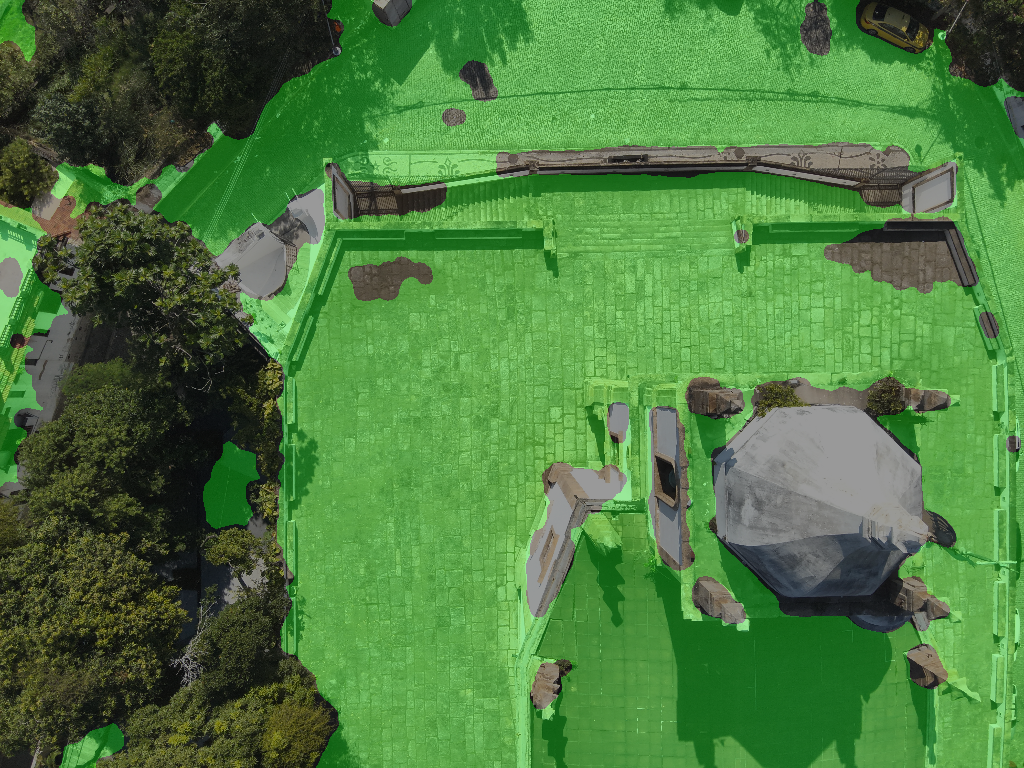
\includegraphics[width=0.95\textwidth]{figuras/segmentacao_b4.png}
    \caption{Segmentação com o modelo EfficientNet-B4 sobre imagem aérea do Outeiro da Glória, Rio de Janeiro ($1024 \times 768$ pixels): em verde, a região classificada como transitável, sobreposta à imagem de entrada.}
    \label{fig:segmentacao}
\end{figure}

% -- 4.2 -------------------------------------------------------------------
\section{Desempenho dos Algoritmos de Planejamento}
\label{sec:res_algoritmos}

\subsection{Comparação sobre Imagem Aérea Segmentada}

A Tabela~\ref{tab:comparacao_algoritmos} compara os cinco algoritmos sobre o mesmo grafo, gerado a partir de uma imagem aérea do Outeiro da Glória redimensionada para $1000 \times 750$ pixels, com cerca de $4{,}4 \times 10^5$ vértices e $3{,}3 \times 10^6$ arestas, e com os mesmos pontos de origem e destino. Para os algoritmos de busca, o custo reportado é o custo $\ell(P)$ do caminho $P$ devolvido, calculado com os pesos $w$ que penalizam a proximidade de obstáculos (Seção~\ref{sec:construcao_grafos}); para o Dijkstra e o A*, que são ótimos, esse valor é o custo do caminho mínimo, $\ell(P^\ast)$. Para o RRT, o valor reportado é o comprimento geométrico do caminho. A coluna de vértices dá o número $k+1$ de vértices do caminho, ou seja, o seu comprimento $k$ acrescido de um (Seção~\ref{sec:caminhos_minimos}).

\begin{table}[H]
    \centering
    \caption{Comparação dos algoritmos sobre o mesmo mapa do Outeiro da Glória ($1000 \times 750$ pixels; mesmos pontos de início e fim). Na coluna Custo, o valor do RRT é o comprimento geométrico do caminho, que não é comparável ao custo ponderado $\ell(P)$ dos demais algoritmos. A quarta coluna traz o número de vértices explorados pelos algoritmos de busca e o número de iterações do RRT.}
    \label{tab:comparacao_algoritmos}
    \small
    \setlength{\tabcolsep}{5pt}
    \begin{tabular}{lrrrrr}
        \toprule
        \textbf{Algoritmo}
            & \shortstack[r]{\textbf{Vértices}\\\textbf{($k+1$)}}
            & \shortstack[r]{\textbf{Custo}\\\textbf{$\ell(P)$}}
            & \shortstack[r]{\textbf{Vért. expl.}\\\textbf{ou iter.}}
            & \shortstack[r]{\textbf{Tempo}\\\textbf{(s)}}
            & \shortstack[r]{\textbf{Distância}\\\textbf{(px)}} \\
        \midrule
        BFS      &    351 &    12.838,8 & 179.546 & 0,131 &    398,0 \\
        DFS      & 65.282 & 1.314.372,7 & 248.479 & 0,159 & 92.241,7 \\
        Dijkstra &    879 &     1.462,2 & 228.525 & 0,392 &    990,7 \\
        A*       &    879 &     1.462,2 & 203.472 & 0,426 &    990,7 \\
        RRT      &     30 &       931,6 &     289 & 0,010 &    931,8 \\
        \bottomrule
    \end{tabular}
\end{table}

Os resultados são coerentes com a teoria e com o observado no PFC 2025 \cite{camelo2025}:

\begin{itemize}
    \item \textbf{A* e Dijkstra} produzem caminhos ótimos de mesmo custo, $\ell(P^\ast) = 1.462{,}2$, mas o A* explora menos vértices, 203.472 contra 228.525, graças à heurística, o que confirma a preferência pelo A* já apontada no PFC 2025. Apesar de explorar cerca de 11\% menos vértices, o A* não foi mais rápido em tempo de execução neste ensaio, pelo motivo discutido na Seção~\ref{sec:caminhos_minimos}: o custo por vértice expandido é maior, porque cada vizinho exige o cálculo da heurística euclidiana. A vantagem do A* cresce quando o grafo é maior ou quando a heurística é mais informativa em relação ao formato do espaço livre;
    \item \textbf{A BFS} encontra o caminho com menor número de arestas, o que corresponde à menor distância percorrida, de 398,0 px, porém, por ignorar a penalização por proximidade a obstáculos, conforme antecipado na Seção~\ref{sec:caminhos_minimos}, apresenta um custo ponderado muito maior que o dos algoritmos ótimos, de 12.838,8. Esses valores mostram a diferença entre os dois critérios: o caminho mais curto passa rente aos obstáculos, enquanto o caminho de menor custo ponderado é cerca de duas vezes e meia mais longo, mas se mantém afastado deles;
    \item \textbf{A DFS} confirma seu caráter não ótimo, produzindo um caminho de 65.282 vértices, com distância percorrida cerca de cem vezes maior que a do Dijkstra e do A*. Ela percorre quase toda a região transitável antes de alcançar o destino, e é mantida na comparação apenas como referência do que acontece quando não há nenhum critério de custo;
    \item \textbf{O RRT} é o mais rápido por larga margem, com 0,010 s e apenas 289 iterações, e produz um caminho curto em comprimento geométrico, porém irregular e não ótimo, além de sujeito à variabilidade estocástica entre execuções.
\end{itemize}

A Figura~\ref{fig:caminhos_aerea} mostra um detalhe dos caminhos produzidos sobre a imagem aérea do Outeiro da Glória, na qual a região amarela corresponde ao que a segmentação classificou como não transitável. O marcador vermelho indica o ponto de partida e o verde o de chegada. O caminho da DFS não aparece nesta figura: com 65.282 vértices, ele cobre quase toda a região transitável e encobriria os demais. Os caminhos de todos os cinco algoritmos, inclusive o da DFS, são mostrados separadamente para o mundo simulado na Figura~\ref{fig:caminhos_warehouse}.

\begin{figure}[H]
    \centering
    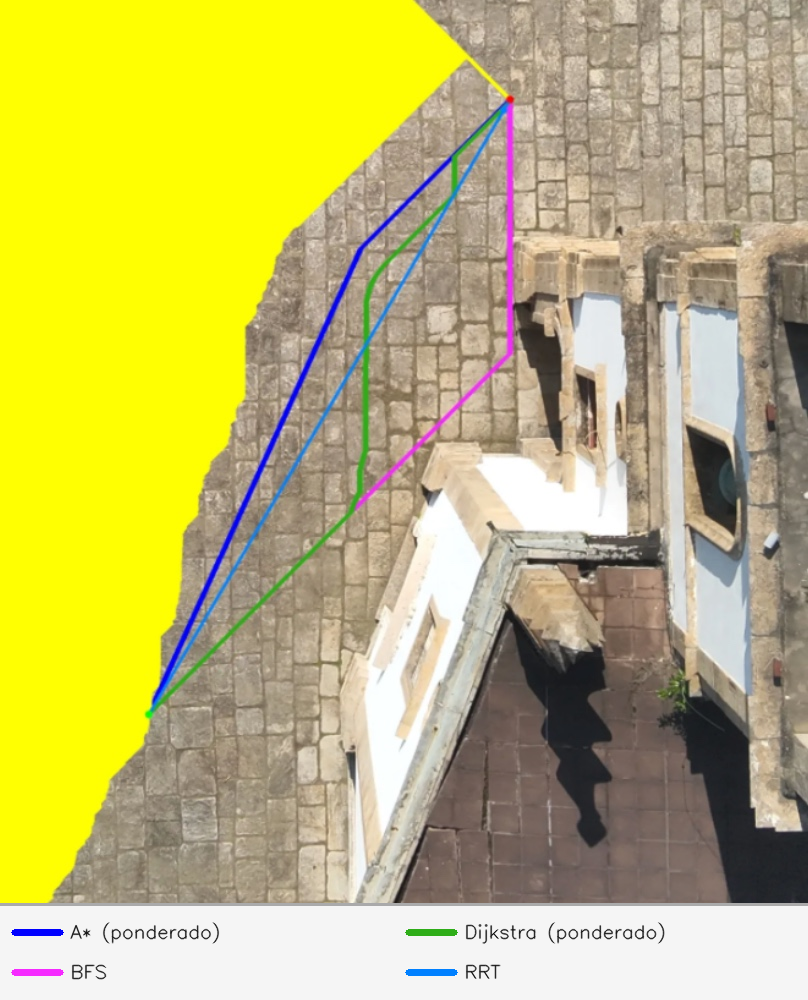
\includegraphics[width=0.66\textwidth]{figuras/caminhos_aerea.png}
    \caption{Detalhe dos caminhos calculados pelos diferentes algoritmos sobre imagem aérea do Outeiro da Glória. Em amarelo, a região classificada como não transitável; marcador vermelho no ponto de partida e verde no de chegada. As cores dos traços seguem a convenção do módulo de pós-processamento, reproduzida na legenda.}
    \label{fig:caminhos_aerea}
\end{figure}

A partir dos caminhos resultantes dos diferentes algoritmos, podemos observar os seguintes pontos. Primeiro, a BFS, em magenta, contorna o obstáculo pelo trajeto com menor número de passos, o que a leva a acompanhar de perto a borda da região não transitável e a fazer uma curva acentuada, sem manter distância de segurança. Segundo, o A* e o Dijkstra, em azul e verde, produzem caminhos distintos apesar de terem o mesmo custo ponderado: em um grafo em grade com pesos idênticos em regiões amplas, há muitos caminhos de custo mínimo, e a ordem de expansão de cada algoritmo determina qual deles é registrado, conforme discutido na Seção~\ref{sec:caminhos_minimos}; ambos estão corretos. Terceiro, o RRT, em azul claro, tem um comportamento diferente: o seu traçado não segue a grade de pixels, sendo formado por poucos segmentos retos que ligam pontos amostrados ao acaso, marcados pelos pequenos círculos ao longo da linha. Nesta cena, quase toda a faixa entre origem e destino é livre, e o viés para o objetivo faz o RRT convergir quase em linha reta com apenas 30 vértices, contra os 879 dos algoritmos de busca.

\subsection{Comparação sobre o Mapa de Ocupação do Mundo Simulado}
\label{subsec:res_warehouse}

A comparação anterior foi repetida sobre o mapa de ocupação do mundo \textit{warehouse}, gerado conforme a Seção~\ref{sec:mapa_ocupacao}. Esse cenário é mais exigente do que a cena aérea aberta: há prateleiras longas e paralelas, corredores estreitos e paredes internas, de modo que o espaço livre entre origem e destino não é um corredor único e amplo. O grafo resultante tem 502.833 vértices e 3.753.214 arestas, a partir de uma imagem de $863 \times 1242$ pixels com resolução de 0,05 m por pixel. O ponto de partida fica no salão central do galpão e o de chegada, junto ao canto superior direito. Cada algoritmo foi executado três vezes, e a coluna de tempo reporta a mediana das três execuções; o RRT foi executado com semente fixa, de modo que as três execuções produziram o mesmo caminho. Os resultados obtidos são apresentados na Tabela~\ref{tab:comparacao_warehouse}, e os caminhos correspondentes, desenhados separadamente para cada algoritmo, na Figura~\ref{fig:caminhos_warehouse}.

\begin{table}[H]
    \centering
    \caption{Comparação dos algoritmos sobre o mapa de ocupação do mundo \textit{warehouse} ($863 \times 1242$ pixels, 502.833 vértices e 3.753.214 arestas; mesmos pontos de início e fim). Valem aqui as mesmas observações da Tabela~\ref{tab:comparacao_algoritmos} quanto às colunas. O tempo é a mediana de três execuções.}
    \label{tab:comparacao_warehouse}
    \small
    \setlength{\tabcolsep}{5pt}
    \begin{tabular}{lrrrrr}
        \toprule
        \textbf{Algoritmo}
            & \shortstack[r]{\textbf{Vértices}\\\textbf{($k+1$)}}
            & \shortstack[r]{\textbf{Custo}\\\textbf{$\ell(P)$}}
            & \shortstack[r]{\textbf{Vért. expl.}\\\textbf{ou iter.}}
            & \shortstack[r]{\textbf{Tempo}\\\textbf{(s)}}
            & \shortstack[r]{\textbf{Distância}\\\textbf{(px)}} \\
        \midrule
        A* (ponderado)       &   609 &  28.714,2 & 391.239 & 2,173 &   709,1 \\
        Dijkstra (ponderado) &   609 &  28.714,2 & 397.659 & 1,694 &   709,1 \\
        BFS                  &   599 &  44.174,4 & 414.703 & 0,674 &   722,3 \\
        DFS                  & 2.614 & 233.982,4 & 467.072 & 0,843 & 3.693,7 \\
        RRT                  &    23 &     758,5 &     230 & 0,073 &   757,3 \\
        \bottomrule
    \end{tabular}
\end{table}

\begin{figure}[H]
    \centering
    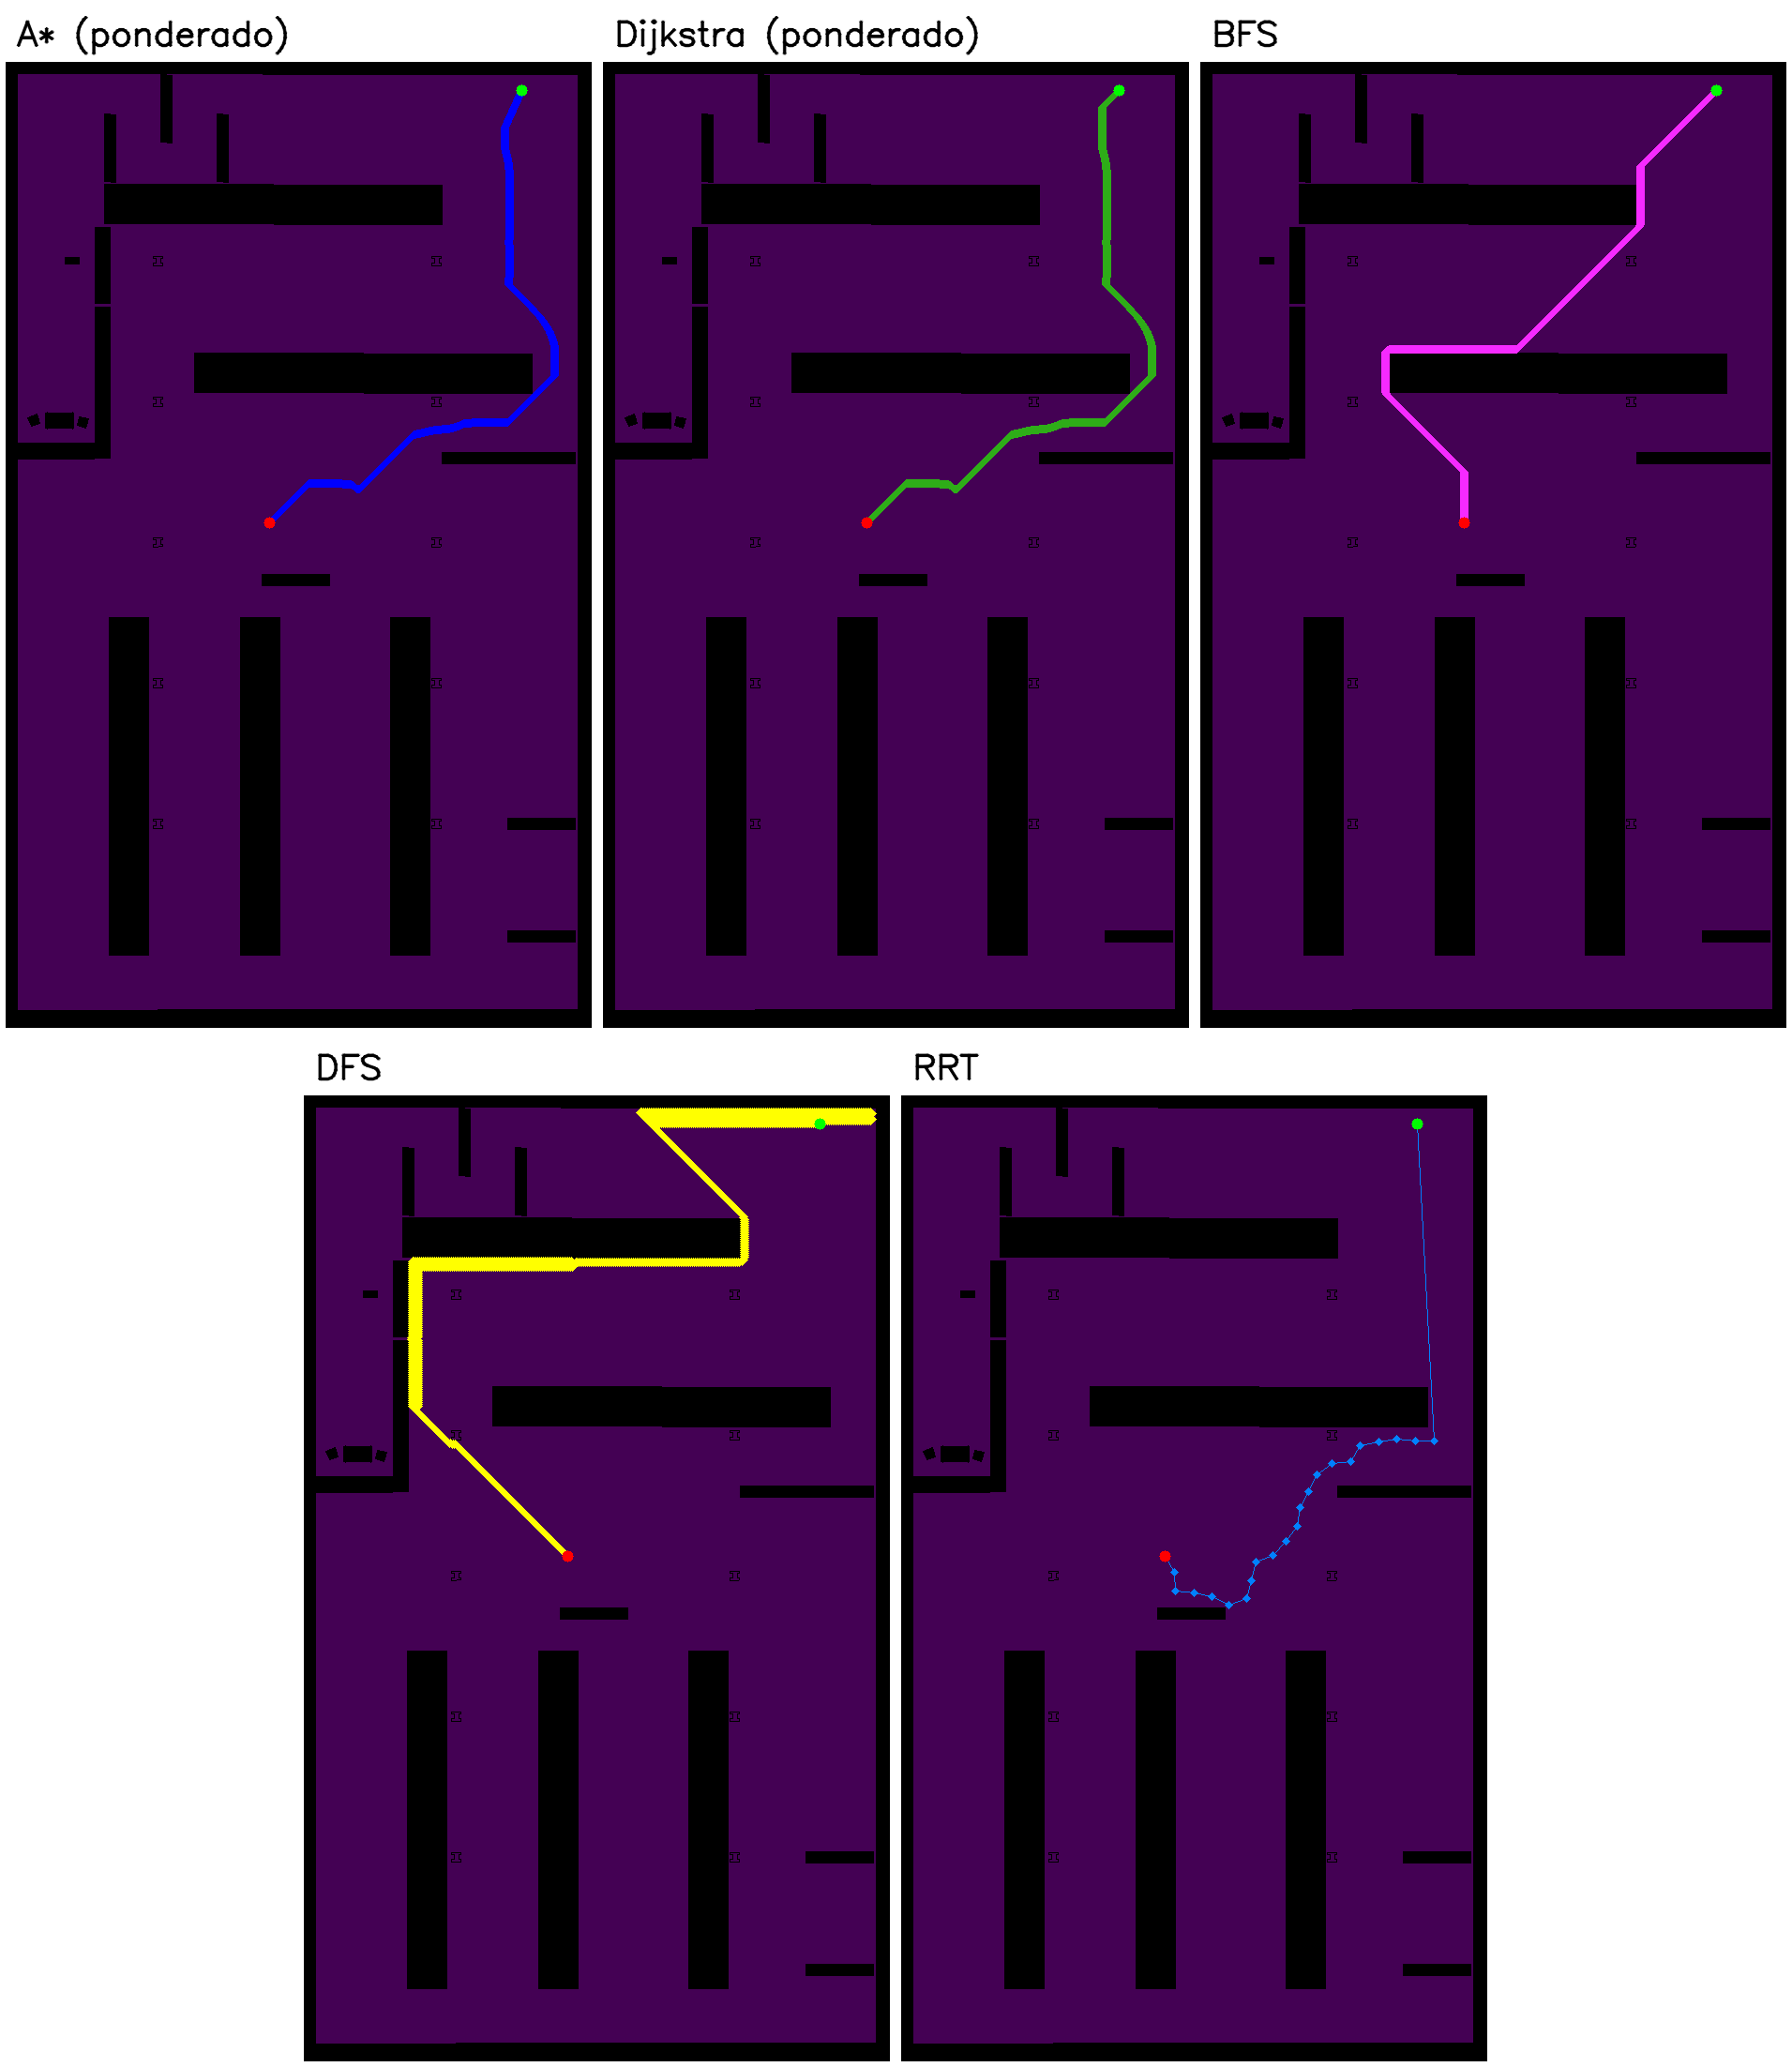
\includegraphics[width=\textwidth]{figuras/caminhos_warehouse_painel.png}
    \caption{Caminhos calculados por cada algoritmo sobre o mapa de ocupação do mundo \textit{warehouse}, desenhados separadamente: A* ponderado (azul), Dijkstra ponderado (verde), BFS (magenta), DFS (amarelo) e RRT (azul claro, com os vértices da árvore marcados por pequenos círculos). Marcador vermelho no ponto de partida e verde no de chegada. A imagem foi recortada na área interna do galpão.}
    \label{fig:caminhos_warehouse}
\end{figure}

Neste cenário, o A* e o Dijkstra devolveram caminhos ligeiramente diferentes, ambos com 609 vértices e exatamente o mesmo custo, $\ell(P^\ast) = 28.714{,}2$, o que ilustra a não unicidade do caminho mínimo discutida na Seção~\ref{sec:caminhos_minimos}. Com a ponderação por proximidade a obstáculos, ambos contornam as prateleiras pelo meio dos corredores. O A* novamente explorou menos vértices que o Dijkstra, ainda que por margem pequena, e novamente levou mais tempo de execução, pelo motivo já discutido. A BFS encontrou um caminho com menos vértices e custo ponderado 54\% maior, seguindo um trajeto completamente distinto, que sobe pelo lado esquerdo da prateleira central e passa rente às suas bordas, por ignorar a penalização por proximidade a obstáculos. A DFS produziu um caminho de 2.614 vértices, com distância cerca de cinco vezes maior que a do A*, formado por longos trechos que acompanham as paredes e as prateleiras até o canto superior esquerdo do galpão, para só então voltar em direção ao destino.

O caminho do RRT é o que mais se diferencia dos demais nesta figura. Com apenas 23 vértices e 230 iterações, ele produziu um caminho com comprimento geométrico próximo ao dos demais, 757,3 px contra 709,1 px, mas com forma visivelmente diferente: enquanto os caminhos determinísticos descrevem curvas suaves e regulares, que acompanham a geometria dos corredores, o traçado do RRT é uma sucessão de segmentos curtos com mudanças bruscas de direção, avançando ora para um lado, ora para o outro, sem relação com a disposição dos obstáculos, seguida de um segmento final longo, quando o último vértice acrescentado passa a ter linha de visada desobstruída até o destino. Esses desvios são consequência direta do mecanismo do algoritmo, descrito na Seção~\ref{sec:rrt}: cada vértice novo é gerado na direção de um ponto amostrado ao acaso, e não na direção do destino, de modo que o caminho reproduz a irregularidade dessa amostragem. A comparação entre as duas figuras mostra que a intensidade desses desvios depende do cenário: na cena aérea aberta da Figura~\ref{fig:caminhos_aerea}, o viés para o objetivo mantém o traçado quase reto; no galpão da Figura~\ref{fig:caminhos_warehouse}, com obstáculos distribuídos ao longo do percurso, o mesmo algoritmo produz desvios pronunciados.

Essa diferença na forma do caminho é importante para um veículo de tração diferencial. Cada mudança brusca de direção obriga o robô a reduzir a velocidade linear e girar, conforme a lei de controle da Seção~\ref{sec:ros_integracao}. Um caminho geometricamente curto, porém com muitos desvios, pode levar mais tempo para ser percorrido do que um caminho um pouco mais longo e suave. Por esse motivo, e apesar do tempo de planejamento muito menor, o RRT não foi adotado como planejador padrão para os ensaios de simulação, nos quais se utilizou o A* ponderado.

% -- 4.3 -------------------------------------------------------------------
\section{Validação no Simulador Gazebo}
\label{sec:res_gazebo}

A integração descrita na Seção~\ref{sec:ros_integracao} foi verificada em execução completa. A partir do \textit{pipeline}, a trajetória planejada é publicada nos tópicos ROS 2 e o UGV Clearpath Jackal simulado no Gazebo a percorre efetivamente, seguindo os \textit{waypoints} por meio do \texttt{path\_\allowbreak{}follower\_\allowbreak{}node} até alcançar o ponto de destino, momento em que o nó registra a conclusão do percurso e publica um comando de velocidade nula, que faz o robô parar.

\subsection{Percursos Executados}

Todos os ensaios foram realizados no mesmo mundo simulado, o \textit{warehouse} (Seção~\ref{sec:mapa_ocupacao}), com o simulador em modo \textit{headless} (Seção~\ref{sec:lim_sim}). Em todos eles, o caminho foi planejado pelo A* ponderado, publicado pela ponte ROS 2 e seguido pelo \texttt{path\_\allowbreak{}follower\_\allowbreak{}node} com velocidade de cruzeiro de 0,4 m/s. Os ensaios diferem apenas na imagem sobre a qual o caminho é planejado. A posição do robô foi registrada a partir da sua odometria (Seção~\ref{sec:odometria}) por um gravador que desenha o rastro do veículo sobre a imagem do caminho planejado. Foram realizados três ensaios, todos concluídos com o robô alcançando o destino:

\begin{enumerate}
    \item \textbf{Percurso de referência em mapa sintético.} O caminho foi planejado pelo A* sobre uma imagem sintética de $400 \times 400$ pixels, gerada para este teste, composta por uma única região quadrada livre, sem obstáculos. Os pontos de partida e de chegada foram escolhidos pelo operador em cantos opostos do quadrado, de modo que o caminho resultante é uma reta diagonal de 281 \textit{waypoints}, correspondente a cerca de 20 m no referencial do mundo, com resolução de 0,05 m por pixel. Como essa imagem não tem relação com a geometria do mundo simulado, o ensaio verifica apenas se o caminho é publicado, seguido pelo robô e se a chegada ao destino é detectada, sem desvio de obstáculos. O registro durou 93,9 s, com 4.601 amostras de odometria, cerca de 49 amostras por segundo. Esse tempo inclui o intervalo entre o início do gravador e a publicação do caminho, porque o gravador precisa ser iniciado antes; por isso, a razão entre a extensão do caminho e a duração do registro, de cerca de 0,21 m/s, subestima a velocidade real do veículo durante o movimento. A Figura~\ref{fig:exp_sintetico} mostra a entrada e a saída do ensaio;
    \item \textbf{Percurso sobre imagem aérea real.} O caminho foi planejado pelo A* sobre a imagem de drone do Outeiro da Glória descrita na Seção~\ref{sec:ambiente}, redimensionada para $800 \times 600$ pixels e segmentada pela U-Net com \textit{backbone} MobileNet V2. O percurso liga um ponto na rua estreita, no alto da imagem, a um ponto no pátio pavimentado, embaixo, contornando as edificações e os veículos estacionados. Também aqui a imagem não corresponde à geometria do mundo simulado: o ensaio avalia o seguimento, pelo veículo, de um caminho planejado sobre uma imagem aérea real, e não o desvio dos obstáculos do mundo. O registro durou 232,9 s, tempo que inclui o deslocamento inicial do robô desde a posição em que foi criado até o primeiro \textit{waypoint}, discutido na Seção~\ref{subsec:alinhamento}. A Figura~\ref{fig:exp_dji} mostra a entrada, com o caminho do A*, e a saída do ensaio;
    \item \textbf{Percurso no mundo \textit{warehouse} com o mapa de ocupação do próprio mundo.} O caminho foi planejado pelo A* sobre o mapa de ocupação da Seção~\ref{sec:mapa_ocupacao}, com os mesmos pontos de partida e de chegada da Tabela~\ref{tab:comparacao_warehouse}, mas com folga mínima maior, de 12 pixels (0,6 m), para garantir margem de segurança em relação às dimensões do Jackal. Este é o único dos três ensaios em que o mapa corresponde exatamente ao mundo em que o robô se move, de modo que o caminho desvia dos obstáculos reais do galpão. O caminho publicado tem 621 \textit{waypoints} e 35,8 m. Com o robô reposicionado no primeiro \textit{waypoint} antes do início (Seção~\ref{subsec:alinhamento}) e o início do movimento identificado nos registros de odometria, o veículo percorreu 35,1 m em 95,8 s, com velocidade média de 0,37 m/s, próxima à de cruzeiro, e 4.537 amostras de odometria, cerca de 47 por segundo. A Figura~\ref{fig:exp_warehouse} mostra a entrada e a saída do ensaio.
\end{enumerate}

\begin{figure}[H]
    \centering
    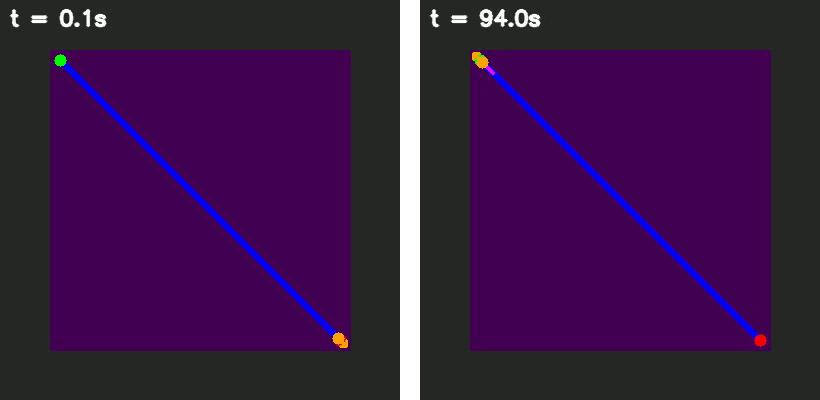
\includegraphics[width=0.75\textwidth]{figuras/exp_sintetico.png}
    \caption{Percurso de referência em mapa sintético. (a) Entrada: caminho planejado pelo A* (azul) sobre a imagem sintética, com o UGV (laranja) no ponto de partida. (b) Saída: fim do percurso, com o UGV sobre o ponto de chegada.}
    \label{fig:exp_sintetico}
\end{figure}

\begin{figure}[H]
    \centering
    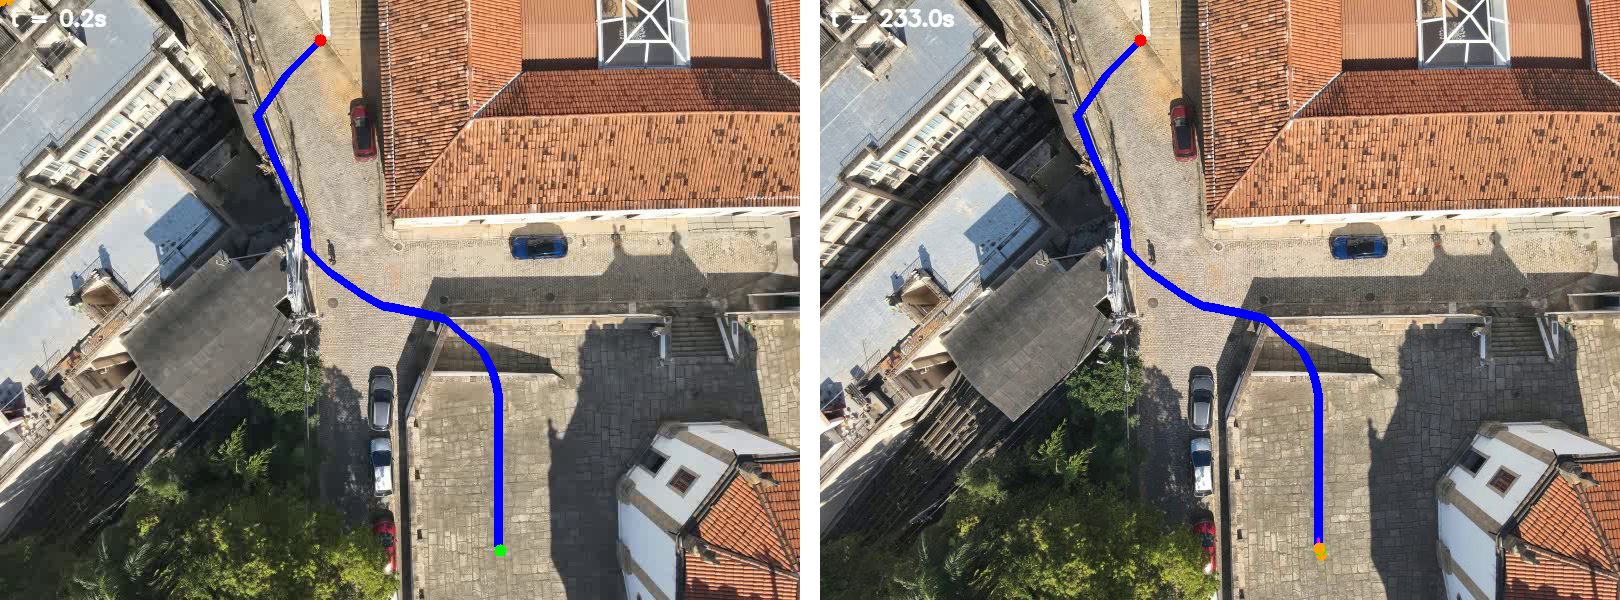
\includegraphics[width=\textwidth]{figuras/exp_dji.png}
    \caption{Percurso sobre imagem aérea real do Outeiro da Glória. (a) Entrada: caminho planejado pelo A* (azul), único caminho publicado para o robô, com o ponto de partida em vermelho e o de chegada em verde. (b) Saída: fim do percurso ($t = 233{,}1$ s), com o UGV simulado (laranja) sobre o ponto de chegada e o rastro recente da odometria em magenta.}
    \label{fig:exp_dji}
\end{figure}

\begin{figure}[H]
    \centering
    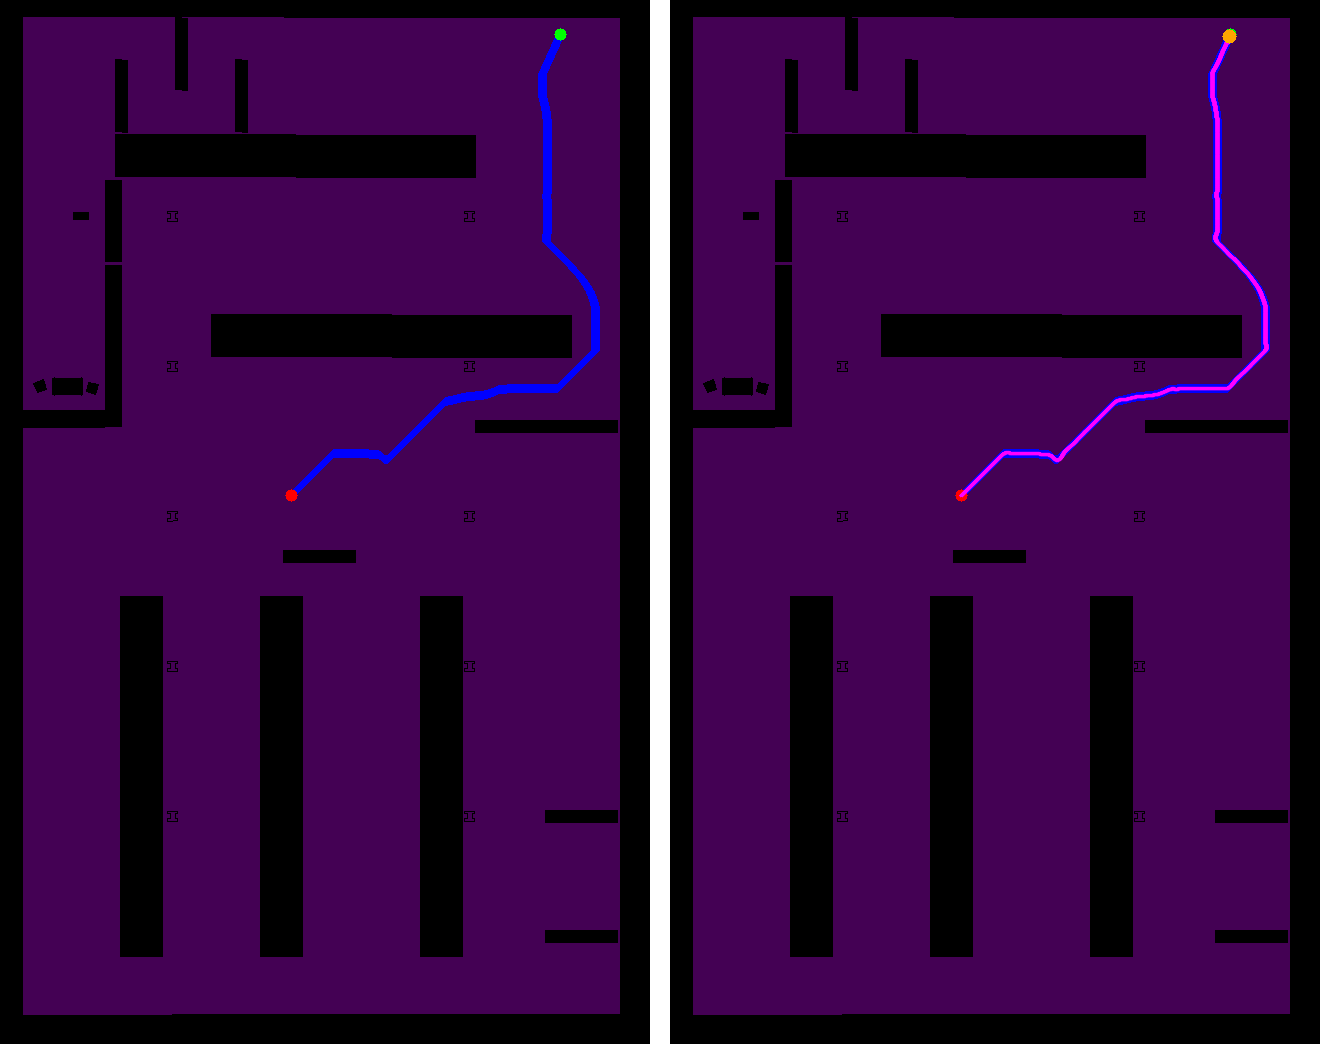
\includegraphics[width=0.9\textwidth]{figuras/exp_warehouse.png}
    \caption{Percurso no mundo \textit{warehouse}, planejado sobre o mapa de ocupação do próprio mundo. (a) Entrada: caminho planejado pelo A* (azul), do ponto de partida (vermelho) ao de chegada (verde). (b) Saída: rastro completo da odometria do UGV simulado (magenta), sobreposto ao caminho planejado, com a posição final do veículo em laranja.}
    \label{fig:exp_warehouse}
\end{figure}

\subsection{Aderência entre a Trajetória Planejada e a Executada}

A sobreposição do rastro de odometria ao caminho planejado, visível nas Figuras~\ref{fig:exp_dji} e \ref{fig:exp_warehouse}, mostra que o veículo segue o traçado planejado ao longo de todo o percurso. Os desvios observados concentram-se nas mudanças de direção, onde o veículo descreve uma curva de raio finito enquanto o caminho planejado tem um vértice.

Para o percurso no mundo \textit{warehouse}, o gravador passou a salvar, além do vídeo, as amostras de odometria e o caminho publicado, ambos no referencial do mundo, o que permitiu calcular o erro lateral: para cada amostra de posição, a menor distância até o caminho planejado, tratado como uma poligonal. O erro lateral médio foi de 0,8 cm, com raiz do erro quadrático médio de 1,3 cm, 95\% das amostras abaixo de 2,9 cm e máximo de 7,1 cm. Esses valores são inferiores à tolerância de \textit{waypoint} configurada, de 0,12 m. O robô parou a 0,15 m do ponto de chegada, valor que coincide com a tolerância de chegada configurada no seguidor.

Essa medida tem uma limitação: o erro foi calculado em relação à odometria, que é a mesma estimativa de posição usada pelo seguidor para se controlar. Ele mede, portanto, a qualidade do seguimento do caminho, e não o erro de localização absoluta do veículo, que, em um robô real, incluiria também a deriva da odometria (Seção~\ref{sec:odometria}). Para os dois primeiros ensaios, os dados brutos de odometria não foram salvos, e a avaliação é apenas visual.

\subsection{Alinhamento entre Referenciais}
\label{subsec:alinhamento}

O fator que mais influenciou os resultados da simulação foi a correspondência entre o referencial da imagem e o do mundo, discutida na Seção~\ref{sec:gsd}. O veículo é criado no mundo simulado na origem, ao passo que o caminho planejado começa no pixel escolhido pelo operador, que corresponde a outro ponto do mundo. Sem correção, o seguidor interpreta o primeiro \textit{waypoint} como um destino a alcançar e o robô dirige-se até lá antes de iniciar o percurso propriamente dito. Quando a origem informada está errada, esse trecho inicial pode sair inteiramente da área representada pelo mapa, e o percurso registrado parece extrapolar os limites do ambiente.

Duas soluções foram implementadas e verificadas. A primeira é informar corretamente a origem em metros, o que o conversor de mundos da Seção~\ref{sec:mapa_ocupacao} passou a calcular automaticamente para o caso do Gazebo. A segunda é reposicionar o veículo no primeiro \textit{waypoint} antes do início do percurso, recurso disponível por parâmetro no seguidor, com a devida composição da transformação entre os referenciais de odometria e de mundo, para que a estimativa de pose permaneça coerente após o reposicionamento. A primeira solução é a correta para uso realista; a segunda é útil para isolar a avaliação do seguidor da questão de alinhamento.

Em resumo, o simulador recebe como entrada o modelo do robô e do mundo, com geometria, dinâmica e sensores, e os comandos de velocidade gerados pelo seguidor; como saída, publica o estado simulado do veículo, em especial a odometria e as transformações de referencial, além dos fluxos de sensores. Essa odometria é usada pelo \texttt{path\_\allowbreak{}follower\_\allowbreak{}node} para calcular os novos comandos, o que forma a malha de controle em ciclo fechado.

% -- 4.4 -------------------------------------------------------------------
\section{Limitações e Dificuldades Encontradas}
\label{sec:limitacoes}

Esta seção reúne as limitações do trabalho e as dificuldades que determinaram o seu estágio final, em particular a não realização dos ensaios em ambiente real.

\subsection{Ausência de Validação em Ambiente Real}

O planejamento inicial do projeto previa, para os dois últimos meses, a repetição dos ensaios de simulação em um veículo físico. Essa etapa não foi realizada. As razões são de três naturezas.

A primeira é de \textbf{disponibilidade de plataforma}. Os ensaios de simulação foram conduzidos sobre o modelo do Clearpath Jackal, escolhido por ser uma plataforma de tração diferencial com modelo bem mantido e integração madura com o ROS 2. A transposição para um veículo físico exigiria um UGV com odometria confiável, unidade inercial e interface ROS 2 disponível para uso continuado durante o período de ensaios, condição que não foi possível assegurar dentro do prazo do projeto.

A segunda é de \textbf{espaço e de aquisição de imagem}. O método proposto depende de uma imagem aérea da mesma área em que o veículo vai operar, capturada com a câmera próxima da vertical e com escala conhecida. Isso significa que um ensaio real não se restringe a posicionar o robô em um corredor: é necessário um espaço aberto, com obstáculos permanentes e área livre suficiente para percursos de algumas dezenas de metros, e um voo de UAV sobre esse espaço, com autorização, condições meteorológicas adequadas e medição de referência para determinação do fator de escala em metros por pixel. A coordenação dessas condições, somada à necessidade de repetir o voo caso a imagem não ficasse adequada, tornou o ensaio real incompatível com o prazo remanescente.

A terceira é de \textbf{tempo}. A integração com o ROS 2 e a simulação, prevista para ser uma etapa intermediária, consumiu parcela significativa do prazo do projeto. A depuração da comunicação entre os nós, o tratamento das políticas de QoS, a configuração do \textit{workspace} do simulador e, principalmente, os problemas de ambiente gráfico descritos a seguir ocuparam o período que estava reservado para a transição ao ambiente real.

É importante delimitar o que essa ausência deixa de fora. Todo o encadeamento entre o planejamento e o controle do veículo, isto é, a publicação do caminho, o seguimento de \textit{waypoints}, a realimentação por odometria e a detecção de chegada ao destino, foi verificado em ciclo fechado e usa exatamente as mesmas interfaces que seriam usadas com um robô físico. O que não foi verificado são os aspectos que só o mundo real apresenta: irregularidade e escorregamento do terreno, deriva da odometria acumulada ao longo de percursos longos, erros de georreferenciamento da imagem aérea e obstáculos não presentes no momento da captura da imagem.

\subsection{Limitações do Ambiente de Simulação}
\label{sec:lim_sim}

A simulação foi executada em ROS 2 Humble e Gazebo sobre Ubuntu 22.04 em WSL2. Nessa configuração, a interface gráfica tridimensional do Gazebo não pôde ser utilizada de forma confiável. A tentativa de abrir o cliente gráfico resultava em falha do motor de renderização, e a alternativa de renderização por \textit{software} produzia, na maior parte das tentativas, janela preta ou travada. Apenas em algumas sessões abertas manualmente, de forma interativa, a interface com renderização por \textit{software} chegou a funcionar, o que permitiu inspecionar o mundo e obter a Figura~\ref{fig:gazebo_jackal}; esse modo, porém, não se mostrou reprodutível nem estável o suficiente para acompanhar os ensaios de percurso. A investigação identificou que o compositor gráfico do WSL2 opera inteiramente em \textit{software}, sem aceleração, por limitação do suporte a gerenciamento de memória gráfica no driver utilizado, o que não é contornável pela atualização do subsistema nem dos pacotes gráficos da distribuição.

A solução adotada foi executar o simulador em modo \textit{headless}, sem interface gráfica, que se mostrou inteiramente confiável, e registrar os percursos por um gravador que recebe a odometria do veículo e desenha, em vídeo bidimensional, a posição do robô e o seu rastro sobre a imagem do caminho planejado. As figuras de execução deste capítulo são quadros desses vídeos ou, no caso da Figura~\ref{fig:exp_warehouse}(b), o rastro completo desenhado a partir das amostras de odometria registradas. Essa limitação afetou apenas a inspeção visual da simulação, e não a simulação em si: a dinâmica, os sensores e o controle foram calculados normalmente pelo servidor do simulador.

\subsection{Outras Limitações}

\begin{itemize}
    \item \textbf{Generalização da segmentação.} Os modelos utilizados foram treinados sobre o \emph{Semantic Drone Dataset}, cujas imagens têm características de altitude, ângulo e tipo de cenário distintas das imagens usadas nos ensaios. Em particular, o conjunto de treinamento cobre altitudes de 5 a 30 m (Seção~\ref{sec:sdd}), enquanto a imagem do percurso simulado foi capturada a cerca de 41 m, o que torna os objetos menores na imagem do que nos exemplos de treinamento. A qualidade da máscara em cenários muito diferentes dos de treinamento não foi quantificada, porque as imagens de ensaio não são anotadas. A avaliação aqui apresentada é, portanto, a métrica divulgada sobre as imagens de teste do conjunto original acompanhada de inspeção visual sobre as imagens deste trabalho;
    \item \textbf{Planejamento estático.} O sistema resolve o planejamento global sobre um mapa fixo. Obstáculos que apareçam, desapareçam ou se movam durante a execução não são tratados, e o caminho não é replanejado;
    \item \textbf{Entrega repetida do caminho.} Nos ensaios, apenas a primeira mensagem de caminho recebida por um nó seguidor recém-iniciado foi processada de forma consistente. Publicações subsequentes, com o seguidor já em execução há algum tempo, nem sempre foram entregues. O procedimento adotado foi reiniciar o nó seguidor antes de cada nova publicação. O problema ocorreu inclusive no percurso do mundo \textit{warehouse}: nas três primeiras publicações o caminho chegou ao gravador, mas não ao seguidor, e foi necessário reiniciar o seguidor e publicar novamente. A causa provável está na combinação entre a política de durabilidade e a duração curta do processo que publica, e a correção fica registrada como pendência;
    \item \textbf{Escala do grafo.} A matriz de adjacência já é mantida no formato esparso \textit{Compressed Sparse Row} \cite{saad2003}, mas a lista de arestas e os seus atributos (pesos e comprimentos) são armazenados explicitamente, um registro por aresta, com cerca de oito arestas por vértice. Para as imagens utilizadas, de até cerca de $10^6$ pixels, isso é viável, mas o consumo de memória cresce de forma proporcional ao número de arestas e passa a ser limitante para imagens de resolução maior;
    \item \textbf{Variabilidade do RRT.} Todos os valores reportados para o RRT correspondem a execuções com uma única semente fixa do gerador de números pseudoaleatórios. Uma caracterização estatística adequada exigiria repetir cada cenário muitas vezes e reportar média e dispersão, o que não foi feito.
\end{itemize}

% ======================================================================
\chapter{CONCLUSÃO}
\label{cap:conclusao}
% ======================================================================

Este Projeto de Final de Curso partiu do trabalho desenvolvido em 2025 por Almeida e Barbosa \cite{camelo2025}, que havia demonstrado a viabilidade do planejamento de trajetórias por otimização em grafos sobre imagens aéreas previamente segmentadas, e o levou até a execução efetiva do caminho por um veículo, ainda que em ambiente simulado.

A base do trabalho é uma arquitetura modular e orientada a objetos, com cinco estágios encadeados e interfaces abstratas, sobre a qual foram reimplementados os algoritmos BFS, DFS, Dijkstra e A* com uma representação genérica de grafo. A principal vantagem dessa arquitetura é a facilidade de extensão: novos algoritmos de planejamento ou modelos de segmentação podem ser incluídos sem alterar os demais módulos do sistema.

Sobre essa estrutura, o algoritmo RRT foi acrescentado ao catálogo, permitindo comparar diretamente o planejamento por amostragem com a busca em grafos sobre os mesmos mapas. A segmentação semântica, técnica de aprendizado de máquina, deixou de ser uma dependência externa e passou a ser executada dentro do \textit{pipeline}, com modelos U-Net pré-treinados \cite{junior2024_models}, o que permitiu partir de imagens RGB reais de drone em vez de mapas já segmentados. E o pós-processamento foi ligado ao ROS 2 e ao Gazebo, de modo que o caminho calculado passou a ser percorrido por um UGV simulado.

Por fim, foi tratada a correspondência métrica entre o mapa em que o caminho é planejado e o mundo em que o robô se move. A conversão automática da descrição do mundo simulado em mapa de ocupação eliminou o ajuste manual do fator de escala e da origem, e separou os erros de planejamento dos erros de alinhamento de referenciais. Com isso, os ensaios em ambiente virtual foram concluídos: o veículo simulado percorre integralmente as trajetórias planejadas, em três cenários distintos, chegando ao destino em todos eles. No percurso sobre o mapa do próprio mundo simulado, o erro lateral médio entre a trajetória executada e a planejada foi inferior a 1 cm.

Quanto aos algoritmos, os resultados reproduzem e detalham as conclusões do PFC 2025. O A* e o Dijkstra devolvem soluções de mesmo custo, com o A* explorando menos vértices; o ganho em vértices explorados, entretanto, não se traduziu automaticamente em ganho de tempo nos grafos densos deste trabalho, o que mostra que a escolha entre os dois depende do tamanho do problema. A BFS produz o caminho geometricamente mais curto e o mais arriscado, por ignorar a penalização de proximidade. A DFS confirma-se inadequada ao problema. O RRT é muito mais rápido no cálculo do caminho: o seu tempo de planejamento foi de 9 a 43 vezes menor que o dos algoritmos de busca nos dois cenários avaliados (Tabelas~\ref{tab:comparacao_algoritmos} e \ref{tab:comparacao_warehouse}). Em compensação, produz caminhos irregulares, com desvios que variam entre execuções e que se acentuam em ambientes com obstáculos distribuídos, o que o torna menos adequado para um veículo de tração diferencial, que precisa reduzir a velocidade a cada mudança brusca de direção.

Em resumo, o sistema está completo e foi verificado, em ambiente simulado, desde a imagem aérea até o movimento do veículo. Como trabalho futuro é proposta a validação em ambiente real, que, embora prevista no planejamento inicial, não foi realizada por restrições de disponibilidade de plataforma física, de espaço adequado para ensaio com captura aérea associada e de tempo remanescente, conforme detalhado na Seção~\ref{sec:limitacoes}. Como todas as interfaces entre o planejamento e o veículo são as mesmas que seriam usadas com um robô físico, essa transição não exige mudanças no \textit{software}; o que faltou foram a plataforma física e o tempo necessário para os ensaios.

% -- 5.1 -------------------------------------------------------------------
\section{Perspectivas Futuras}
\label{sec:perspectivas}

As continuidades identificadas, em ordem aproximada de prioridade, são:

\begin{enumerate}
    \item \textbf{Validação em ambiente real.} Repetir os ensaios de simulação em um UGV físico, sobre imagem aérea da própria área de ensaio, com fator de escala determinado por referência medida em campo. Somente essa etapa permite avaliar os efeitos de terreno irregular, escorregamento e deriva da odometria;
    \item \textbf{Métrica quantitativa de aderência para todos os planejadores.} Estender o cálculo do erro lateral, feito aqui para um percurso do A*, a percursos executados a partir dos caminhos de todos os algoritmos, e usá-lo para comparar objetivamente esses caminhos quanto à facilidade de execução, e não apenas quanto ao custo de planejamento;
    \item \textbf{Ambientes dinâmicos.} Estender o sistema para tratar obstáculos que aparecem, desaparecem ou se movem durante a execução, o que exige replanejamento em tempo real. Para esse caso, o RRT e as suas variantes voltadas a ambientes dinâmicos \cite{xu2024} são candidatos naturais, pelo baixo tempo de planejamento e por dispensarem a reconstrução do grafo a cada mudança (Seção~\ref{sec:rrt}), assim como algoritmos de replanejamento incremental sobre grafos. Essa era, aliás, a primeira perspectiva futura apontada pelo PFC 2025 e permanece em aberto;
    \item \textbf{Seleção automática e alternância entre algoritmos.} Os resultados do Capítulo~\ref{cap:resultados} mostram que nenhum planejador é o melhor em todos os cenários: o A* e o Dijkstra devolvem os caminhos de menor custo, o RRT planeja de 9 a 43 vezes mais rápido, mas produz caminhos irregulares e tem dificuldade em passagens estreitas, e a vantagem do A* sobre o Dijkstra em tempo depende do tamanho do grafo. Isso motiva um processo decisório que escolha o algoritmo a partir das características da imagem fornecida ao sistema, problema conhecido na literatura como seleção de algoritmos \cite{rice1976, kerschke2019}. Características simples de extrair do mapa de navegabilidade e do grafo, como a fração de área transitável, o número de vértices, a largura dos corredores livres (obtida da transformada de distância já calculada na construção do grafo), o número de regiões conexas e a distância entre a origem e o destino, podem alimentar inicialmente regras fixas e, havendo dados suficientes, um classificador treinado sobre execuções anteriores, que indique o algoritmo com o melhor compromisso entre tempo de planejamento e qualidade do caminho. A mesma ideia pode ser levada para dentro de uma única trajetória. O mapa seria dividido em regiões, e cada trecho seria planejado pelo algoritmo mais adequado à região que atravessa: por exemplo, o RRT em áreas abertas, onde encontra um caminho rapidamente, e o A* em corredores estreitos, onde a busca em grafo é mais confiável. Alternativamente, o RRT forneceria um caminho inicial em poucos instantes, para que o veículo comece a se mover, enquanto o A* calcula a solução de menor custo, que substitui a anterior quando estiver pronta. Durante a execução, a alternância se aplica também ao replanejamento: diante de uma mudança no ambiente, recorre-se a um planejador rápido para o desvio local e mantém-se a busca em grafo para o percurso global. Na arquitetura atual, esse seletor pode ser implementado como um novo algoritmo registrado na fábrica, sob a mesma interface \texttt{PathAlgorithm}, que delega o cálculo aos demais planejadores, sem alteração nos outros módulos;
    \item \textbf{Planejamento a partir de nuvens de pontos.} A imagem aérea fornece apenas a projeção bidimensional do terreno: ela não distingue, por exemplo, um gramado plano de um talude de mesma cor, nem informa a altura da vegetação, de meios-fios e de degraus. Nuvens de pontos tridimensionais, obtidas por LiDAR embarcado no UAV ou no próprio UGV, ou por fotogrametria a partir de várias imagens aéreas sobrepostas, permitem estimar a elevação, a declividade e a rugosidade de cada região. Uma forma de aproveitar o \textit{pipeline} existente é projetar a nuvem em uma grade de elevação \cite{fankhauser2016}, na qual cada célula guarda a altura do terreno, e derivar dela tanto a transitabilidade, tornando obstáculos as células com declividade ou degrau acima do suportado pelo veículo, quanto novos termos na função de peso das arestas, como a inclinação a vencer entre vértices vizinhos. Bibliotecas como a \textit{Point Cloud Library} \cite{rusu2011} oferecem a filtragem da nuvem, a separação do plano do solo e a estimação de normais necessárias a esse processamento. A arquitetura já prevê esse tipo de entrada: o módulo \texttt{data\_\allowbreak{}ingestion} define a interface \texttt{PointCloudIngestedData} e a entidade \texttt{PointCloudData}, com as coordenadas, as normais, as cores e a intensidade de cada ponto, de modo que resta implementar um \textit{parser} de grafos para nuvens de pontos e registrá-lo na fábrica correspondente. A nuvem de pontos também pode ser combinada à imagem: a segmentação semântica identifica o tipo de terreno, e a geometria tridimensional corrige os casos em que a cor induz a erro, como sombras e superfícies de cor semelhante ao piso. A escolha entre planejar sobre a imagem, sobre a nuvem ou sobre ambas pode, por sua vez, fazer parte do processo decisório descrito no item anterior;
    \item \textbf{Caracterização estatística do RRT.} Repetir os cenários com diferentes sementes do gerador de números pseudoaleatórios e reportar média e dispersão do comprimento, do tempo e do número de mudanças de direção, de modo a comparar o planejador estocástico com os determinísticos em condições equivalentes;
    \item \textbf{Suavização de trajetória.} Introduzir uma etapa de pós-processamento que substitua vértices agudos por curvas compatíveis com a cinemática do veículo, o que beneficiaria especialmente os caminhos produzidos pelo RRT e pela BFS;
    \item \textbf{Redução do uso de memória do grafo.} Gerar as arestas e os seus pesos sob demanda, durante a busca, a partir das penalidades dos vértices, em vez de armazená-los explicitamente, para viabilizar imagens de resolução maior sem crescimento proporcional do uso de memória.
\end{enumerate}

% ======================================================================
\chapter*{DECLARAÇÃO SOBRE O USO DE INTELIGÊNCIA ARTIFICIAL GENERATIVA}
\addcontentsline{toc}{chapter}{DECLARAÇÃO SOBRE O USO DE INTELIGÊNCIA ARTIFICIAL GENERATIVA}
% ======================================================================

Em conformidade com as recomendações adotadas por periódicos e conferências internacionais para a declaração do uso de tecnologias de inteligência artificial generativa em trabalhos acadêmicos \cite{cope2023, elsevier2024}, os autores declaram o seguinte.

Durante a preparação deste trabalho, foram utilizadas as seguintes ferramentas de inteligência artificial generativa baseadas em grandes modelos de linguagem: o assistente Claude, da empresa Anthropic, inclusive por meio da ferramenta de linha de comando Claude Code, e o GitHub Copilot, assistente de programação integrado ao editor de código. Essas ferramentas foram utilizadas com as seguintes finalidades:

\begin{itemize}
    \item \textbf{Apoio à redação.} Revisão de clareza, coesão, ortografia e uniformidade terminológica do texto, bem como sugestões de organização de seções. Nenhum trecho foi incorporado sem leitura, verificação e edição pelos autores;
    \item \textbf{Apoio ao desenvolvimento de \textit{software}.} Sugestão e revisão de trechos de código, identificação de erros de execução e apoio na configuração do ambiente de simulação. Todo o código foi executado, testado e validado pelos autores, e os resultados apresentados neste trabalho decorrem dessas execuções;
    \item \textbf{Apoio à formatação.} Elaboração e ajuste de estruturas de composição do documento em \LaTeX, incluindo tabelas e diagramas.
\end{itemize}

As ferramentas de inteligência artificial generativa \textbf{não} foram utilizadas para gerar dados experimentais, resultados, medições, figuras de resultados ou referências bibliográficas. Todos os dados e resultados apresentados no Capítulo~\ref{cap:resultados} provêm da execução do sistema descrito no Capítulo~\ref{cap:metodologia} ou de fontes explicitamente citadas. Todas as referências foram verificadas pelos autores quanto à existência e à pertinência.

Nenhuma ferramenta de inteligência artificial figura como autora ou coautora deste trabalho, uma vez que a autoria pressupõe responsabilidade pelo conteúdo, o que não se aplica a tais ferramentas. Após o uso das ferramentas, os autores revisaram e editaram o conteúdo conforme necessário e assumem integral responsabilidade pelo conteúdo deste Projeto de Final de Curso.

Esta declaração refere-se exclusivamente ao uso de inteligência artificial como apoio ao processo de escrita e de desenvolvimento. O emprego de redes neurais para segmentação semântica de imagens, descrito nas Seções~\ref{sec:segmentacao} e \ref{sec:impl_segmentacao}, constitui objeto de estudo e parte do método deste trabalho, está documentado nas seções correspondentes e não se enquadra no escopo desta declaração.

% ==========================================================================
%  REFERENCIAS
% ==========================================================================
\bibliography{referencias_vf_apos_apresentacao}

% ==========================================================================
%  APENDICES
% ==========================================================================
\begin{apendicesenv}

\partapendices

% ----------------------------------------------------------------------
\chapter{GUIA DE INSTALAÇÃO E CONTINUIDADE}
\label{ap:instalacao}
% ----------------------------------------------------------------------
\sloppy
\urlstyle{tt}

Este apêndice reúne as instruções necessárias para que outros grupos instalem o sistema, reproduzam os experimentos e deem continuidade ao trabalho. Todo o código está disponível no repositório \url{https://github.com/tassandro/path_plannig_pfc}. O guia é dividido em duas partes independentes: o \textit{pipeline} de planejamento, que roda em qualquer sistema operacional com Python, e o ambiente de simulação, que exige Linux com ROS 2. Quem pretende trabalhar apenas com segmentação, grafos ou algoritmos precisa somente da primeira parte.

Os comandos foram verificados na configuração descrita na Seção~\ref{sec:ambiente}: Windows 11 com Ubuntu 22.04 em WSL2 e ROS 2 Humble. Uma instalação nativa do Ubuntu 22.04 também atende e é preferível para a simulação, por não sofrer das limitações de interface gráfica descritas na Seção~\ref{sec:lim_sim}.

% -- A.1 ------------------------------------------------------------------
\section{Organização do Repositório}

A Tabela~\ref{tab:repositorio} descreve o conteúdo de cada diretório. Os cinco primeiros correspondem aos módulos da arquitetura apresentada na Seção~\ref{sec:arquitetura}, e cada um segue a mesma organização interna: \texttt{interfaces.py} (classes abstratas), \texttt{entities.py} (\textit{dataclasses}), \texttt{index.py} (fábrica de registro) e \texttt{\_\_init\_\_.py} (exportações públicas).

\begin{table}[htbp]
    \centering
    \caption{Organização do repositório.}
    \label{tab:repositorio}
    \footnotesize
    \renewcommand{\arraystretch}{1.2}
    \begin{tabular}{>{\raggedright\arraybackslash}p{5.1cm} >{\raggedright\arraybackslash}p{9.7cm}}
        \toprule
        \textbf{Caminho} & \textbf{Conteúdo} \\
        \midrule
        \texttt{data\_ingestion/} & Entidades de entrada: imagens (\texttt{ImageData}) e nuvens de pontos (\texttt{PointCloudData}) \\
        \texttt{preprocessing/} & Segmentação semântica (modelos U-Net de \cite{junior2024_models}, prefixo \texttt{drone\_}), limiarização HSV e modelos alternativos \\
        \texttt{graph\_parsing/} & Conversão do mapa em grafo e função de peso (\texttt{\_grid\_utils.py}) \\
        \texttt{algorithm/} & BFS, DFS, Dijkstra, A* e RRT, sob a interface \texttt{PathAlgorithm} \\
        \texttt{post\_processing/} & Geração de \textit{waypoints} e desenho dos caminhos sobre a imagem \\
        \texttt{ros\_bridge/} & Publicação da imagem e do caminho em tópicos ROS 2 (opcional) \\
        \texttt{ros2\_ws/\allowbreak{}src/\allowbreak{}ugv\_bridge/} & Pacote ROS 2 do lado do robô: \texttt{path\_follower\_node}, \texttt{tf\_odom\_bridge\_node}, \texttt{image\_monitor\_node} e \textit{launch files} \\
        \texttt{ros2\_ws/\allowbreak{}JACKAL\_SIMULATION\_GUIDE.md} & Guia detalhado da simulação, com o histórico dos problemas encontrados \\
        \texttt{scripts/} & \texttt{download\_drone\_models.py} (baixa os modelos de segmentação) e \texttt{gazebo\_world\_to\_occupancy.py} (gera o mapa de ocupação de um mundo do Gazebo) \\
        \texttt{main.py} & Interface de linha de comando do \textit{pipeline} \\
        \texttt{gui.py} & Interface gráfica de teste, executada no navegador \\
        \texttt{models/}, \texttt{data/}, \texttt{output/} & Modelos, imagens de entrada e resultados; não versionados \\
        \bottomrule
    \end{tabular}
\end{table}

Os diretórios \texttt{models/} e \texttt{data/} estão no \texttt{.gitignore} por causa do tamanho dos arquivos. Os modelos são baixados pelo \textit{script} descrito na Seção~\ref{sec:ap_pipeline}. As imagens aéreas usadas nos ensaios, do Outeiro da Glória, não estão no repositório e devem ser solicitadas aos orientadores; qualquer imagem RGB nadiral pode ser usada em seu lugar.

% -- A.2 ------------------------------------------------------------------
\section{Requisitos}

\begin{itemize}
    \item \textbf{Somente planejamento:} Python 3.10 ou superior, em Windows, Linux ou macOS. A segmentação usa a GPU automaticamente quando há suporte a CUDA (NVIDIA) ou MPS (Apple Silicon) e, caso contrário, roda na CPU, mais lentamente. Os cinco modelos de segmentação ocupam, juntos, algumas centenas de megabytes;
    \item \textbf{Simulação:} Ubuntu 22.04 (nativo ou em WSL2), ROS 2 Humble, Gazebo (instalado com o pacote \texttt{ros-humble-ros-gz}), o simulador da Clearpath (\texttt{clearpath\_\allowbreak{}simulator}, ramo \texttt{humble}) e as ferramentas \texttt{colcon}, \texttt{rosdep} e \texttt{vcstool}. Recomenda-se ao menos 16 GB de memória.
\end{itemize}

% -- A.3 ------------------------------------------------------------------
\section{Instalação e Execução do Pipeline de Planejamento}
\label{sec:ap_pipeline}

A instalação consiste em clonar o repositório, criar um ambiente virtual Python, instalar as dependências e baixar os modelos de segmentação:

\begin{lstlisting}[style=comandos]
git clone https://github.com/tassandro/path_plannig_pfc.git
cd path_plannig_pfc
python3 -m venv .venv
source .venv/bin/activate        # no Windows: .venv\Scripts\activate
pip install -r requirements.txt

python scripts/download_drone_models.py                # os 5 modelos
python scripts/download_drone_models.py mobilenet_v2   # ou apenas um
\end{lstlisting}

Os modelos são gravados em \texttt{models/<Backbone>/}, onde o módulo de pré-processamento os procura. Ficam disponíveis os pré-processadores \texttt{drone\_resnet50}, \texttt{drone\_resnet101}, \texttt{drone\_efficientnet-b4}, \texttt{drone\_efficientnet-b5} e \texttt{drone\_mobilenet\_v2}, que correspondem aos modelos da Tabela~\ref{tab:modelos_segmentacao}. A lista completa de pré-processadores e algoritmos registrados é exibida por \texttt{python main.py -{}-help}.

\subsection{Linha de comando}

O \textit{pipeline} é executado por \texttt{main.py}, que recebe a imagem, os pixels de origem e de destino e os algoritmos a comparar. Os dois usos mais comuns são:

\begin{lstlisting}[style=comandos]
# Imagem aerea real: segmentacao com U-Net (MobileNet V2) e comparacao A* x RRT
python main.py data/rgb/imagem_aerea.jpg \
    --preprocessor drone_mobilenet_v2 \
    --algorithm a_star rrt --start 850,1200 --end 2900,1600 --save-mask

# Mapa de navegabilidade ja pronto (cor transitavel fixa, em BGR)
python main.py data/rgb/mapa.png --preprocessor none --bgr 84,1,68 \
    --algorithm bfs dfs dijkstra a_star rrt --start 60,60 --end 340,340
\end{lstlisting}

A imagem com os caminhos desenhados é gravada em \texttt{output/<data\_hora>.png}, e as métricas de cada algoritmo (vértices do caminho, custo, vértices explorados, tempo e distância) são impressas no terminal. A Tabela~\ref{tab:parametros_cli} relaciona os principais parâmetros aos símbolos usados no texto.

\begin{table}[H]
    \centering
    \caption{Principais parâmetros de \texttt{main.py}.}
    \label{tab:parametros_cli}
    \footnotesize
    \renewcommand{\arraystretch}{1.2}
    \begin{tabular}{>{\raggedright\arraybackslash}p{4.8cm} >{\raggedright\arraybackslash}p{10.0cm}}
        \toprule
        \textbf{Parâmetro} & \textbf{Significado} \\
        \midrule
        \texttt{-{}-preprocessor} & Método de segmentação; \texttt{none} quando a imagem já é um mapa de navegabilidade (padrão: \texttt{hsv\_threshold}) \\
        \texttt{-{}-bgr} & Cor transitável, em BGR, quando \texttt{-{}-preprocessor none} \\
        \texttt{-{}-algorithm} & Um ou mais entre \texttt{bfs}, \texttt{dfs}, \texttt{dijkstra}, \texttt{a\_star} e \texttt{rrt} \\
        \texttt{-{}-start}, \texttt{-{}-end} & Pixels de origem e de destino, no formato \texttt{x,y}; precisam estar em área transitável \\
        \texttt{-{}-robot-size} & Folga mínima $r$ aos obstáculos, em pixels (Seção~\ref{sec:construcao_grafos}; padrão: 3) \\
        \texttt{-{}-weight-limit} & Raio $L$ do campo de proximidade, em pixels (padrão: 100) \\
        \texttt{-{}-connectivity} & Vizinhança de 4 ou de 8 pixels (padrão: 8) \\
        \texttt{-{}-no-weighted} & Desativa a penalização de proximidade (usa apenas $\delta$) \\
        \texttt{-{}-rrt-step-size}, \texttt{-{}-rrt-max-iter}, \texttt{-{}-rrt-seed} & Passo, número máximo de iterações e semente do RRT \\
        \texttt{-{}-save-mask} & Grava a máscara de navegabilidade, útil para escolher origem e destino \\
        \texttt{-{}-publish-ros} & Publica a imagem anotada e o caminho no ROS 2 (Seção~\ref{sec:ap_simulacao}) \\
        \texttt{-{}-resolution-m-per-px}, \texttt{-{}-origin-x-m}, \texttt{-{}-origin-y-m} & GSD e origem $(x_0, y_0)$ da conversão de pixels para metros (Seção~\ref{sec:gsd}) \\
        \bottomrule
    \end{tabular}
\end{table}

\subsection{Interface gráfica}

Para explorar parâmetros interativamente, executa-se \texttt{python gui.py} e abre-se \url{http://localhost:7860} no navegador. A imagem é escolhida em uma lista, a origem e o destino são definidos por dois cliques sobre ela, e os parâmetros da Tabela~\ref{tab:parametros_cli} ficam disponíveis em um painel lateral. A interface mostra a imagem anotada, a máscara de segmentação e o registro da execução.

% -- A.4 ------------------------------------------------------------------
\section{Instalação do Ambiente de Simulação}
\label{sec:ap_simulacao}

Os passos abaixo são executados uma única vez, no Ubuntu 22.04. Em WSL2, os \textit{workspaces} devem ficar no sistema de arquivos do Linux (por exemplo, em \texttt{\textasciitilde/}), e não em \texttt{/mnt/c}, onde a compilação é muito lenta e pode falhar.

\begin{enumerate}
    \item \textbf{ROS 2 Humble e ferramentas.} Após configurar o repositório de pacotes do ROS 2 conforme a documentação oficial, instalam-se:
\begin{lstlisting}[style=comandos]
sudo apt install ros-humble-desktop ros-humble-ros-gz ros-humble-cv-bridge \
    python3-colcon-common-extensions python3-rosdep python3-vcstool
sudo rosdep init && rosdep update
\end{lstlisting}

    \item \textbf{Simulador do Jackal.} O simulador da Clearpath é compilado em um \textit{workspace} próprio:
\begin{lstlisting}[style=comandos]
mkdir -p ~/clearpath_ws/src && cd ~/clearpath_ws
git clone -b humble https://github.com/clearpathrobotics/clearpath_simulator \
    src/clearpath_simulator
vcs import src < src/clearpath_simulator/dependencies.repos
source /opt/ros/humble/setup.bash
rosdep install --from-paths src --ignore-src -r -y
colcon build --symlink-install
\end{lstlisting}

    \item \textbf{Descrição do robô.} O simulador lê a configuração do robô em \texttt{\textasciitilde/\allowbreak{}clearpath/\allowbreak{}robot.yaml}. Deve-se copiar o exemplo oficial do Jackal, e não escrevê-lo à mão, e trocar o nome do \textit{host} e o endereço IP por \texttt{localhost} e \texttt{127.0.0.1}. O exemplo define o prefixo \texttt{j100\_0000} usado nos tópicos do robô:
\begin{lstlisting}[style=comandos]
mkdir -p ~/clearpath
cp "$(find ~/clearpath_ws/src -path '*sample/j100/j100_default.yaml' | head -1)" \
    ~/clearpath/robot.yaml
\end{lstlisting}

    \item \textbf{Pacote \texttt{ugv\_bridge}.} O pacote do repositório é ligado a um segundo \textit{workspace} e compilado sem \texttt{-{}-symlink-install}:
\begin{lstlisting}[style=comandos]
mkdir -p ~/ros2_ws/src
ln -s ~/path_plannig_pfc/ros2_ws/src/ugv_bridge ~/ros2_ws/src/ugv_bridge
cd ~/ros2_ws && colcon build --packages-select ugv_bridge
\end{lstlisting}

    \item \textbf{Ambiente Python com acesso ao ROS 2.} O ambiente virtual do \textit{pipeline} precisa enxergar os pacotes do ROS 2 instalados pelo sistema (\texttt{rclpy} e \texttt{cv\_bridge}), o que exige a opção \texttt{-{}-system-site-packages}. O \texttt{cv\_bridge} do Humble é compilado contra a versão 1 do NumPy, que por isso deve ser fixada:
\begin{lstlisting}[style=comandos]
python3 -m venv --system-site-packages ~/venvs/pfc
source ~/venvs/pfc/bin/activate
cd ~/path_plannig_pfc
pip install -r requirements.txt
pip install "numpy<2"
\end{lstlisting}
\end{enumerate}

% -- A.5 ------------------------------------------------------------------
\section{Execução do Ciclo Completo em Simulação}
\label{sec:ap_ciclo}

A simulação usa um terminal para cada processo, todos mantidos abertos ao mesmo tempo e iniciados na ordem abaixo. Em todos eles, antes do comando específico, carrega-se o ambiente do ROS 2 e fixa-se a comunicação do Gazebo na própria máquina:

\begin{lstlisting}[style=comandos]
source /opt/ros/humble/setup.bash
export GZ_IP=127.0.0.1
export GZ_PARTITION=localhost
\end{lstlisting}

\begin{enumerate}
    \item \textbf{Servidor do Gazebo}, sem interface gráfica, com o mundo \textit{warehouse}. Aguarda-se a mensagem \texttt{World [warehouse] initialized}:
\begin{lstlisting}[style=comandos]
source ~/clearpath_ws/install/setup.bash
CP_GZ_SHARE="$(ros2 pkg prefix clearpath_gz)/share/clearpath_gz"
EXTRA_SHARE="$(echo "$AMENT_PREFIX_PATH" | tr ':' '\n' | sed 's#$#/share#' | tr '\n' ':')"
export GZ_SIM_RESOURCE_PATH="${CP_GZ_SHARE}/worlds:${CP_GZ_SHARE}/meshes:${EXTRA_SHARE}"
ros2 launch ros_gz_sim gz_sim.launch.py gz_args:="warehouse.sdf -s -r -v 4"
\end{lstlisting}

    \item \textbf{Ponte do relógio} da simulação para o ROS 2:
\begin{lstlisting}[style=comandos]
ros2 run ros_gz_bridge parameter_bridge '/clock@rosgraph_msgs/msg/Clock[gz.msgs.Clock'
\end{lstlisting}

    \item \textbf{Criação do Jackal} no mundo. Aguarda-se a mensagem \texttt{OK creation of entity}:
\begin{lstlisting}[style=comandos]
source ~/clearpath_ws/install/setup.bash
ros2 launch clearpath_gz robot_spawn.launch.py \
    rviz:=false use_sim_time:=true world:=warehouse setup_path:=$HOME/clearpath/
\end{lstlisting}

    \item \textbf{Ativação dos controladores} das rodas. Sem este passo, o robô recebe os comandos de velocidade, mas não se move:
\begin{lstlisting}[style=comandos]
ros2 run controller_manager spawner \
    joint_state_broadcaster platform_velocity_controller \
    --controller-manager /j100_0000/controller_manager --ros-args -r __ns:=/j100_0000
\end{lstlisting}

    \item \textbf{Nós do \texttt{ugv\_bridge}}, apontando para os tópicos do Jackal. Aguarda-se a mensagem \texttt{PathFollowerNode ready}:
\begin{lstlisting}[style=comandos]
source ~/ros2_ws/install/setup.bash
ros2 launch ugv_bridge jackal_bridge.launch.py launch_jackal_sim:=false \
    cmd_vel_topic:=j100_0000/cmd_vel \
    odom_topic:=j100_0000/platform/odom/filtered \
    use_tf_odom_bridge:=false
\end{lstlisting}

    \item \textbf{Planejamento e publicação do caminho}, com o ambiente virtual ativo. Os valores de GSD e de origem devem corresponder à imagem usada (Seção~\ref{sec:gsd}):
\begin{lstlisting}[style=comandos]
source ~/venvs/pfc/bin/activate
cd ~/path_plannig_pfc
python3 main.py data/rgb/warehouse_occupancy.png \
    --preprocessor none --bgr 84,1,68 --algorithm a_star \
    --start <x,y> --end <x,y> --publish-ros \
    --resolution-m-per-px 0.05 --origin-x-m <x0> --origin-y-m <y0>
\end{lstlisting}
\end{enumerate}

O sucesso é indicado, no terminal do passo 5, pelas mensagens \texttt{New path received} e, ao final do percurso, \texttt{Path complete -- goal reached}. A posição do robô pode ser acompanhada em outro terminal com \texttt{ros2 topic echo /j100\_0000/\allowbreak{}platform/\allowbreak{}odom/\allowbreak{}filtered -{}-field pose.pose.position}. O vídeo bidimensional do percurso, usado nas figuras do Capítulo~\ref{cap:resultados}, é gerado por \texttt{ros2\_ws/scripts\_tmp/record\_path\_video.py}, que deve ser iniciado \emph{antes} da publicação do caminho, para receber a mensagem.

% -- A.6 ------------------------------------------------------------------
\section{Planejamento sobre o Mapa do Mundo Simulado}

Para que o caminho caia exatamente sobre a geometria do mundo do Gazebo (Seção~\ref{sec:mapa_ocupacao}), gera-se antes o mapa de ocupação a partir do arquivo SDF:

\begin{lstlisting}[style=comandos]
python scripts/gazebo_world_to_occupancy.py \
    "$(ros2 pkg prefix clearpath_gz)/share/clearpath_gz/worlds/warehouse.sdf" \
    --resolution 0.05 --output data/rgb/warehouse_occupancy.png
\end{lstlisting}

O \textit{script} imprime os valores de \texttt{-{}-resolution-m-per-px}, \texttt{-{}-origin-x-m} e \texttt{-{}-origin-y-m} que devem ser passados ao \texttt{main.py} no passo 6 da seção anterior. Outros mundos do Gazebo podem ser convertidos da mesma forma; modelos incluídos por referência são procurados no cache local de modelos do simulador e em diretórios adicionais informados por \texttt{-{}-model-search-path}.

% -- A.7 ------------------------------------------------------------------
\section{Problemas Conhecidos e Soluções}

\begin{table}[H]
    \centering
    \caption{Problemas encontrados durante o desenvolvimento e respectivas soluções.}
    \label{tab:problemas}
    \footnotesize
    \renewcommand{\arraystretch}{1.25}
    \begin{tabular}{>{\raggedright\arraybackslash}p{5.6cm} >{\raggedright\arraybackslash}p{9.2cm}}
        \toprule
        \textbf{Sintoma} & \textbf{Causa e solução} \\
        \midrule
        \texttt{Pixel (x, y) is not a walkable node} & Origem ou destino fora da área transitável, ou a menos de $r$ pixels de um obstáculo. Escolher outro ponto, inspecionando a máscara gravada com \texttt{-{}-save-mask}, ou reduzir \texttt{-{}-robot-size}. \\
        \texttt{AttributeError: \_ARRAY\_API not found} ao publicar no ROS 2 & NumPy 2 instalado no ambiente virtual, incompatível com o \texttt{cv\_bridge} do Humble. Executar \texttt{pip install "numpy<2"}. \\
        Interface gráfica do Gazebo ou do RViz fecha com erro ou abre com janela preta (WSL2) & Ausência de aceleração gráfica no WSL2 (Seção~\ref{sec:lim_sim}). Executar o servidor sem interface, como na Seção~\ref{sec:ap_ciclo}, e acompanhar o percurso pela odometria ou pelo vídeo bidimensional; ou usar Ubuntu nativo. \\
        O caminho é recebido, mas o robô não se move & Controladores das rodas não ativados. Executar o passo 4 da Seção~\ref{sec:ap_ciclo}. \\
        Uma segunda publicação do caminho não chega ao seguidor & Pendência registrada na Seção~\ref{sec:limitacoes}. Reiniciar o \textit{launch} do \texttt{ugv\_bridge} (e o gravador de vídeo) antes de cada nova publicação. \\
        O robô percorre a forma correta, mas deslocada ou em escala errada & GSD ou origem incorretos (Seção~\ref{subsec:alinhamento}). Usar os valores impressos por \texttt{gazebo\_world\_to\_occupancy.py} ou medir a escala da imagem por referência. \\
        Compilação muito lenta ou com falhas no WSL2 & \textit{Workspace} dentro de \texttt{/mnt/c}. Movê-lo para o sistema de arquivos do Linux. \\
        \bottomrule
    \end{tabular}
\end{table}

\end{apendicesenv}

\end{document}
